% Select one class
%\documentclass{pucthesis}		% For DVI
\documentclass[pdftex]{pucthesis}	% For pdfLaTeX
%\documentclass[spanish]{pucthesis}		% For DVI, in spanish
%\documentclass[pdftex,spanish]{pucthesis}	% For pdfLaTeX, in spanish

%%%%%%%%%%%%%%%%%%%%%%%%%%
%      Nota: si usas español, algunos nombres      %
%      debes cambiarlos manualmente en este     %
%        documento. En teoría, nunca deberías       %
%           modificar el archivo pucthesis.cls              %
%%%%%%%%%%%%%%%%%%%%%%%%%%

%%%%%%%%%
%   Packages	 %
%%%%%%%%%

% Floats
\usepackage{graphicx}
\usepackage{float}
\floatstyle{boxed}
\restylefloat{figure}
\usepackage{subfigure}
\usepackage{color}

% Math packages
\usepackage{amsmath}
\usepackage{amsfonts}
\usepackage{amssymb}

% Closest font to Times New Roman
\usepackage{times}

% To make pretty tables
\usepackage{booktabs}
\usepackage{multirow}

% To avoid underfull errors in the bibliography
\usepackage{etoolbox}
\apptocmd{\sloppy}{\hbadness 10000\relax}{}{}

% To make cites and references
\usepackage[hidelinks,pdfusetitle,pdfdisplaydoctitle]{hyperref}
\usepackage[notocbib]{apacite} 

\usepackage{doi}
\renewcommand{\doitext}{}


\usepackage{subcaption}
\usepackage{siunitx}
\usepackage{makecell}
\sisetup{
  output-decimal-marker = {,},
  group-separator       = {.},
  group-minimum-digits  = 4,
  detect-all
}

\usepackage{booktabs}
\usepackage{array}
\usepackage{ltablex}   % tabularx + longtable
\keepXColumns          % mantiene los anchos X en todas las páginas

\usepackage{booktabs,array,tabularx} % ya los usas
\usepackage{ragged2e}                % \RaggedRight con guionado
\usepackage[final]{microtype}        % opcional, mejora cortes
\setlength{\emergencystretch}{2em}   % evita espacios gigantes en líneas

% preambulo
\usepackage[utf8]{inputenc}
\usepackage[T1]{fontenc}
\usepackage{lmodern}
\usepackage{listings}

\lstset{
  basicstyle=\ttfamily\small,
  breaklines=true,
  frame=none,
  numbers=none,
  showstringspaces=false,
  columns=fullflexible,
  keepspaces=true,     % respeta espacios para la alineacion
  xleftmargin=0pt,     % sin margen izquierdo extra
  linewidth=\linewidth,
  captionpos=b,
  % mapear flechas y simbolos
  literate=
    {→}{{$\to$}}1
    {⇒}{{$\Rightarrow$}}1
    {←}{{$\leftarrow$}}1
    {↔}{{$\leftrightarrow$}}1
    {Δ}{{$\Delta$}}1
    {≡}{{$\equiv$}}1
    {–}{{-}}1
    % extra: si tu salida usa ASCII, convertirlo a flecha bonita:
    {->}{{$\to$}}2
    {=>}{{$\Rightarrow$}}2
}

\usepackage[spanish]{babel}
\usepackage[T1]{fontenc}
\usepackage[utf8]{inputenc}
\usepackage[final]{microtype}

% dale más “aire” al ajuste de líneas
\setlength{\emergencystretch}{3em} % prueba 3em–6em
\tolerance=2000
\hbadness=2000


%--------- NEW ENVIRONMENTS --------- You are free to remove or use it
\newtheorem{definition}{\bf Definition}[chapter]
\newtheorem{property}{Property}[chapter]
\newtheorem{claim}{Claim}[chapter]
\newtheorem{lemma}{\bf Lemma}[chapter]
\newtheorem{proposition}{Proposition}[chapter]
\newtheorem{theorem}{\noindent \bf Theorem}[chapter]
\newtheorem{corollary}{\bf Corollary}[chapter]
\newtheorem{pf}{Proof}[chapter]
\newtheorem{example}{\bf Example}[chapter]
\newtheorem{remark}{Remark}[chapter]

% En caso de que el título sea muy largo, se puede ajustar el espacio
% antes y después de este en las dos primeras páginas para que quede centrado.

%\makeatletter
%  \setlength{\beftitle}{105\p@\@plus24\p@}
%  \setlength{\afttitle}{65\p@}
%\makeatother

\usepackage[titletoc]{appendix} % crea la sección "s" en el TOC
% Si quieres textos en español:
\renewcommand{\appendixname}{ANEXO}
\renewcommand{\appendixtocname}{ANEXOS}
\renewcommand{\appendixpagename}{ANEXOS}


\begin{document}





\mdate{Month Day, Year}         % date manuscript changed
\version{1}                                     % manuscript version #

\title[TASACIÓN DE VIVIENDAS Y DISEÑO DE LA “CASA ÓPTIMA\\ GRUPO 05]
   {\bf TASACIÓN DE VIVIENDAS Y DISEÑO DE LA “CASA ÓPTIMA\\ GRUPO 05}       
\author[Integrantes:]{Integrantes:\\
\textnormal{\small{
Josefa Abett de la Torre\\
Ignacio Cuevas\\
Valentina Díaz\\
Arantxa Salas\\
Rocío Toledo\\
Sebastián Valdés\\
Antonia Zumarán}
}
}

\address{Escuela de Ingenier\'ia\\
                   Pontificia Universidad Cat\'olica de Chile\\ 
                   Vicu\~na Mackenna 4860\\
                  Santiago, Chile\\
                  {\it Tel.\/} : 56 (2) 354-2000}


\advisor                    {\textbf{Profesor Guía:} Matías De Geyter}
\ogrsmember                 {\textbf{Ayudante Tutor:} Alberto Ureta}
\date                                 {Octubre 2025}
\copyrightname             {Grupo 5}
\copyrightyear               {2025}

%%%%%%%%%%%%%%%%%%%%
%       PRELIMINARIES                              %
%----------------------------------------------------%
%      page i & ii: cover page                   %
%      page iii: dedication                         %
%%%%%%%%%%%%%%%%%%%%

\NoChapterPageNumber
\pagenumbering{roman}
\maketitle

%%%%%%%%%%%%%%%%%%%%
%   EXTRA PAGES                                     %
%----------------------------------------------------%
%      page --: not used                             %
%%%%%%%%%%%%%%%%%%%%

%\newpage
%\thispagestyle{empty}

%----------------------------------------------------------------------%

%----------------------------------------------------------------------%

%%%%%%%%%%%%%%%%%%
%          page v & up ---                      %
%            Table of contents              %
%            List of figures                     %
%            List of tables                      %
%%%%%%%%%%%%%%%%%%

\pdfbookmark{\contentsname}{toc}
\tableofcontents
\phantomsection \label{listoffigures}
\listoffigures
\phantomsection \label{listoftables}
\listoftables
\cleardoublepage

%----------------------------------------------------------------------%

%%%%%%%%%%%%%%%%%%%%%%%%
%      page x & xi: ABSTRACT - RESUMEN        %
%%%%%%%%%%%%%%%%%%%%%%%%

\phantomsection \label{resumen}
\chapter*{RESUMEN}
La tasación de viviendas es un proceso inherentemente complejo, influenciado por múltiples factores como la estructura, la ubicación y el entorno social. Los métodos tradicionales de valoración, a menudo basados en juicios subjetivos, generan discrepancias con el valor real de mercado, lo que provoca desconfianza e ineficiencia en el sector inmobiliario. A esta problemática se suma la dificultad que enfrentan los propietarios al decidir sobre el diseño y la remodelación bajo restricciones presupuestarias, buscando siempre optimizar la inversión para una mayor rentabilidad. Estas cuestiones impactan directamente en el funcionamiento del mercado y en la experiencia de compradores y vendedores.

La importancia de contar con una tasación precisa y una toma de decisiones adecuada en remodelación reside en la capacidad de permitir transacciones más justas e informadas, evitando la sobrevaloración y la subvaloración. Esto promueve un mercado inmobiliario más transparente y eficiente. Este desafío es particularmente relevante en Ames, Iowa, debido a su dinámica de alta demanda habitacional influenciada por la población joven y la presencia universitaria. En este contexto, el objetivo de este informe es diseñar un modelo de decisión para el mercado inmobiliario que logre estimar el valor justo de una vivienda con mayor exactitud y proponer soluciones óptimas de diseño y remodelación orientadas a alcanzar la casa óptima.
De esta manera, se busca corregir las limitaciones de las prácticas de tasación actuales y aportar un enfoque innovador para el diseño de viviendas eficientes y alineadas con las preferencias del mercado.

Para abordar este problema, se utiliza la base de datos \textit{Ames Housing Dataset}, la cual recopila más de 2.900 transacciones y 80 variables de viviendas en Ames realizadas entre 2006 y 2010. Inicialmente, se procedió con un análisis exploratorio mediante la matriz de correlación, para así identificar las variables más relevantes para el estudio. Finalmente, se construyó un modelo de regresión lineal multivariable con el fin de analizar el comportamiento y la significancia estadística de estas variables seleccionadas.

La integración del modelo predictivo \textit{XGBoost} con el optimizador \textit{Gurobi} permitió unir el aprendizaje automático con la toma de decisiones bajo restricciones reales. A través de \texttt{gurobi\_ml}, los árboles de decisión se incorporaron como restricciones lineales en un modelo de programación entera mixta, capaz de maximizar la utilidad esperada considerando costos y limitaciones constructivas, ofreciendo una aproximación más coherente con el comportamiento del mercado.

A partir de esto se definió el caso de estudio: una forma alternativa de predecir los precios mediante el modelo de predicción XGBoost. Para poder utilizar este modelo, fue necesario realizar una investigación sobre los hiperparámetros más relevantes, así como establecer un método para determinar los valores que mejor se ajustaran al problema sin incurrir en mayores riesgos que afectaran las predicciones. Este modelo, una vez entrenado, se implementaría en la siguiente fase de optimización en Gurobi.


Se desarrollan dos modelos de optimización con enfoques complementarios: el primero se orienta a la remodelación de una vivienda existente dentro de la base de datos, mientras que el segundo aborda la construcción de una vivienda desde cero. Ambos modelos se formulan considerando un conjunto de supuestos y limitaciones constructivas que delimitan el alcance de las decisiones y aseguran la coherencia técnica de los resultados.


Los resultados fueron coherentes con la teoría económica: la utilidad aumentó con el presupuesto, aunque con rendimientos decrecientes y una posterior saturación del modelo. Se identificaron proyectos “estrella” y barrios con mayor potencial de valorización, como \textit{NoRidge}, \textit{NridgHt} y \textit{StoneBr}. En conjunto, el modelo mostró un desempeño adecuado para apoyar decisiones de remodelación y estimar con mayor precisión el valor de las viviendas.

\cleardoublepage

%%%%%%%%%%%%%
%   TEXT  OF THESIS     %
%%%%%%%%%%%%%

\pagenumbering{arabic}

\par\bigskip     
\begingroup 
\let\clearpage\relax  
\chapter[INTRODUCCIÓN]{INTRODUCCIÓN}
El mercado inmobiliario es caracterizado por su complejidad y dinamismo, donde el darle un determinado valor a una vivienda representa un desafío central tanto para compradores como vendedores. Los métodos tradicionales de tasación, sustentados principalmente en referencias de ventas anteriores y criterios subjetivos, suelen generar gran discrepancia respecto al valor real del inmueble, lo que se traduce en ineficiencias, desconfianza y grandes pérdidas económicas para los agentes involucrados \cite{evans2019}. Este problema constituye un dolor estructural del sector, ya que afecta la transparencia del mercado y limita la capacidad de tomar decisiones informadas, en consecuencia, la tarea de obtener una tasación objetiva de una vivienda se torna en un desafío particularmente complejo de resolver.

En esta misma línea, el mercado inmobiliario también impone una amplia responsabilidad en la toma de decisiones por parte de los propietarios. Con frecuencia, quienes buscan vender su vivienda realizan remodelaciones con el propósito de incrementar su rentabilidad. No obstante, dichas intervenciones no siempre cumplen las expectativas planteadas. Según \citeA{dunaway2024}, un 30\% de las renovaciones efectuadas en Estados Unidos tienen como objetivo aumentar el valor de la propiedad; sin embargo, un 24\% de los propietarios se arrepiente por el elevado gasto que implicaron y un 16\% por haber incurrido en deudas. Estos datos reflejan que los propietarios suelen invertir en remodelaciones sin contar con claridad respecto al impacto real de dichas mejoras en el valor de la vivienda, lo que conlleva riesgos financieros y genera frustración.

Un caso de estudio interesante a analizar es el de la ciudad de Ames, ubicada en el estado de Iowa, Estados Unidos. En Ames la valoración óptima de una vivienda y la toma de decisiones en diseño y remodelación representa un desafío considerable debido a la influencia de factores políticos, económicos y sociales. Según \citeA{ye2024}, dichos fenómenos son causados por la marcada presencia de la universidad Iowa State University, que convierte a esta ciudad en un centro de atracción para estudiantes y profesionales. Esto genera una dinámica de alta demanda de inmuebles en la zona, lo que acentúa la necesidad de tasaciones precisas y decisiones óptimas de diseño y remodelación de una vivienda, lo que resalta la importancia de contar con información adecuada sobre las preferencias de los compradores a fin de satisfacer sus requerimientos habitacionales.

Considerando el desafío que implica lograr una tasación óptima de viviendas en Ames, junto con la necesidad de tomar decisiones acertadas en materia de diseño y remodelación, se plantea el desarrollo de un proyecto orientado a construir un modelo robusto de soporte para la toma de decisiones en el ámbito inmobiliario. Cuyo objetivo principal es predecir con precisión el valor de una vivienda y, adicionalmente, recomendar remodelaciones óptimas bajo restricciones presupuestarias. Con ello, se busca establecer un precio justo que contemple las necesidades y disposición de pago de los compradores, maximizando al mismo tiempo el valor y la rentabilidad de la propiedad. 

El objetivo central es desarrollar una herramienta integral que, apoyada en el poder predictivo de XGBoost y la optimización de Gurobi, permita a los actores del mercado inmobiliario tomar decisiones estratégicas. Esta herramienta buscará no solo proveer a los compradores con la vivienda óptima que satisfaga sus necesidades a un precio justo, sino también brindar a los vendedores una guía precisa de diseño y remodelación para maximizar la rentabilidad de sus propiedades. Para lograr esto, se empleará XGBoost para la estimación precisa del valor de la vivienda, el cual servirá como base para dos modelos de optimización distintos, implementados con Gurobi: el Modelo de Remodelación, que se centra en una casa ya existente y determina cuáles son las remodelaciones óptimas que incrementarán su rentabilidad; y el Modelo de Construcción, diseñado para definir la casa óptima desde cero, especificando la combinación de características de diseño que generan la mayor rentabilidad esperada. Gurobi trabajará iterativamente con el predictor XGBoost, explorando y evaluando un vasto espacio de combinaciones de características de vivienda para finalmente proponer los cambios y diseños que aseguren la máxima rentabilidad bajo las restricciones de presupuesto o mercado.


Para evaluar de manera rigurosa el cumplimiento de los objetivos del proyecto, es fundamental definir un conjunto de indicadores clave de desempeño (KPIs) que permitan medir tanto la precisión del modelo de tasación como la eficiencia económica de las soluciones de optimización propuestas. En el caso de los modelos predictivos, la evaluación se realizará mediante métricas estadísticas ampliamente aceptadas. El coeficiente de determinación ($R^2$) medirá la proporción de variabilidad del precio explicada por el modelo, mientras que el error cuadrático medio (RMSE) permitirá detectar desviaciones de gran magnitud con impacto financiero. Complementariamente, el error absoluto medio (MAE) y el error porcentual absoluto medio (MAPE) cuantificarán la magnitud promedio de los errores en términos absolutos y relativos, respectivamente, siendo este último especialmente útil para comparar la precisión entre propiedades de distintos valores.

En segundo lugar, se definen dos indicadores clave de desempeño (KPIs) para evaluar la optimalidad del proyecto. Con el objetivo de analizar el impacto económico de las intervenciones, se propone medir el porcentaje neto de mejora del valor del inmueble, calculado como la diferencia entre el valor final y el valor inicial de la vivienda, dividida por su valor inicial. Un bajo cumplimiento de este KPI indicaría que las inversiones realizadas no generan un incremento significativo en el valor de la propiedad, lo que sugiere una intervención poco eficiente o con una selección inadecuada de mejoras.

Finalmente, para el objetivo económico de asegurar la rentabilidad de las remodelaciones y la optimización de los recursos, se utiliza el $\mathbf{\text{ROI}}$ ($\mathbf{\text{Return on Investment}}$), considerado en relación con el $\mathbf{\text{Porcentaje de Presupuesto Usado}}$. Este par de indicadores es el más pertinente para medir la eficiencia: el ROI es la métrica estándar para determinar la relación entre el beneficio (incremento del valor de la propiedad) y la inversión (costo de la remodelación). Al compararlo con el presupuesto utilizado, se evalúa si el modelo Gurobi está logrando soluciones que no solo maximizan la ganancia neta, sino que lo hacen de la manera $\mathbf{\text{más eficiente en capital}}$, priorizando aquellas remodelaciones que aportan mayor valor adicional por cada unidad monetaria invertida, minimizando así el riesgo de sobreinversión.\\



\endgroup

\par\bigskip     
\begingroup 
\let\clearpage\relax  
\chapter[DESCRIPCIÓN DEL PROBLEMA]{DESCRIPCIÓN DEL PROBLEMA} \label{ch1}
\section{Problema \label{sec:sec1}}
Uno de los principales problemas del mercado inmobiliario global es la inexactitud en la tasación de viviendas, la cual genera brechas significativas entre el valor real y el valor estimado de los inmuebles en los procesos de compraventa. La literatura advierte que los métodos tradicionales de valoración, como el enfoque comparativo de ventas, dependen en exceso de información limitada y de variables imprecisas, muchas veces de carácter cualitativo, lo que puede transformar la tasación en una simple ``opinión de precio'' más que en una estimación objetiva de mercado \cite{appraisersblogs2015}. A ello se suman sesgos cognitivos como el \emph{anchoring}\footnote{Anchoring: en un contexto de tasación, hace referencia a cuando el evaluador se ancla o fija en un valor de referencia previo del inmueble.} o la sobredependencia de valores previos, los cuales distorsionan la objetividad del cálculo y producen resultados inconsistentes \cite{evans2019}. En conjunto, la mala tasación constituye un problema estructural del mercado inmobiliario, pues limita transacciones justas, reduce la rentabilidad y debilita la confianza entre los agentes del sector.

Por otro lado, los propietarios enfrentan el desafío de definir un diseño de vivienda óptimo, ya sea para habitarla o remodelarla con el propósito de incrementar su valor de venta. El concepto de \emph{casa óptima} implica alcanzar un equilibrio entre funcionalidad, confort y valor económico acorde al mercado, lo que obliga a los propietarios a tomar decisiones informadas bajo restricciones presupuestarias, buscando maximizar la rentabilidad o asegurar un espacio adecuado a sus necesidades habitacionales. No obstante, como plantea \citeA{yun2025}, la rentabilidad real de una remodelación varía ampliamente según el tipo de proyecto, ya que ciertos trabajos presentan altas tasas de recuperación del costo, mientras que otros, como las ampliaciones o remodelaciones interiores mayores, apenas logran recuperar parcialmente la inversión. Esto refleja la complejidad de decidir en qué invertir y el riesgo asociado a no alcanzar el retorno esperado.

Los riesgos asociados a la inversión en diseño y remodelación de viviendas constituyen un desafío significativo para el sector inmobiliario. A esta complejidad se suman factores como las condiciones del mercado, las normativas de construcción y las necesidades cambiantes de los compradores, los cuales influyen directamente en la rentabilidad de las mejoras. En consecuencia, la toma de decisiones respecto al diseño y remodelación se torna altamente difícil y, si no se gestiona adecuadamente, puede derivar en pérdidas financieras considerables. Como señala \citeA{macek2024}, los proyectos de construcción y renovación están expuestos a múltiples riesgos financieros, técnicos y regulatorios, lo que refuerza la necesidad de adoptar enfoques más analíticos y predictivos en la planificación de estas inversiones. Así, se vuelve indispensable contar con herramientas capaces de predecir el impacto que tendrán determinadas intervenciones sobre el valor de reventa de la propiedad y sobre el cumplimiento del presupuesto disponible.

El modelo de tasación y diseño de viviendas debe construirse sobre una base que considere restricciones presupuestarias, técnicas y geométricas, garantizando que la vivienda propuesta sea factible tanto en términos económicos como constructivos. En esta etapa surge otro desafío a la modelación, en donde se debe integrar múltiples variables de carácter multifactorial, como ubicación, superficie, distribución interna, restricción de habitaciones, percepción del vecindario, entre otras. Para que el modelo sea efectivo, resulta indispensable distinguir entre aquellas variables que son verdaderamente relevantes en la determinación del valor y la satisfacción del comprador, y aquellas que tienen escasa o nula incidencia, de manera de simplificar el problema sin sacrificar precisión en la búsqueda de la solución óptima. En dicho filtro se requiere un estudio exhaustivo de variables a analizar según su relevancia, lo que aumenta la dificultad del modelo a optimizar.



\section{Análisis de datos: Ames Housing \label{sec:sec2}}
La base de datos utilizada corresponde al \textit{Ames Housing Dataset}, recopilado por la Oficina de Tasación de la ciudad de Ames, Iowa, y organizada por \citeA{decock2011} como una alternativa moderna al clásico \textit{Boston Housing Dataset}. Contiene 2930 observaciones de ventas residenciales entre 2006 y 2010, cada una representando una transacción con información estructural, de entorno y de mercado.  

La base de datos incluye 80 variables explicativas y una dependiente (\textit{SalePrice}), que abarcan aspectos físicos, cualitativos y contextuales. Entre ellas, variables continuas (superficie de terreno o área habitable), discretas (número de habitaciones o baños) y categóricas (calidad de cocina, tipo de vecindario o condición de la piscina).
Este nivel de detalle introduce desafíos técnicos como la multicolinealidad y la asimetría en la distribución del precio, cuyos valores fluctúan entre 34.900 y 755.000 dólares estadounidenses \cite{ozdemir2022}.
Asimismo, existen efectos espaciales donde ciertos vecindarios aumentan o reducen significativamente el valor de las propiedades.Adicionalmente, la base de datos presenta una elevada correlación entre múltiples variables, lo que da lugar a relaciones complejas y no lineales entre atributos de la vivienda y sus precios \cite{decock2011}, lo que evidencia la necesidad de métodos más robustos que capturen relaciones no lineales y dependencias espaciales.

El tratamiento de los datos se realizó en distintas etapas. Primero, se depuraron los datos (errores, valores atípicos o faltantes), y se analizaron correlaciones para preparar un caso base mediante regresión lineal y así entender de mejor manera el comportamiento de cada variable sobre el precio; además de poder ver la precisión que alcanza una regresión para estimar el precio de una vivienda. Al iniciar el proceso, se identificaron valores codificados como “NA” o \textit{“None”} que representaban ausencia de una característica y no datos faltantes reales. Estos se reemplazaron por “No aplica” en variables cualitativas y por 0 en cuantitativas. Por ejemplo, en \textit{PoolQC}, el código ‘NA’ se interpretó correctamente como “No aplica”.  

Los nulos reales se abordaron caso a caso. En \textit{LotFrontage} (490 nulos), se aplicó la metodología de \citeA{ozdemir2022}, imputando con la mediana del vecindario (\textit{Neighborhood}). También se corrigieron errores, como la observación con \textit{Garage Year Blt}=2207 reemplazada por 2007 \cite{marcelino2017}, y se eliminaron cinco viviendas con más de 4000 pies cuadrados por considerarse ventas atípicas \cite{decock2011}. Las decisiones completas se resumen en la Tabla~\ref{tab:valores_nulos_y_correcciones} del Anexo~\ref{app:tablas}. A continuación, para armar el caso base se analizan las variables cuantitativas y categóricas de forma separada, pues el método usado depende del tipo de variable. 


%Una vez realizada esta separación, se abordaron los nulos verdaderos. El criterio fue analizar caso a caso si resultaba más adecuado imputar o eliminar registros. Entre las decisiones principales destacan: 

%\begin{itemize}
    %\item \textit{GarageYrBuilt}: gran parte de los valores faltantes correspondían a casas que no tenían garaje (\textit{GarageType} = “No aplica”). En consecuencia, se reemplazaron estos nulos con cero, manteniendo la coherencia de la variable numérica. 

    %\item \textit{LotFrontage}: se observaron 490 nulos. Siguiendo la metodología propuesta en “\textit{House Price Prediction Using Machine Learning: A Case in Iowa}” \citeyear{ozdemir2022}, se calculó la mediana de la variable por vecindario (\textit{Neighborhood}) y se utilizó ese valor para imputar los faltantes. 

    %\item \textit{MasVnrType} y \textit{MasVnrArea}: se identificaron 23 nulos, pero no se imputaron debido a que en la literatura se señala que estas variables no tienen gran relevancia en los modelos de predicción de precios de vivienda, además de que presentan alta correlación con otras variables más robustas, como \textit{OverallQual} y \textit{GarageYrBuilt} \cite{marcelino2017}. 
%\end{itemize}

%A continuación, para armar el caso base se analizan las variables cuantitativas y categóricas de forma separada, pues el método usado depende del tipo de variable. 

\subsection{Variables Cuantitativas \label{sec:sub1}}

Se analizó la correlación entre variables mediante Spearman, ya que no asume normalidad ni linealidad \cite{datascience2023}. Se consideró alta correlación cuando $|\rho|>0.7$, umbral recomendado en análisis multivariados porque indica fuerte relación entre variables y riesgo de multicolinealidad \cite{chicco2021}. Este valor se validó empíricamente en el propio dataset: los pares con correlaciones superiores a 0.7, como \textit{Garage Cars–Garage Area}, aportaban información redundante, lo que justificó su eliminación. Las variables más relacionadas con el precio fueron \textit{Gr Liv Area}, \textit{Total Bsmt SF} y \textit{Garage Cars}, con correlaciones mayores a 0.65  como se muestra en los gráficos~\ref{fig:grafico numericas y SalePrice} y \ref{fig:graficocuantitativospear} en el Anexo~\ref{app:figuras}. 

Se eliminaron aquellas con alta correlación con otras variables pero baja con \textit{SalePrice}, manteniendo las de mayor relevancia.
Un caso en específico son las variables \textit{Garage Yr Blt} y \textit{Year Build}, que tienen una correlación alta igual a 0,86 y una correlación con \textit{SalePrice} de 0,25 y 0,56 respectivamente. En consecuencia, la variable eliminada fue \textit{Garage Yr build}, dado que presenta una menor asociación con precio de la vivienda y está altamente correlacionada con el año que fue construida la casa. Adicionalmente, se llevó a cabo un análisis de redundancia entre variables, como en el caso de  \textit{Bsmt Fin SF 1}, \textit{Fin SF 2} y \textit{Bsmt Unf }, la suma de estas tres variables da como resultado la variable \textit{Total Bsmt SF}. Por esta razón, se conservó solo esta última, debido a que representa de mejor manera al sótano y su correlación con la variable \textit{SalePrice} es mayor a 0,6 mientras que las otras variables presentan correlaciones menores.

Se eliminaron además variables con baja correlación y numerosos outliers, como \textit{Misc Val} (corr.=–0.01). Sin embargo, se conservó \textit{Misc Feature}, su versión categórica, ya que captura información cualitativa sobre elementos misceláneos (por ejemplo, cobertizos o canchas) que pueden incidir en la percepción del valor final. Estas y el resto de las variables cuantitativas eliminadas y redundantes se encuentran detalladas en la Tabla~\ref{tab:depuracion_numericas} en el Anexo~\ref{app:tablas}.  

\subsection{Variables Categóricas \label{sec:sub2}}

Las variables categóricas se clasificaron en nominales y ordinales. Se aplicó la misma lógica utilizada con las variables numéricas: realizar una comparación con \textit{SalePrice} y ver la correlación entre variables dentro de un mismo grupo. 
Para las nominales se aplicó ANOVA ($\eta^2$), que mide la proporción de varianza en \textit{SalePrice} explicada por cada variable, y Cramér’s V, que evalúa la asociación entre pares de variables (0: sin relación, 1: relación perfecta) \cite{datascience2023}. Estas herramientas permitieron identificar redundancias y multicolinealidades. Los resultados se presentan en las Figuras~\ref{fig:asociación categórica nominal con SP} y \ref{fig:cramerV nominales} para las nominales, y Figura~\ref{fig:precio con categorica ordinal} y \ref{fig:spearman categórica ordinal}  del Anexo~\ref{app:figuras}.  

Previo a hacer la separación definitiva, en variables con una distribución extremadamente desbalanceada (ej. \textit{PoolQC}, donde 99,6\% corresponde a “No aplica”), la escala de calidad completa o presencia de múltiples atributos no era representativa. Por lo tanto, se optó por simplificarlas a variables binarias (presencia/ausencia o atributo/otro). En la práctica, este tratamiento no altera la decisión final de mantener o descartar la variable, sino que busca mejorar la estabilidad del modelo evitando categorías con muy pocos casos. 

Con respecto a las variables categóricas nominales, con base en Cramér’s V, se consideraron redundantes aquellos pares con valores V $\geq$ 0,7, dado que este rango indica alta superposición de información. En tales casos, se retuvo la variable con mayor relevancia frente a \textit{SalePrice} según $\eta^{2}$ y se descartó la otra. Un ejemplo de esto es el par \textit{MSSubClass–BldgType}, que presentó V = 0,88. Ambas variables describen características similares de la vivienda, pero se decidió conservar \textit{MSSubClass}, ya que mostró mayor poder explicativo en relación con el precio. 

Con respecto a las variables ordinales, se codificaron numéricamente según el orden de calidad definido en la base de datos, lo que permitió aplicar correlación de Spearman. Se eliminaron variables con alta correlación y bajo aporte individual. Un ejemplo de este proceso se observa en \textit{ExterQual}, que presentó una correlación superior a 0,7 tanto con \textit{OverallQual} como con \textit{KitchenQual}. Aunque \textit{ExterQual} mostraba una mayor asociación con el precio que \textit{KitchenQual}, se optó por eliminarla para evitar redundancia, dado que \textit{OverallQual} y \textit{KitchenQual} en conjunto capturan mejor la variabilidad de la calidad de la vivienda.  

Para finalizar el análisis, se revisaron nuevamente aquellas variables categóricas identificadas como extremadamente desbalanceadas. En estos casos, la falta de variabilidad reducía su valor explicativo, por lo que se optó por eliminarlas. Un ejemplo es \textit{Utilities}, donde el atributo \textit{''AllPub''} representaba aproximadamente el 99\% de los registros, convirtiéndola en una variable prácticamente constante. Las variables descartadas por redundancia u otras razones se detallan en la Tabla~\ref{tab:depuracion_cualitativas} del Anexo~\ref{app:tablas}; tras la depuración, el caso base quedó con 2914 observaciones y 53 variables. 
%Las demás variables descartadas, ya sea por redundancia o por las razones previamente expuestas, se encuentran detalladas en el Tabla~\ref{tab:depuracion_cualitativas} en el Anexo~\ref{app:tablas} 

%Al finalizar con la depuración de los datos, el caso base queda con un total de  2914 observaciones y 53 variables. 

Si bien parte de las decisiones metodológicas se basan en recomendaciones de estudios previos (por ejemplo, \citeA{decock2011}; \citeA{marcelino2017}; \citeA{ozdemir2022}), todas fueron testeadas sobre nuestra base depurada. Para ello, se verificó que la aplicación de estos criterios efectivamente mejorara el \textit{dataset}. De esta forma, se asegura que las decisiones no provienen únicamente de la literatura, sino de la validación directa sobre el conjunto de datos trabajado por el grupo. % agregado


\subsection{Caso Base \label{sec:sub3}}

Luego del análisis de la base de datos, se construyó un caso base para estudiar el comportamiento de los precios de las viviendas. Para llevar los valores a precios actuales, se ajustó la variable \textit{SalePrice} utilizando el Índice de Precios al Consumidor (IPC) del \textit{Federal Reserve Bank of St. Louis}, lo que permite homogeneizar las transacciones históricas (2006–2010) a valores comparables en dólares de 2025. Se definió un diccionario con los índices anuales del período y se usó el valor 320 como referencia para 2025. El ajuste se aplicó mediante la Ecuación~\ref{app:eq} adjunta en el Anexo.

Cada precio histórico se multiplicó por el factor de actualización correspondiente, obteniendo su valor equivalente en dólares de 2025. Así se generó la variable \textit{SalePrice\_present}, que refleja el valor actual de las viviendas. El precio promedio anual de venta y su evolución se muestran en la Figura~\ref{fig:Preciooriginalvsajustado} del Anexo \ref{app:figuras}, donde se observa un aumento cercano al 55\%, consistente con la inflación acumulada del período. Este ajuste permite que el modelo se adapte a las condiciones del mercado vigente y sea comparable con precios reales observados en plataformas actuales.

Posteriormente, se construyó un modelo de regresión lineal multivariable para analizar la significancia de las variables cuyo gráfico se puede observar en la Figura \ref{fig:regresioninicial} en el Anexo~\ref{app:figuras}. Dado el comportamiento y la distribución de los datos, se aplicó una transformación logarítmica con el fin de mejorar el ajuste del modelo, el gráfico puede observarse en la Figura~\ref{fig:grafico logSalePrice con precio} en el Anexo~\ref{app:figuras}. Se evaluaron los \textit{p-values} para determinar la relevancia de cada variable, eliminando las no significativas para el modelo (\(p-value>0.05\)): \textit{Lot Config} (\(p-value=0.18\)), \textit{Roof Style} (\(p-value=0.095\)), \textit{Sale Type} (\(p-value=0.183\)) y \textit{Lot Shape} (\(p-value=0.275\)). 

Los resultados comparativos obtenidos de la regresión lineal antes y después de eliminar las variables menos significativas se presentan en la suiguiente tabla.
 
\begin{table}[H]
  \centering
  \caption[Resultados Regresiones]{Resultados de la Regresión Lineal Multivariable con y sin eliminación de variables.}
  \resizebox{0.45\textwidth}{!}{%
  \begin{tabular}{@{}l S[table-format=2.3] S[table-format=2.3]@{}}
    \toprule
    \textbf{Métrica}
      & \multicolumn{1}{c}{\makecell[ct]{\textbf{Regresión Lineal}\\\textbf{Multivariable}}}
      & \multicolumn{1}{c}{\makecell[ct]{\textbf{Regresión Lineal Multivariable}\\\textbf{al eliminar variables}}} \\ 
    \midrule
    {$R^2$}      & 0.925    & 0.924 \\
    {MAPE (\%)}  & 7.98     & 8.04  \\
    {RMSE}       & 29419.15 & 29871.62 \\
    {Skewness}   & -1.444   & -1.417 \\
    {Curtosis}   & 18.453   & 14.982 \\ 
    \bottomrule
  \end{tabular}%
  }
  \label{tab:regresiones}
\end{table}



El modelo explicó un 92,5\% de la variabilidad de los precios ajustados ($R^2=0.925$) con un MAPE de 7,98\% y un RMSE de 29.419, lo que representa un error promedio cercano al 8\%. Los residuos presentan asimetría negativa (\textit{skewness} = –1.444), indicando que el modelo sobreestima precios bajos y subestima los altos, además de colas pesadas en la distribución (\textit{curtosis} = 18.453), como se muestra en el Anexo~\ref{app:figuras}, Figura \ref{fig:distribucionderesiduoscon log}
. 

Si bien al eliminar las variables no significativas $R^2$, MAPE y RMSE empeoran levemente, el modelo resultante es más simple y de interpretación más directa. De esta manera, el análisis de eliminación de variables no significativas resalta la importancia de seleccionar cuidadosamente las variables que aportan información relevante y simplicidad para una mejor interpretabilidad o más información y mayor complejidad.\\
\endgroup

\par\bigskip     
\begingroup
\let\clearpage\relax  
\chapter[DISCUSIÓN METODOLÓGICA]{DISCUSIÓN METODOLÓGICA} \label{ch2}
El problema de la tasación de viviendas se caracteriza por su alta complejidad, manifestada en la heterogeneidad de las variables, la multicolinealidad y la presencia de \textit{outliers}. Estas condiciones restringen severamente la eficacia de métodos tradicionales como la regresión lineal múltiple, la cual falla al asumir linealidad, requerir supuestos estadísticos rigurosos (como independencia y homocedasticidad) y mostrar inestabilidad frente a la alta correlación entre variables clave del sector inmobiliario. Esta limitación se hace evidente en el \textit{Ames Housing Dataset}, donde se observan $\mathbf{\text{relaciones no lineales}}$ y la violación de supuestos, como la heterocedasticidad en los precios de las casas más grandes y la asimetría de la variable dependiente.

Por esta razón, la metodología finalmente seleccionada es $\mathbf{XGBoost}$ (Extreme  Gradient  Boosting), un algoritmo de ensamble avanzado que utiliza el concepto de \textit{boosting} para combinar secuencialmente múltiples árboles de decisión y minimizar los errores. $\mathbf{XGBoost}$ se posiciona como la alternativa más adecuada por varias razones, respaldadas por la literatura: no depende de supuestos de distribución, maneja eficientemente datos heterogéneos y es $\mathbf{\text{capaz de capturar las complejas interacciones y relaciones no lineales}}$ que los métodos lineales no logran, un factor crítico en la predicción de precios de viviendas. Investigaciones recientes con la base de datos de Ames confirman su $\mathbf{\text{desempeño superior}}$ en la predicción de precios, superando consistentemente a modelos lineales y de \textit{Random Forest}, alcanzando valores de $\mathbf{R^2}$ cercanos a 0,92.

Esta capacidad predictiva de $\mathbf{XGBoost}$ se convierte en la base de la fase de optimización, donde se complementa con $\mathbf{Gurobi}$. La elección de $\mathbf{XGBoost}$ va más allá de la mera predicción de precios, ya que su estructura interna, basada en árboles de decisión, permite integrarlo en la $\mathbf{\text{formulación de problemas de optimización}}$ de programación mixta entera no lineal. $\mathbf{Gurobi}$ actuará como el \textit{solver} que ejecutará los dos modelos de optimización propuestos (Modelo de Renovación y Modelo de Construcción). Al aprovechar $\mathbf{XGBoost}$ para estimar el valor marginal que cada característica de la vivienda aporta, $\mathbf{Gurobi}$ podrá trabajar iterativamente, evaluando combinaciones de diseño y remodelación para $\mathbf{\text{seleccionar la configuración óptima}}$ que maximice la rentabilidad de la inversión bajo las restricciones de presupuesto y factibilidad. En síntesis, $\mathbf{XGBoost}$ provee la precisión en la tasación y $\mathbf{Gurobi}$ la lógica de decisión para alcanzar la casa óptima.

\noindent\textbf{Preparación y limpieza de datos}

En esta etapa se realizó nuevamente la limpieza de los datos. Se eliminaron los valores nulos y las columnas sin información relevante, como \textit{PID}. Además, a las variables categóricas se les aplicó el método \textit{one-hot encoding}, que transforma las categorías en variables numéricas para que el modelo de aprendizaje automático pueda interpretarlas correctamente.  Posteriormente, se normalizaron los datos y se reemplazaron los valores ausentes equivalentes a ``No aplica'' por ``NA'' en las columnas correspondientes.  

El conjunto de datos se dividió en dos partes: un 80\% para el entrenamiento del modelo \textit{XGBoost} y un 20\% para las pruebas. El primero permitió que el modelo aprendiera cómo se comportan los datos y cómo cada variable influye en el precio de venta, mientras que el segundo se utilizó para evaluar la capacidad de generalización del modelo.  

A continuación, se detalla el proceso de calibración de los parámetros y el entrenamiento del modelo \textit{XGBoost}. El entrenamiento se realizó sobre la variable \textit{SalePrice\_Present}, correspondiente al precio actual de la casa antes de ser remodelada.  Se utilizó un \textit{pipeline} de la librería \textit{scikit-learn}, que primero incluye un preprocesador encargado de normalizar y codificar las variables categóricas.  
Posteriormente, a la hora de entrenar el modelo XGBoost, fue necesario investigar y seleccionar adecuadamente los parámetros más relevantes para su configuración. Entre ellos, se identificaron diversos hiperparámetros detallados en la Tabla~\ref{tab:hiperparámetros} de los cuales destaca el número de estimadores, la tasa de aprendizaje y la profundidad máxima por nodo.

Con el fin de obtener un modelo con alto poder predictivo, pero a la vez lidiar con los posibles riesgos de sobreajuste, se definieron ciertos rangos basados en referencias bibliogr\'aficas, comentarios de fuentes como Stack Overflow y la propia l\'ogica del funcionamiento del modelo, buscando as\'i mantener un enfoque conservador.  

Seg\'un lo planteado por Wang y Ni \cite{wang2019xgboost} en su paper \textit{``A xgboost risk model via feature selection and bayesian hyper-parameter optimization''}, cuyo objetivo era precisamente desarrollar un modelo conservador que abordara el sobreajuste, se determin\'o que el \textit{learning rate} deb\'ia mantenerse bajo, entre 0.005 y 0.2, para que el modelo aprendiera lentamente en cada iteraci\'on. En nuestro caso, se opt\'o por un rango m\'as acotado dentro de ese intervalo. Tambi\'en se ajustaron los l\'imites de \textit{max\_depth}, donde, en funci\'on de lo mencionado sobre este hiperpar\'ametro, se decidi\'o reducir los riesgos acotando el rango respecto al del paper, que a juicio propio permit\'ia una profundidad excesiva de hasta 30. Otro hiperpar\'ametro definido en base a este estudio fue \textit{min\_child\_weight}, para el cual se adopt\'o un enfoque algo m\'as exigente, ampliando en 4 los l\'imites con el fin de evitar que el modelo pudiera justificarse con muy pocas observaciones.  

En cuanto a \textit{subsample}, \textit{colsample} y \textit{gamma}, tambi\'en se modificaron ligeramente los rangos, optando por una b\'usqueda m\'as amplia que priorizara la capacidad del modelo de no sobreajustarse, incluso a costa de una leve p\'erdida de precisi\'on. Respecto al resto de los hiperpar\'ametros, \textit{reg\_alpha} y \textit{lambda}, se ha se\~nalado que incrementar sus valores predeterminados contribuye a obtener un modelo m\'as conservador \citeA{xgboost_params}. En coherencia con todos los par\'ametros regulados bajo este enfoque, se defini\'o un rango de estimadores m\'as amplio respecto al l\'imite superior del n\'umero de observaciones, con el prop\'osito de evaluar qu\'e valor se adaptaba mejor al modelo y alcanzar una buena generalizaci\'on. Esto es com\'un en modelos donde se han tomado precauciones frente al sobreajuste (\cite{boehmke2020homl}). En la siguiente tabla se pueden apreciar los rangos utilizados:

\begin{table}[H]
\centering
\caption{Rangos definidos para los hiperparámetros del modelo XGBoost.}
\resizebox{0.6\textwidth}{!}{%
\footnotesize
\begin{tabular}{lclclcl}
\hline
$n\_estimators$ & [1200, 4000] &
$learning\_rate$ & [0.02, 0.07] &
$max\_depth$ & [3, 7] \\
$min\_child\_weight$ & [4, 14] &
$\gamma$ & [0.0, 3.0] &
$subsample$ & [0.65, 1.0] \\
$colsample\_bytree$ & [0.4, 1.0] &
$reg\_\lambda$ & [0.5, 4.0] &
$reg\_\alpha$ & [0.05, 1.2] \\
\hline
\end{tabular}%
}
\label{tab:rangos_xgb_horizontal}
\end{table}

Una vez determinados los rangos, se opt\'o por utilizar como m\'etodo para la b\'usqueda de los hiperpar\'ametros ideales el m\'etodo de optimizaci\'on bayesiana, que mediante un enfoque probabil\'istico que aprende de las combinaciones previas, busca de forma inteligente y r\'apida (\cite{datascientest_bayesiana})(4 minutos en nuestro caso) los mejores valores para el modelo. Este m\'etodo equilibra exploraci\'on y explotaci\'on, reduciendo, a diferencia de una b\'usqueda aleatoria, la cantidad de iteraciones y el costo computacional. Seg\'un los autores \cite{wang2019xgboost}, esta estrategia proporcion\'o modelos m\'as estables y precisos, con menor variabilidad entre cada ejecuci\'on, algo que coincid\'ia con nuestro objetivo de configuraci\'on: encontrar una configuraci\'on conservadora con alto desempe\~no.

A partir de un análisis cualitativo de gráficas generadas adjuntas en las Figuras \ref{fig:r2_iter}, \ref{fig:mape_iter} y \ref{fig:rmse_iter}, se puede apreciar la evolucion de los respectivos kpi determinados con anterioridad. En donde
el MAPE y el RMSE tienden a mostrar un comportamiento descendente, siendo m\'as frecuente que se ubiquen en valores m\'as bajos, mientras que el $R^{2}$ presenta un comportamiento generalmente ascendente, mejorando su precisi\'on por iteraci\'on. Los valores que a veces se desvían son perfectamente v\'alidos, debido a que la bayesiana est\'a constantemente explorando y aprendiendo, por lo que puede tender a equivocarse, pero finalmente implementar\'a una correcci\'on.

Entre los resultados se obtuvo un $R^{2}$ DE 0.937, un MAPE de 7.148 y un RMSE de 30777.77. Los valores determinados para los hiperparametros fueron los siguientes:

\begin{table}[H]
\centering
\caption{Mejores hiperparámetros encontrados mediante optimización bayesiana.}
\resizebox{0.75\textwidth}{!}{%
\footnotesize
\begin{tabular}{lccccccccc}
\hline
\textbf{n\_estimators} & \textbf{lr} & \textbf{depth} & \textbf{mcw} & \textbf{$\gamma$} & \textbf{sub} & \textbf{cols} & \textbf{$\lambda$} & \textbf{$\alpha$} \\
\hline
3758 & 0.0368 & 4 & 5 & 0.0083 & 0.6783 & 0.4305 & 3.3643 & 0.0524 \\
\hline
\end{tabular}%
}
\label{tab:resumen_bayesiana}
\end{table}

Una vez obtenidos estos resultados, se realiz\'o una validaci\'on repetida de 10 pliegues. Esta validaci\'on, que tambi\'en fue realizada por Wang y Ni \cite{wang2019xgboost}, consist\'ia en dividir los datos en 10 partes iguales, para luego entrenar el modelo con 9 de estas y utilizar la restante para probar los resultados. Esto se repiti\'o 10 veces en total, cambiando aleatoriamente las divisiones de los datos. Este procedimiento se llev\'o a cabo para obtener una evaluaci\'on m\'as estable y confiable del modelo. Gracias a esto, obtuvimos un valor de $R^{2}$ m\'as bajo, as\'i como valores de MAPE y RMSE m\'as altos, pero aun as\'i se mantienen por sobre los resultados de la regresi\'on, aunque ahora respaldados por desviaciones est\'andar m\'inimas y con un riesgo de sobreajuste muy reducido.

\begin{table}[H]
\centering
\caption{Métricas de desempeño del modelo XGBoost.}
\resizebox{0.4\textwidth}{!}{%
\footnotesize
\begin{tabular}{lcc}
\hline
\textbf{Métrica} & \textbf{Media} & \textbf{Desviación estándar} \\
\hline
$R^{2}$ & 0.9318 & 0.0019 \\
RMSE & 31{,}543.12 & 386.42 \\
MAPE & 7.7574 & 0.0529 \\
\hline
\end{tabular}%
}
\label{tab:metricas_xgb}
\end{table}

El modelo entrenado fue exportado en formato \texttt{.json} para su conexi\'on con Gurobi durante el proceso de optimizaci\'on. Adem\'as, se implement\'o una clase auxiliar denominada \texttt{XBPredictor}, que permite cargar el modelo y generar predicciones tanto para la vivienda original como para las versiones remodeladas creadas por el optimizador.

\noindent\textbf{Implementación de XGBoost en Gurobi}

En primer lugar, se definieron las variables modificables —como \textit{FullBath}, \textit{GarageCars} y \textit{BedroomAbvGr}— y las no modificables —como \textit{Neighborhood} o \textit{YearBuilt}. Con el modelo predictivo entrenado, se implementó el modelo de optimización entera mixta para la remodelación de viviendas, estructurado en distintos archivos para mantener una arquitectura modular. En el archivo principal se definió la función \texttt{build\_mip\_embed(pid, budget)}, encargada de cargar los datos de la vivienda según su \textit{PID}, inicializar el modelo, declarar las variables de decisión y generar los parámetros fijos a partir de las variables no modificadas.  

El modelo \textit{XGBoost} se integró dentro del optimizador \textit{Gurobi} mediante la librería \texttt{gurobi\_ml}, que traduce los árboles de decisión en un conjunto de restricciones lineales y variables binarias. Cada árbol se representa como nodos y hojas, donde una sola hoja puede activarse a la vez, definiendo una trayectoria de decisión. El valor predicho de la vivienda corresponde a la suma ponderada de las hojas activas de todos los árboles, modelada como una variable continua. Así, \textit{Gurobi} “razona” sobre la estructura del modelo \textit{XGBoost} dentro del MILP, optimizando las decisiones que maximizan la utilidad esperada considerando simultáneamente los costos de remodelación y las restricciones constructivas.  
Esta integración permite que el modelo de optimización no solo opere sobre reglas predefinidas, sino que tome en cuenta la complejidad aprendida por \textit{XGBoost}, es decir, las relaciones no lineales y las interacciones entre variables.

Por otro lado, aunque una regresión lineal múltiple permite obtener coeficientes que indican la influencia de cada variable sobre el precio, este tipo de modelo no resulta adecuado para integrarse al optimizador. En teoría, esos coeficientes podrían orientar decisiones de remodelación, pero la regresión lineal capta principalmente relaciones lineales entre las variables y el precio. Es complejo representar relaciones no lineales. Esto haría que el optimizador maximizara todas las variables sin restricciones lógicas, suponiendo que cada mejora siempre aumenta el precio de igual forma y sin considerar ni efectos contextuales.  

En contraste, \textit{XGBoost} aprende automáticamente las relaciones no lineales y dependencias entre variables, permitiendo que el efecto de cada decisión dependa del contexto de cada vivienda. En consecuencia, la integración de \textit{XGBoost} dentro del modelo de optimización ofrece una representación más realista y flexible del mercado, asegurando que las recomendaciones finales sean factibles y económicamente coherentes.  

\endgroup

\par\bigskip     
\begingroup
\let\clearpage\relax  
\chapter[TRABAJO DESARROLLADO]{TRABAJO DESARROLLADO} \label{ch3}
Para nuestro proyecto, resulta importante entender cómo se relaciona Gurobi con las decisiones basadas en árboles. Esto se debe que queremos que se entreguen distintas decisiones para aumentar la rentabilidad de una vivienda.
De esta manera, ''los árboles de decisión particionan recursivamente el espacio de características y asignan una etiqueta a cada partición resultante. Posteriormente, el árbol se utiliza para clasificar nuevos puntos de acuerdo con estas divisiones y etiquetas'' \cite{Bertsimas2017}. Se puede ver gráficamente en la figura \ref{fig:arboldecision}.

Existen dos tipos de nodos en el árbol. ''Los nodos ramas $T_R$ que se basan en divisiones según $a^T x < b$ donde los puntos que cumplen la desigualdad se van por el lado izquierdo y los que no por la rama derecha. Por otro lado, los nodos hojas $T_H$ realizan predicciones de clase para cada punto que cae en el nodo hoja'' \cite{Bertsimas2017}. Para ver las principales restricciones que modelan cómo se toman las decisiones en el Anexo~\ref{app:Árbol de decisión}.

Con el objetivo de encontrar una solución que permita abordar la problemática planteada, se propone dividir el modelo de optimización en dos componentes principales: la remodelación de una vivienda y la construcción de una nueva vivienda. En primera instancia, se desarrolla el modelo de remodelación, el cual se fundamenta en una serie de supuestos básicos que permiten establecer las condiciones necesarias para su correcta formulación y análisis. 

En primer lugar, se establece que la vivienda puede ser objeto de ampliaciones. Estas se consideran en tres niveles: pequeña, moderada y grande. Las variables \texttt{GarageArea}, \texttt{WoodDeckSF}, \texttt{OpenPorchSF}, \texttt{EnclosedPorch}, \texttt{3SsnPorch}, \texttt{ScreenPorch} y \texttt{PoolArea} se incluyen dentro de este análisis, dado que se dispone de información sobre los $f^{2}$ disponibles del terreno total de la vivienda, y dichas variables representan áreas directamente relacionadas con ese espacio. Las ampliaciones pequeñas implican un incremento del 10\% del área, las ampliaciones moderadas un 20\%, y las grandes un 30\%. Se define un mínimo del 10\% como punto de partida, ya que este valor evita microajustes geométricos poco factibles de ejecutar en obra.

Asimismo, es importante señalar que las ampliaciones se concentran exclusivamente en los espacios habitables del primer piso. Esto se debe a que las expansiones en niveles superiores requerirían un análisis estructural adicional de la vivienda, considerando aspectos como el soporte de carga y los métodos constructivos necesarios para su ejecución, lo cual excede el alcance del presente estudio. En segundo lugar, se determina que la vivienda puede incorporar agregados, es decir, la construcción de nuevos espacios habitables, dado que se dispone de información sobre los $f^{2}$ disponibles del terreno total de la propiedad. Estas expansiones se definen de acuerdo con las superficies mínimas habitables requeridas para cada tipo de recinto, de modo que, si se decide construir una nueva habitación, esta se ejecuta considerando los tamaños mínimos establecidos por normativa o estándares de diseño residencial. En este análisis se consideran los siguientes recintos: \texttt{BedRoom}, \texttt{Kitchen}, \texttt{HalfBath} y \texttt{FullBath}.

El área mínima asignada a cada uno de estos espacios se basa en referencias normativas y estudios de diseño arquitectónico: una habitación (\texttt{BedRoom}) requiere al menos 70~ft$^{2}$, una cocina (\texttt{Kitchen}) 75~ft$^{2}$, un baño completo (\texttt{FullBath}) 40~ft$^{2}$ y un baño de visitas (\texttt{HalfBath}) 20~ft$^{2}$ \cite{InternationalResidentialCode2021}. No se incluyen recintos de superficie variable, ya que establecer límites máximos de área por tipo de espacio no resulta adecuado sin conocer la distribución interna de cada vivienda. Esta decisión responde, además, a las limitaciones de información presentes en la base de datos utilizada. Finalmente, las ampliaciones en el segundo piso se dejan como trabajo futuro, pues su incorporación implicaría modelar restricciones estructurales adicionales —como la existencia de soportes o muros de carga en el primer nivel— necesarias para asegurar la factibilidad constructiva.

Por último, no se intervienen los elementos estructurales principales, como los cimientos y la altura del sótano, ya que su modificación implicaría una reconstrucción completa de la vivienda. Asimismo, se restringen ciertas mejoras debido a la falta de información precisa sobre su ubicación, estado actual o componentes internos, lo que impide una modelación confiable de dichos elementos. Para más detalles de supuestos de renovación puntuales revisar en la Sección~\ref{sec:supuestos remodelación} del Anexo~\ref{app:Remodelación}.

Una vez establecido el contexto general, el modelo de optimización se formula con el objetivo de maximizar la rentabilidad de la propiedad. En términos generales, esto implica determinar la combinación de decisiones de remodelación que genere el mayor incremento en el valor de la vivienda, considerando los costos asociados a las intervenciones realizadas. Matemáticamente, el modelo se plantea de la siguiente forma:\\
\textbf{Parámetros:}\\
     -$V^{\text{init}}_i$: valor inicial de la propiedad $i$, $\quad \forall i \in \mathcal{I}$.\\
    -$V^{\text{post}}_i$: valor posterior a la remodelación de la propiedad $i$, $\quad \forall i \in \mathcal{I}$.\\
 \textbf{Función objetivo:}
    $Max \; \Pi \;=\; V^{\text{post}}_i \;-\; V^{\text{init}}_i \;-\; C^{\text{Total}}_{i}$


Donde $C^{\text{Total}}_{i}$ representa el costo total incurrido durante el proceso de renovación. El detalle de la composición de costos se presenta en la Sección~\ref{sec:costos remodelación} del Anexo~\ref{app:Remodelación} y el qué costos se consideraron con sus respectivos supuestos se encuentran en el Anexo~\ref{app:tablas} tabla ~\ref{tab:costos}. Teniendo esto en consideración, se procede a la formulación de las restricciones del modelo. Para ello, se realizó un análisis exhaustivo de la base de datos con el objetivo de identificar los elementos que deben ser tratados como parámetros y aquellos que corresponden a variables de decisión. Se parte del supuesto de que toda la información contenida en la base de datos representa los parámetros base del modelo. A partir de ello, se examinan los atributos disponibles para determinar cuáles pueden modificarse y cuáles deben permanecer fijos.

En este contexto, las variables de decisión se asocian a aquellas características susceptibles de cambio, ya sea en términos de calidad, por ejemplo, \texttt{KitchenQual}, material como \texttt{Electrical}, ampliaciones como \texttt{PoolArea} o agregados como \texttt{BedRoom}. Por otro lado, se consideran como parámetros fijos aquellas propiedades estructurales o contextuales que no pueden ser modificadas, tales como el espacio disponible del terreno (\texttt{LotArea}) o el barrio donde se emplaza la vivienda (\texttt{Neighborhood}). El detalle completo de las variables definidas para este modelo se presenta en el Anexo~\ref{app:tablas} en la Tabla~\ref{tab:variables remodelación}.

Una vez definidos los parámetros base, se establecen rangos de presupuesto que permitan delimitar el espacio de búsqueda del modelo. Estos valores se determinan en función del gasto promedio que los hogares estadounidenses destinan a la remodelación de sus viviendas, según datos actualizados de \cite{Noel2025a}. De acuerdo con dicha fuente, se consideran tres niveles de presupuesto: 
bajo $[\$15{,}000 - \$40{,}000]$, 
moderado $[\$40{,}000 - \$75{,}000]$ 
y alto $[\$75{,}000 - \$200{,}000]$. 
A partir de estos valores, el modelo implementado en Gurobi entrega información sobre los cambios efectuados en la vivienda, los costos asociados a cada intervención, el valor estimado posterior a la remodelación y la rentabilidad obtenida. Aclarado lo anterior, se procede a presentar las restricciones del modelo, las cuales se agrupan en cuatro categorías principales. Con el fin de facilitar su comprensión, se incluyen ejemplos representativos para cada tipo de restricción. El desarrollo matemático completo de todas las variables y restricciones puede consultarse en el Anexo~\ref{app:Remodelación} apartado ~\ref{sec:restricciones remodelación}.

En primer lugar, se aborda el caso \textit{Cambio de calidad}, que considera aquellas variables cuya calidad puede mejorarse respecto a su valor original. En este escenario, si la calidad inicial de un parámetro se encuentra en estado promedio (\textit{Typical/Average}) o inferior, el modelo permite su actualización a una categoría superior. Este es el caso de la variable \texttt{KitchenQual}, cuya calidad puede incrementarse siempre que la condición base de la vivienda sea igual o peor que \textit{Average}. Para formalizar este comportamiento, se define el conjunto total de calidades posibles $\mathcal{K}$ y un subconjunto que agrupa aquellas consideradas promedio o inferiores:
$\mathcal{K}^{\le Av} = \{\text{TA},\ \text{Fa},\ \text{Po}\}.$
A continuación, se identifican los parámetros relevantes, los costos asociados a cada nivel de calidad y la calidad base de cada vivienda:
$C_k \qquad \forall k \in \mathcal{K},
\qquad
k_i^{\text{base}} \in \mathcal{K} \qquad \forall i \in \mathcal{I}.$
Las variables de decisión se definen como la selección de la calidad final de cocina y una variable auxiliar binaria que indica si se realiza una mejora:
\[
KitchenQual_{i,k} \in \{0,1\} \quad \forall i \in \mathcal{I},\ \forall k \in \mathcal{K},
\qquad
UpgKitch_i \in \{0,1\} \quad \forall i \in \mathcal{I}.
\]
Las restricciones asociadas aseguran la consistencia del modelo. En primer lugar, la activación de la variable binaria $UpgKitch_i$ ocurre únicamente cuando la calidad original se encuentra dentro del conjunto $\mathcal{K}^{\le Av}$, detalles en el Anexo~\ref{app:Remodelación} apartado ~\ref{sec:restricciones remodelación}. Además, solo puede seleccionarse una calidad final para cada vivienda:
\[
\sum_{k \in \mathcal{K}} KitchenQual_{i,k} = 1 \qquad \forall i \in \mathcal{I}.
\]

Posteriormente, se define el conjunto permitido de calidades en función del valor de $UpgKitch_i$. Este conjunto $\mathcal{K}_{i,\text{allow}}$ restringe las opciones de mejora a aquellas con un costo igual o superior al de la calidad base, más detalle en el Anexo~\ref{app:Remodelación} apartado ~\ref{sec:restricciones remodelación}. Finalmente, dentro del conjunto permitido se fuerza la selección de una única calidad final:
\[
\sum_{k \in \mathcal{K}_{i,\text{allow}}} KitchenQual_{i,k} = 1 \qquad \forall i \in \mathcal{I}.
\]
Si se produce una mejora en la calidad de la cocina ($UpgKitch_i = 1$), el modelo incorpora el costo correspondiente en la función objetivo.

El segundo tipo de restricción corresponde al \textit{cambio de material}, el cual permite modificar el tipo de componente constructivo únicamente hacia alternativas de mayor costo o, en caso contrario, mantener el material base. Un ejemplo representativo de este caso es la variable \texttt{Electrical}, que describe el tipo de sistema eléctrico instalado en la propiedad. Para su modelación, se define un conjunto de posibles tipos de sistemas eléctricos $\mathcal{E}$ y un subconjunto que agrupa aquellos cuya instalación implica un costo mayor al sistema actual:
$\mathcal{E}^+_i = \{\, e \in \mathcal{E} : C_e \ge C_{\,e_i^{\text{base}}} \,\}.$ Se consideran como parámetros tanto el tipo de sistema eléctrico base de cada vivienda como los costos unitarios asociados a cada alternativa disponible:
$
e_i^{\text{base}} \in \mathcal{E} \qquad \forall i \in \mathcal{I},
\qquad
C_e \qquad \forall e \in \mathcal{E}.$
La variable de decisión se define como la selección del sistema eléctrico final para cada vivienda: $Electrical_{i,e} \in \{0,1\} \qquad \forall i \in \mathcal{I},\ \forall e \in \mathcal{E}^+_i.$
Finalmente, se establece la restricción que garantiza la elección de un único tipo de sistema eléctrico dentro del subconjunto permitido:
\[
\sum_{e \in \mathcal{E}^+_i} Electrical_{i,e} = 1
\qquad \forall i \in \mathcal{I}.
\]
En caso de realizarse el cambio de material eléctrico, el costo correspondiente se incorpora directamente en la función objetivo del modelo como parte de los costos totales de remodelación. El tercer grupo de restricciones corresponde al caso de \textit{ampliaciones y construcción}, el cual permite representar tanto la expansión de áreas existentes como la incorporación de nuevos espacios habitables según los supuestos planteados. Primero se define el conjunto que define los elementos sujetos a ampliación $\mathcal{C}$. Luego, los parámetros representan la información base del modelo, como las áreas iniciales y las dimensiones fijas de los agregados:
\[
(LotArea)_i, \ (1stFlrSF)_i^{base}, \ (c)_i^{base} \ \forall c \in \mathcal{C},
\]
\[
A^{\text{Full}}=40,\quad A^{\text{Half}}=20,\quad A^{\text{Kitch}}=75,\quad A^{\text{Bed}}=70.
\]
Para las ampliaciones porcentuales se definen los incrementos según el tamaño original:
\[
\Delta^{10}_{i,c}=\lfloor 0.10(c)_i^{base}\rceil,\quad
\Delta^{20}_{i,c}=\lfloor 0.20(c)_i^{base}\rceil,\quad
\Delta^{30}_{i,c}=\lfloor 0.30(c)_i^{base}\rceil.
\]

Las variables de decisión indican si se agregan nuevas habitaciones o se realiza una ampliación en cada componente:
\[
AddFull_i, AddHalf_i, AddKitch_i, AddBed_i \in \{0,1\}, \qquad
z^{10}_{i,c}, z^{20}_{i,c}, z^{30}_{i,c} \in \{0,1\}.
\]
Cada componente puede ampliarse a lo más en un nivel:
\[
z^{10}_{i,c} + z^{20}_{i,c} + z^{30}_{i,c} \le 1 \qquad \forall i,\ \forall c \in \mathcal{C}.
\]

Las restricciones garantizan la coherencia de las áreas y la factibilidad de las ampliaciones. En primer lugar, se actualizan las áreas finales según las ampliaciones realizadas:
\[
c_i = (c)_i^{base} + \Delta^{10}_{i,c}z^{10}_{i,c} + \Delta^{20}_{i,c}z^{20}_{i,c} + \Delta^{30}_{i,c}z^{30}_{i,c} \qquad \forall c \in \mathcal{C}.
\]
Luego, el área del primer piso se ajusta por los agregados:
\[
(1stFlrSF)_i = (1stFlrSF)_i^{base} + A^{\text{Kitch}}AddKitch_i + A^{\text{Bed}}AddBed_i + A^{\text{Full}}AddFull_i + A^{\text{Half}}AddHalf_i.
\]
Las restricciones complementarias que actualizan los contadores de habitaciones y baños se presentan en el Anexo~\ref{app:Remodelación} apartado ~\ref{sec:restricciones remodelación}. Finalmente, se asegura que las ampliaciones y construcciones no excedan el espacio disponible en el terreno:
\[
AreaLibre_i = AreaLibre_i^{base} - 
\Big[ \sum_{c\in\mathcal{C}} (\Delta^{10}_{i,c}z^{10}_{i,c} + \Delta^{20}_{i,c}z^{20}_{i,c} + \Delta^{30}_{i,c}z^{30}_{i,c})
\]
\[
+ A^{\text{Full}}AddFull_i + A^{\text{Half}}AddHalf_i + A^{\text{Kitch}}AddKitch_i + A^{\text{Bed}}AddBed_i \Big],
\]
\[
AreaLibre_i \ge 0.
\]
Si se realiza una ampliación o construcción, el modelo incorpora un costo proporcional al área añadida dentro de la función objetivo. Finalmente, se encuentra la restriccion de presupuesto, la cual indica que los costos totales no pueden sobrepasar el presupuesto inicial $P_i$:
\[
C_{Total} \;\le\; P_i
\]

A modo de extensión del modelo de ampliación, se propone un modelo de construcción. Los supuestos de este modelo son los siguientes: En primer lugar se asume que cada vivienda se construye desde cero, sobre un terreno definido cuyas características físicas son parámetros fijos y no pueden modificarse. El modelo busca maximizar la rentabilidad de la construcción. 

En segundo lugar, todas las construcciones corresponden a nueva edificación, por lo que se asume que la  condición de todos los elementos estructurales es excelente. Además, solo puede seleccionarse una categoría por variable estructural o de sistema. En tercer lugar, todas las áreas modeladas corresponden a espacios terminados; no existen sectores sin finalizar. Solo se construyen viviendas con uno o dos pisos, exclusivamente. Se excluyen tipos de casas con pisos intermedios.

En cuarto lugar, en viviendas tipo Duplex o Two-Family Conversion, se permite la replicación de ambientes equivalentes en el segundo piso (cocina, baño, dormitorios). Y si la vivienda tiene sótano, se permiten solo ciertos materiales. Si no tiene sótano, se permiten madera o losa. En quinto lugar, se asume que el área de cimentación es el área del primer piso, y para calcular costos de área de exterior se harán supuestos geométricos pertinentes y realistas. Para más detalles revisar Anexo 4. Por último, el área del techo se calculará en base al estilo de techo que es escoja y se multiplicará por un factor para simular la pendiente de este.

En este caso, la función obejtivo se definirá de la siguiente manera:
\begin{center}
    $Max\hspace{5mm}\Pi=V_{i}^{Post}-C_{i}^{Total}$
\end{center}
Donde:
 $C_i^{Total}=$Costos totales realizados en la construcción de la casa.
\\
Para una revisión más exhaustiva del modelo matemático ir a Anexo 4.
\endgroup

\par\bigskip     
\begingroup
\let\clearpage\relax 
\chapter[RESULTADOS]{RESULTADOS} \label{ch4}
Para la obtención de resultados, inicialmente se ejecutó la optimización sobre una vivienda en particular, indicando su \texttt{pid} y el \texttt{budget} correspondiente, con el fin de visualizar el \textit{output} detallado del optimizador (ver en el Anexo~\ref{app:código}). 
Posteriormente, se corrió la optimización para 100 viviendas, considerando tres niveles de presupuesto, con el objetivo de analizar el comportamiento promedio de las soluciones y la rentabilidad alcanzada.  Los resultados incluyen el costo total utilizado, el aumento en el valor estimado de la vivienda y el retorno sobre la inversión (\textit{ROI}), entre otros.

\noindent\textbf{Comportamiento general por nivel de presupuesto}

\begin{table}[H]
\centering
\scriptsize % <-- reduce tamaño harto (puedes cambiar a \tiny si necesitas más)
\setlength{\tabcolsep}{4pt} % <-- reduce espacio horizontal entre columnas
\renewcommand{\arraystretch}{0.8} % <-- reduce espacio vertical entre filas
\caption{Tabla resumen de media de resultados por presupuesto}
\begin{tabular}{lrrr}
\hline
\textbf{Tier} & \textbf{\$18,000} & \textbf{\$50,000} & \textbf{\$120,000} \\
\hline
Utilidad Incremental (MIP) & \$83,331.84 & \$90,169.55 & \$92,854.16 \\
ROI \% & 897.31\% & 737.87\% & 737.53\% \\
$\Delta$ Precio & \$92,907.51 & \$112,980.81 & \$125,814.94 \\
\% Mej/final & 26.89\% & 29.94\% & 31.41\% \\
Uplift \% & 37.69\% & 43.92\% & 47.54\% \\
Budget usado & \$9,575.69 & \$22,811.29 & \$32,960.77 \\
MIP Gap \% & 0.00\% & 0.00\% & 0.00\% \\
\hline
\end{tabular}
\label{tab:resumen_por_precio}
\end{table}


Las fórmulas utilizadas para los cálculos se indican en el Anexo~\ref{app:eq}. La Tabla~\ref{tab:resumen_por_precio} muestra que, al aumentar el presupuesto, la utilidad incremental (\textit{MIP}) también crece. Sin embargo, este crecimiento no es proporcional: cada salto de presupuesto aporta una utilidad adicional menor que el anterior.  

Conel gráfico \ref{fig:costo vs utilidad} de costo-utilidad en el Anexo~\ref{app:figuras} se confirma este patrón: las pendientes disminuyen de 20.000 a 10.000 util/10k entre los niveles \textit{LOW}, \textit{MID} y \textit{HIGH}, mostrando que cada dólar adicional rinde menos utilidad. En términos económicos, la función es cóncava: más inversión no implica más ganancia proporcional.  

El Gráfico Boxplot MIP (Gráfico~\ref{fig:boxplotMIP}) del Anexo~\ref{app:figuras} complementa este análisis. Las medianas son similares entre niveles, lo que indica que la mayoría de las viviendas obtiene utilidades comparables, aunque en \textit{MID} y \textit{HIGH} aparecen valores atípicos más altos. Esto sugiere que los mayores presupuestos no elevan las utilidades de forma generalizada, sino que benefician a ciertos casos excepcionales. El modelo, por tanto, mantiene estabilidad global pero muestra mayor dispersión en los niveles altos, donde emergen los llamados proyectos “estrella”, explicados más adelante.

\noindent\textbf{Saturación del modelo y restricción presupuestaria}

El gráfico de saturación (barras) en el Anexo~\ref{app:figuras} (Gráfico~\ref{fig:slackssaturados}) muestra que la proporción de ejecuciones con \textit{slack}\footnote{Slack = presupuesto máximo menos costo total utilizado} mayor a \$5.000 —presupuesto no utilizado— aumenta de 66\% a 98\% entre \textit{LOW} y \textit{HIGH}. Esto indica que en los niveles altos el presupuesto deja de ser restrictivo, pues ya se implementaron todas las mejoras rentables. El modelo entra así en una zona de \textbf{saturación}, donde agregar recursos no mejora significativamente la utilidad, coherente con las pendientes más bajas del gráfico costo-utilidad.

\vspace{-0.8em}
\subsection*{Heterogeneidad}
\vspace{-0.7em}

El boxplot \textit{Uplift} (Gráfico~\ref{fig:uplift}) del Anexo~\ref{app:figuras} muestra que la revalorización promedio sube de 38\% a 48\% entre \textit{LOW} y \textit{HIGH}, con mayor dispersión y más outliers. Esto refuerza la existencia de proyectos “estrella”: viviendas con características especialmente favorables —como buena ubicación, alta calidad o superficie ampliable— que obtienen incrementos de valor muy superiores al promedio. Por ello, la selección de casos es más relevante en los niveles \textit{MID} y \textit{HIGH}, donde la variabilidad de resultados es mayor.

\noindent\textbf{Interpretación económica general}

Desde la teoría económica, estos resultados se pueden interpretar de la siguiente manera:
En primer lugar, la utilidad adicional por cada dólar invertido disminuye al aumentar el presupuesto. En segundo lugar, más inversión no implica más utilidad en igual proporción. Por último en el tramo \textit{HIGH}, el presupuesto deja de ser restrictivo (98\% saturado), consistente con los rendimientos decrecientes. Esto sugiere concentrar los primeros \$10.000–\$20.000 en mejoras de alta rentabilidad marginal (como terminaciones de sótano o ampliaciones de superficie útil) y ser más selectivos en niveles de presupuesto medio o alto, priorizando las viviendas y barrios donde las mejoras se capitalizan mejor.

\noindent\textbf{Análisis por vecindario}

La Tabla~\ref{tab:caracteristicas_TOP10} en el Anexo~\ref{app:tablas} y Figura~\ref{fig:top10NB} en Anexo~\ref{app:figuras}, correspondiente al \textit{Top 10 Neighborhoods}, muestra que \textit{NoRidge} y \textit{NridgHt} lideran en utilidad promedio (\textit{MIP}), seguidos de \textit{Somerst}, \textit{StoneBr} y \textit{CollgCr}. Estos barrios presentan mayor precio base, superficie habitable (\textit{GrLivArea}) y calidad constructiva (\textit{OverallQual}). Las viviendas en zonas de alto valor y buena calidad capitalizan mejor las inversiones, logrando mayor utilidad con el mismo gasto.  
Se recomienda priorizar proyectos en \textit{NoRidge}, \textit{NridgHt} y \textit{StoneBr} cuando el presupuesto es \textit{MID} o \textit{HIGH}, donde el retorno marginal es más alto.

\noindent\textbf{Consideraciones finales}

Estos resultados deben interpretarse considerando ciertas limitaciones. El modelo se ejecutó sobre 100 viviendas, por lo que una muestra más amplia podría modificar algunas tendencias. Además, los resultados dependen de los costos supuestos y la calidad de los datos disponibles. Como trabajo futuro, sería útil comparar una vivienda remodelada con una vivienda existente, para verificar el comportamiento del modelo frente a precios y alternativas reales. Esto permitiría validar la coherencia de los resultados y evaluar si las recomendaciones del optimizador se alinean con escenarios de mercado.\\
\endgroup


\par\bigskip     
\begingroup
\let\clearpage\relax 
\chapter[CONCLUSIONES]{CONCLUSIONES}
\section{Pasos futuros \label{sec:sec1}}
Los próximos pasos se centrarán en fortalecer la fiabilidad predictiva de $\mathbf{XGBoost}$ implementando una validacion más robusta para los rangos de hiperparametros, implementar opciones en la calibracion para el early stoping, y explorar si es pertinente otras alternativas a la optimizacion bayesiana para la obtencion de hiperparametros, asi como asegurar la correcta implementación y el análisis crítico de la optimización con $\mathbf{Gurobi}$. En la fase predictiva, la prioridad será mitigar el $\mathbf{\text{riesgo de sobreajuste}}$ inherente a la arquitectura del modelo, lo que se abordará mediante la implementación de una $\mathbf{\text{validación cruzada robusta}}$. Adicionalmente, para validar la capacidad de $\mathbf{\text{generalización}}$ del modelo fuera de los datos de entrenamiento, se realizarán pruebas de predicción utilizando un conjunto de $\mathbf{\text{datos externo}}$ (por ejemplo, de un portal inmobiliario). En el análisis de desempeño, se completará la evaluación de $\mathbf{KPIs}$ mostrando $\mathbf{\text{curvas de convergencia}}$ para todas las métricas ($\mathbf{R^2}$, $\mathbf{\text{RMSE}}$, $\mathbf{\text{MAE}}$) y se graficará la $\mathbf{\text{distribución de errores}}$ para analizar el $\mathbf{\text{sesgo}}$ del modelo.

Respecto a la fase de optimización, resulta crítico configurar correctamente el parámetro $epsilon$ de Gurobi, investigando su valor óptimo para evitar que el \textit{solver} ignore las particiones de los árboles de decisión y genere resultados incorrectos. Además, se procederá a $\mathbf{\text{formalizar la integración del Modelo de Construcción en el \textit{framework} XGBoost-Gurobi}}$, asegurando que este también utilice la predicción del valor de la vivienda para optimizar la rentabilidad en la creación de una casa óptima desde cero. Será requisito formal incluir la $\mathbf{\text{formulación matemática completa}}$ que Gurobi utiliza para representar los árboles de $\mathbf{XGBoost}$ como un sistema de desigualdades. Finalmente, para eliminar el $\mathbf{\text{sesgo de escala en el análisis de \textit{ROI}}}$, se $\mathbf{\text{corregirá la fórmula de dicho indicador}}$ para expresarla como un porcentaje y se migrará de un presupuesto fijo a un $\mathbf{\text{presupuesto dinámico}}$ (ej., un porcentaje del valor inicial de la propiedad). 
\\Finalmente, como parte de la estrategia para garantizar la robustez y la validez práctica de las recomendaciones, se planea $\mathbf{\text{escalar la aplicación de los modelos de optimización}}$. El análisis computacional inicial se realizó sobre una muestra de $\mathbf{30 \ viviendas}$ para obtener resultados preliminares y validar la formulación. Sin embargo, los próximos pasos contemplan $\mathbf{\text{extender este análisis a un conjunto de } 120 \ \text{casas}}$ representativas del \textit{Ames Housing Dataset}. Este escalamiento se aplicará tanto al $\mathbf{\text{Modelo de Renovación}}$ como al $\mathbf{\text{Modelo de Construcción}}$, permitiendo así generar un conjunto de $\mathbf{\text{soluciones óptimas significativamente más amplio}}$ y estadísticamente más robusto. 

\section{Conclusión \label{sec:sec2}}
El presente proyecto demuestra la $\mathbf{\text{viabilidad y la superioridad analítica}}$ de integrar modelos de \textit{Machine Learning} avanzados con técnicas de Programación Matemática para resolver problemas estructurales de ineficiencia y desinformación en el mercado inmobiliario. La inexactitud en la tasación y la complejidad en la toma de decisiones de diseño y remodelación, magnificada en escenarios dinámicos como $\mathbf{\text{Ames, Iowa}}$, exigen la adopción de enfoques que superen las limitaciones de los métodos tradicionales. La $\mathbf{\text{rigurosa etapa de depuración y análisis}}$ del $\textit{Ames Housing Dataset}$, que incluyó la $\mathbf{\text{limpieza y el ajuste por inflación a valores de 2025}}$, sentó una base de datos coherente y libre de inconsistencias, esencial para un modelamiento confiable.

La $\mathbf{\text{metodología híbrida}}$, basada en la sinergia de $\mathbf{XGBoost}$ y $\mathbf{Gurobi}$, se posiciona como el núcleo de la solución. $\mathbf{XGBoost}$, elegido por su capacidad de $\mathbf{\text{capturar relaciones no lineales}}$, superó el $\mathbf{\text{sesgo y el error}}$ de los modelos lineales iniciales, ofreciendo una $\mathbf{\text{estimación de precio precisa}}$. Esta predicción fue el pilar para la optimización realizada por $\mathbf{Gurobi}$, que, a través de la $\mathbf{\text{Programación Entera Mixta (MIP)}}$, no solo predijo, sino que $\mathbf{\text{prescribió la decisión óptima}}$ en los Modelos de Remodelación y Construcción. Los resultados preliminares demuestran una $\mathbf{\text{alta eficiencia en capital}}$ y un $\mathbf{\text{incremento promedio del } 39\% \ \text{en el valor de la vivienda}}$, lo que valida el objetivo de guiar a los vendedores hacia $\mathbf{\text{inversiones estratégicas y rentables}}$.

Finalmente, la consolidación del proyecto se centra en abordar las $\mathbf{\text{limitaciones identificadas}}$ para garantizar la $\mathbf{\text{máxima robustez y validez}}$ de la herramienta. Esto incluye mitigar el riesgo de sobreajuste de $\mathbf{XGBoost}$ con validación externa, $\mathbf{\text{eliminar el sesgo de escala}}$ mediante un $\mathbf{\text{presupuesto dinámico}}$ y $\mathbf{\text{escalar la optimización de } 30 \ \text{a } 120 \ \text{casas}}$. Avanzar hacia herramientas de predicción y optimización tan robustas no es solo una necesidad técnica, sino una $\mathbf{\text{condición indispensable}}$ para fomentar un mercado $\mathbf{\text{más transparente, equitativo y alineado}}$ con las necesidades reales de los actores, asegurando así el desarrollo $\mathbf{\text{sostenible y la modernización}}$ del sector inmobiliario.

\endgroup

%%%%%%%%%%%%%
%       REFERENCES        %
%%%%%%%%%%%%%

\cleardoublepage
\phantomsection \label{references}
\bibliographystyle{apacite}
\renewcommand{\bibname}{BIBLIOGRAFÍA}

%%%% ACTIVAR SIGUIENTES 3 LINEAS SI POSTGRADO RECHAZA LA BIBLIOGRAFIA
%\setlength{\bibleftmargin}{0em}
%\setlength{\bibindent}{0em}
%\setlength{\bibitemsep}{1em}


\bibliography{Thesis}

%%%%%%%%%%%%
%      APPENDICES      %
%%%%%%%%%%%%

% --- FIN DEL CUERPO PRINCIPAL ---
\clearpage            % cierra figuras/tablas pendientes
\appendix             % cambia numeración de capítulos a A, B, ...

\chapter{Tablas}\label{app:tablas}

\keepXColumns
\setlength{\tabcolsep}{5pt}     % padding lateral de columnas
\renewcommand{\arraystretch}{1.15} % altura de fila


% ---------- TABLA: Tratamiento de valores nulos y correcciones ----------
\small
\setlength{\tabcolsep}{4pt}
\renewcommand{\arraystretch}{1.12}
\setlength{\emergencystretch}{2em}

\begin{tabularx}{\textwidth}{
  >{\RaggedRight\hspace{0pt}\arraybackslash}p{4.0cm}  % Variable / Par
  >{\RaggedRight\hspace{0pt}\arraybackslash}X         % Problema
  >{\RaggedRight\hspace{0pt}\arraybackslash}p{3.0cm}  % Decisión
  >{\RaggedRight\hspace{0pt}\arraybackslash}X         % Justificación
}
\caption{Resumen de valores nulos y correcciones aplicadas.}
\label{tab:valores_nulos_y_correcciones}
\\
\toprule
\makecell[tl]{\textbf{Variable /}\\\textbf{Par de variables}} &
\textbf{Problema} &
\textbf{Decisión} &
\textbf{Justificación}
\\
\midrule
\endfirsthead

\toprule
\makecell[tl]{\textbf{Variable /}\\\textbf{Par de variables}} &
\textbf{Problema} &
\textbf{Decisión} &
\textbf{Justificación}
\\
\midrule
\endhead

\bottomrule
\endlastfoot

\textit{GarageYrBlt} &
Datos faltantes cuando no hay \textit{garage}. &
Reemplazar por 0. &
Consistente: si no hay \textit{garage}, nunca se construyó. \\

\textit{GarageYrBlt} &
Error de \textit{input}: 2207 en vez de 2007. &
Corregido a 2007. &
Basado en año de construcción/remodelación reportado en la literatura. \\

\textit{LotFrontage} &
490 datos faltantes. &
Imputación por mediana de vecindario; 3 filas sin información \textrightarrow{} eliminadas. &
En viviendas contiguas la línea de frente es similar; la imputación por mediana de \textit{neighborhood} está respaldada en la literatura. \\

\textit{Electrical} &
1 fila con dato faltante. &
Fila eliminada. &
Impacto mínimo en el \textit{dataset}. \\

\textit{MasVnrArea} y \textit{MasVnrType} &
23 datos faltantes y alta colinealidad. &
Eliminadas. &
Información contenida por otras variables (p.\,ej., \textit{YearBuilt} y \textit{OverallQual}); se reduce colinealidad. \\

\textit{GrLivArea} $>$ 4000 &
5 \textit{outliers} extremos. &
Filas eliminadas. &
No representativos; generan distorsión en el ajuste. \\

\textit{Bsmt Half Bath} y \textit{Bsmt Full Bath} &
NA que significa “no tiene”. &
Reemplazo por 0. &
Consistente con la definición del \textit{dataset} (0 cuando no existe el ítem). \\

\textit{Garage} (1 fila) &
Falta de información en variables sobre el \textit{garage}. &
Fila eliminada. &
No hay información suficiente (excepto \textit{GarageType}); no es posible imputar de forma confiable. \\

\textit{Bsmt} (5 filas) &
Variables del sótano con datos faltantes imposibles de inferir. &
Filas eliminadas. &
Impacto en el precio promedio $\approx$ 30 USD; efecto insignificante y evita sesgo de imputación. \\
\end{tabularx}
\normalsize
% ---------- FIN TABLA ----------

% ---------- TABLA: Depuración y decisiones sobre variables numéricas ----------
\small
\setlength{\tabcolsep}{4pt}
\renewcommand{\arraystretch}{1.12}
\setlength{\emergencystretch}{2em}

\begin{tabularx}{\textwidth}{
  >{\RaggedRight\hspace{0pt}\arraybackslash}X         % Variable / Par
  >{\RaggedRight\hspace{0pt}\arraybackslash}X         % Problema
  >{\RaggedRight\hspace{0pt}\arraybackslash}p{2.8cm}  % Correlación (izquierda)
  >{\RaggedRight\hspace{0pt}\arraybackslash}p{2.4cm}  % Decisión
  >{\RaggedRight\hspace{0pt}\arraybackslash}X         % Justificación
}
\caption{Depuración y decisiones sobre variables numéricas.}
\label{tab:depuracion_numericas}
\\
\toprule
\makecell[tl]{\textbf{Variable /}\\\textbf{Par de variables}} &
\textbf{Problema} &
\makecell[l]{\textbf{Correlación}\\\textbf{con \textit{SalePrice}}} &
\textbf{Decisión} &
\textbf{Justificación} \\
\midrule
\endfirsthead

\toprule
\makecell[tl]{\textbf{Variable /}\\\textbf{Par de variables}} &
\textbf{Problema} &
\makecell[l]{\textbf{Correlación}\\\textbf{con \textit{SalePrice}}} &
\textbf{Decisión} &
\textbf{Justificación} \\
\midrule
\endhead

\bottomrule
\endlastfoot

% --- FILAS ---


\textit{Bsmt Fin SF 2} &
Muchos \textit{outliers} (347) y baja correlación con \textit{SalePrice}. &
0{,}006 &
Eliminarla &
Aporta poco valor explicativo y agrega ruido. En el cuerpo ya se muestra que de todas formas se elimina por redundancia.
\\

\(\textbf{Total Porch} = \textit{Screen Porch} + \textit{3Ssn Porch} + \textit{Open Porch SF} + \textit{Enclosed Porch}\) &
Baja correlación individual con \textit{SalePrice} y la información queda dividida entre variables del mismo espacio. &
\makecell[l]{Screen Porch: 0{,}12\\ 3Ssn Porch: 0{,}03\\ Open Porch SF: 0{,}32\\ Enclosed Porch: $-0{,}12$} &
Sumar y crear \textbf{Total Porch} &
El total es más relevante; se reduce multicolinealidad y doble conteo entre porches.
\\

\(\textit{Gr Liv Area}\) vs \(\textit{1st Flr SF} + \textit{2nd Flr SF}\) &
Combinación lineal; ambas suman \textit{Gr Liv Area}. &
\makecell[l]{Gr Liv: 0{,}72\\ 1st Flr: 0{,}64\\ 2nd Flr: 0{,}26} &
Mantener \textit{Gr Liv Area} &
Resumen más completo; mayor correlación con el precio. Disminuye redundancia.
\\

\(\textit{Gr Liv Area}\) vs \(\textit{TotRms AbvGrd}\) &
Alta correlación (α≈0{,}81). &
\makecell[l]{TotRms: 0{,}49} &
Mantener \textit{Gr Liv Area} &
Es la variable numérica más correlacionada con \textit{SalePrice}; \textit{TotRms} es menos informativa.
\\

\textit{Mas Vnr Area} y \textit{Mas Vnr Type} &
Alta correlación con otras variables; además 23 faltantes. &
— &
Eliminar ambas &
No son esenciales y se solapan con \textit{Year Built} y \textit{Overall Qual}; no se pierde información relevante.
\\

\textit{Garage Area} vs \textit{Garage Cars} &
Correlación alta (0{,}86). &
\makecell[l]{Area: 0{,}64\\ Cars: 0{,}65} &
Mantener \textit{Garage Cars}; eliminar \textit{Garage Area} &
Misma información práctica; \textit{Garage Cars} es más interpretable y correlaciona levemente mejor.
\\

\textit{Misc Val} &
Baja correlación y 101 \textit{outliers}. &
$-0{,}01$ &
Eliminarla &
Poco valor explicativo; nos quedamos con la categórica \textit{Misc Feature}.
\\

\textit{Pool Area} &
Baja correlación; ligada a \textit{Pool QC}. &
0{,}04 &
Eliminarla &
\textit{Pool QC} ya capta presencia/calidad; \textit{Pool Area}=0 suele implicar “no tiene piscina”.
\\

\textit{Mo Sold} y \textit{Yr Sold} &
Baja correlación con \textit{SalePrice}; poca relevancia para el objetivo. &
\makecell[l]{Mo Sold: 0{,}04\\ Yr Sold: $-0{,}03$} &
Eliminar ambas &
Mes y año de venta no son variables influyentes en este proyecto.
\\
% --- FIN FILAS ---
\end{tabularx}
\normalsize
% ---------- FIN TABLA ----------



\small
\setlength{\tabcolsep}{5pt}
\renewcommand{\arraystretch}{1.12}


\begin{tabularx}{\textwidth}{
  >{\raggedright\arraybackslash}p{3.1cm}  % Par / Variable (fijo)
  >{\raggedright\arraybackslash}p{3.3cm}  % Problema (fijo)
  >{\raggedright\arraybackslash}p{3.0cm}  % Decisión (fijo)
  >{\raggedright\arraybackslash}X         % Justificación (flex)
}
\caption{Resumen de decisiones de depuración para variables cualitativas.}
\label{tab:depuracion_cualitativas}
\\
\toprule
\textbf{Par / Variable} & \textbf{Problema detectado} & \textbf{Decisión} & \textbf{Justificación} \\
\midrule
\endfirsthead

\multicolumn{4}{c}{\footnotesize \emph{(Continúa de la página anterior)}}\\
\toprule
\textbf{Par / Variable} & \textbf{Problema detectado} & \textbf{Decisión} & \textbf{Justificación} \\
\midrule
\endhead

\midrule
\multicolumn{4}{r}{\footnotesize \emph{Continúa en la página siguiente}}\\
\endfoot

\bottomrule
\endlastfoot

% --- FILAS ---
\textit{Street}                 & 99,6\% con \textit{Pave}           & Eliminada                    & Variable prácticamente constante; no aporta información. \\
\textit{Utilities}              & 99\% \textit{AllPub}               & Eliminada                    & Sin variabilidad; literatura recomienda descartar \citep{marcelino2016}. \\
\textit{Condition2}             & 99\% \textit{Norm}                 & Eliminada                    & Constante en casi todo el \textit{dataset}. \\
\textit{RoofMatl}               & 98\% \textit{CompShg}              & Simplificada a binaria (0/1) & Consistencia; evita categorías con muy baja frecuencia. \\
\textit{PoolQC}                 & 99,6\% ``No tiene''                & Simplificada a binaria (0/1) & Mantiene presencia/ausencia de piscina; la escala de calidad no es representativa. \\
\textit{Alley}                  & Muchos NA (sin \textit{alley})     & Simplificada a binaria (0/1) & Presencia/ausencia mantiene información esencial. \\
\textit{Fence}                  & Muchos NA (sin \textit{fence})     & Simplificada a binaria (0/1) & Consistencia; evita categorías muy infrecuentes. \\
\textit{MiscFeature}            & Muchos NA (sin \textit{misc})      & Simplificada a binaria (0/1) & Misma razón anterior. \\
\textit{PavedDrive}             & Codificada Y/N                     & Simplificada a binaria (0/1) & Versión binaria más interpretable. \\
\textit{MSSubClass} vs \textit{BldgType} & Cramér's $V = 0{,}88$              & Mantener \texttt{MSSubClass} & Mayor relevancia para \textit{SalePrice}. \\
\textit{MSSubClass} vs \textit{HouseStyle} & Cramér's $V = 0{,}83$            & Mantener \texttt{MSSubClass} & Literatura respalda eliminar \texttt{HouseStyle} \citep{cock2011,marcelino2016}. \\
\textit{Exterior1st} vs \textit{Exterior2nd} & Cramér's $V = 0{,}74$          & Mantener \texttt{Exterior1st} & En Kaggle y literatura se elimina \texttt{Exterior2nd} \citep{marcelino2016}. \\
\textit{GarageCond} vs \textit{GarageQual} & \textit{Spearman} $\rho \approx 0{,}77$   & Mantener \texttt{GarageQual}  & \texttt{GarageQual} presenta mayor correlación con \textit{SalePrice}. \\
\textit{ExterQual} vs \textit{OverallQual} / \textit{KitchenQual} & \textit{Spearman} $\rho > 0{,}7$ con ambas
                              & Eliminar \texttt{ExterQual}      & Redundante; \texttt{OverallQual} y \texttt{KitchenQual} capturan mejor la información. \\
% --- FIN FILAS ---

\end{tabularx}

A continuación la tabla con Hiperparámetros identificados del método XGBoost: 


\begin{table}[H] \centering \small 
\caption{Descripción de Hiperparámetros comprometidos por XGBoost.} \label{tab:hiperparámetros} 
\begin{tabular}{ll} \hline 
\textbf{Hiperparámetro} & \textbf{Descripción resumida} \\ \hline $n\_estimators$ & Cantidad de árboles; mayor número = modelo más complejo. \\ $learning\_rate$ & Velocidad de aprendizaje; valores bajos reducen sobreajuste. \\ $max\_depth$ & Profundidad del árbol; profundidades altas capturan más complejidad. \\ $min\_child\_weight$ & Mínimo de observaciones para dividir; valores altos evitan sobreajuste. \\ $\gamma$ & Mejora mínima para dividir; mayor $\gamma$ = modelo más regularizado. \\ $subsample$ & Proporción de datos por árbol; valores < 1 reducen sobreajuste. \\ $colsample\_bytree$ & Proporción de columnas por árbol; controla variabilidad del modelo. \\ $reg\_\lambda$ & Regularización L2; suaviza el modelo. \\ $reg\_\alpha$ & Regularización L1; puede eliminar parámetros poco relevantes. \\ \hline \end{tabular} \end{table}






Se define a continuación la tabla con todas las variables de la base de datos.
\begin{longtable}{ | p{8cm} | p{5cm} | }
    \caption{Descripción de las variables del conjunto de datos de Ames Housing.} \label{tab:variables_ames} \\
    \hline
    \textbf{Variable} & \textbf{Descripción}\\
    \hline
    $\boldsymbol{MSSubClass_{i, s}} \in \{0, 1\}$ \newline $s \in \{20, 30, 40, 45, 50, 60, 70, 75, 80, 85, 90, 120, 150,$\newline \hspace{1cm}$160, 180, 190\}$ & Identifica el tipo de vivienda involucrada en la venta.\\
    \hline
    $\boldsymbol{MSZoning_{i, z}} \in \{0,1\}$ \newline
    $z \in \{A, C, FV, I, RH, RL, RP, RM\}$ & Identifica la clasificación general de zonificación de la venta.\\
    \hline
    $\boldsymbol{LotFrontage_{i}} \geq 0, \boldsymbol{LotFrontage_{i}} \in \mathbb{Z}$ & Pies lineales de calle conectados a la propiedad.\\
    \hline
    $\boldsymbol{LotArea_{i}} \geq 0, \boldsymbol{LotArea_{i}} \in \mathbb{Z}$ & Tamaño del lote en pies cuadrados.\\
    \hline
    $\boldsymbol{Street_{i, St}} \in \{0, 1\}$ \newline $St \in \{Grvl, Pave\}$ & Tipo de acceso vial a la propiedad.\\
    \hline
    $\boldsymbol{Alley_{i, Aly}} \in \{0, 1\}$ \newline $Aly \in \{Grvl, Pave, NA\}$ & Tipo de acceso por callejón a la propiedad.\\
    \hline
    $\boldsymbol{LotShape_{i, lot}} \in \{0, 1\}$ \newline $lot \in \{Reg, IR1, IR2, IR3\}$ & Forma general de la propiedad.\\
    \hline
    $\boldsymbol{LandContour_{i, land}} \in \{0, 1\}$ \newline $land \in \{Lvl, Bnk, HLS, Low\}$ & Nivelación de la propiedad.\\
    \hline
    $\boldsymbol{Utilities_{i,u}} \in \{0, 1\}$ \newline 
    $u \in \{AllPub, NoSewr, NoSeWa, ELO\}$ & Tipo de servicios públicos disponibles.\\
    \hline
    $\boldsymbol{LotConfig_{i, config}} \in \{0, 1\}$ \newline $config \in \{Inside, Courner, CulDSac, FR2, FR3\}$ & Configuración del lote.\\
    \hline
    $\boldsymbol{LandSlope_{i, slope}} \in \{0, 1\}$ \newline $slope \in \{Gtl, Mod, Sev\}$ & Pendiente de la propiedad. \\
    \hline
    $\boldsymbol{Neighborhood_{i, n}} \in \{0, 1\}$ \newline $n \in \{Blmngtn, Blueste, BrDale, BrkSide, ClearCr,$\newline$CollgCr, Crawfor, Edwards, Gilbert, IDOTRR,$\newline$ MeadowV, Mitchel, Names, NoRidge, NPkVill,$\newline$ NridgHt, NWAmes, OldTown, SWISU, Sawyer,$\newline$ SawyerW, Somerst, StoneBr, Timber, Veenker\}$ & Ubicaciones físicas dentro de los límites de la ciudad de Ames. \\
    \hline
    $\boldsymbol{Condition1_{i, cond_{1}}} \in \{0, 1\}$ \newline $cond_{1} \in \{Artery, Feedr, Norm, RRNn, RRAn, PosN,$\newline$ PosA, RRNe, RRAe\}$ & Proximidad a diversas condiciones. \\
    \hline
    $\boldsymbol{Condition2_{i, cond_{2}}} \in \{0, 1\}$ \newline $cond_{2} \in \{Artery, Feedr, Norm, RRNn, RRAn, PosN,$\newline$ PosA, RRNe, RRAe\}$ & Proximidad a diversas condiciones (si hay más de una presente).\\
    \hline
    $\boldsymbol{BldgType_{i, b}} \in \{0, 1\}$ \newline $b\in \{1Fam, 2FmCon, Duplx, TwnhsE, TwnhsI\}$ & Tipo de vivienda. \\
    \hline
    $\boldsymbol{HouseStyle_{i, hs}} \in \{0, 1\}$ \newline $hs \in \{1Story, 1.5Fin, 1.5Unf, 2Story, 2.5Fin,$\newline $ 2.5Unf, SFoyer,SLvl\}$ & Estilo de vivienda.\\
    \hline
    $\boldsymbol{OverallQual_{i, overall}} \in \{0, 1\}$ \newline $overall \in \{10, 9, 8, 7, 6, 5, 4, 3, 2, 1\}$ & Evalúa el material y el acabado general de la casa. \\
    \hline
    $\boldsymbol{OverallCondl_{i, cond}} \in \{0, 1\}$ \newline $cond \in \{10, 9, 8, 7, 6, 5, 4, 3, 2, 1\}$ & Evalúa la condición general de la casa.\\
    \hline
    $\boldsymbol{YearBuild_{i}} \in \{1872, ..., 2010\}$ & Fecha de construcción original.\\
    \hline
    $\boldsymbol{YearRemodAdd_{i}} \in \{1950, ..., 2010\}$ & Fecha de remodelación (igual a la fecha de construcción si no hubo remodelaciones o ampliaciones).\\
    \hline
    $\boldsymbol{RoofStyle_{i,r}} \in \{0, 1\}$\newline 
    $r \in \{Flat, Gable, Gambrel, Hip, Mansard, Shed\}$ & Tipo de techo.\\
    \hline
    $\boldsymbol{RoofMatl_{i,m}} \in \{0, 1\}$\newline 
    $m \in \{ClyTile, CompShg, Membran, Metal, Roll,$ \newline \hspace{1cm}$TarGrv, WdShake, WdShngl\}$ & Material del techo.\\
    \hline
    $\boldsymbol{Exterior1st_{i,e_1}} \in \{0, 1\}$\newline 
    $e_{1} \in \{AsbShng, AsphShn, BrkComm, BrkFace,$\newline 
    \hspace{1cm} $CBlock, CemntBd, HdBoard, ImStucc,$\newline 
    \hspace{1cm} $MetalSd, Other, Plywood, PreCast, Stone,$\newline 
    \hspace{1cm}$Stucco, VinylSd, WdSdng, WdShing\}$ & Revestimiento exterior de la casa\\
    \hline
    $\boldsymbol{Exterior2nd_{i,e_2}} \in \{0, 1\}$\newline 
    $e_{2} \in \{AsbShng, AsphShn, BrkComm, BrkFace,$\newline 
    \hspace{1cm} $CBlock, CemntBd, HdBoard, ImStucc,$\newline 
    \hspace{1cm} $MetalSd, Other, Plywood, PreCast, Stone,$\newline 
    \hspace{1cm}$Stucco, VinylSd, WdSdng, WdShing\}$ & Revestimiento exterior de la casa (si hay más de un material).\\
    \hline
    $\boldsymbol{MasVnrType_{i,t}} \in \{0, 1\}$\newline 
    $t \in \{BrkCmn, BrkFace, CBlock, None, Stone\}$ & Tipo de revestimiento de mampostería\\
    \hline
    $\boldsymbol{MasVnrArea_{i}} \geq 0, MasVnrArea_{i} \in \mathbb{Z}$ & Área de revestimiento de mampostería en pies cuadrados.\\
    \hline
    $\boldsymbol{ExterQual_{i,q}} \in \{0, 1\}$\newline $q \in \{Ex, Gd, TA, Fa, Po\}$ & Evalúa la calidad del material en el exterior.\\
    \hline
    $\boldsymbol{ExterCond_{i,cond}} \in \{0, 1\}$\newline $cond \in \{Ex, Gd, TA, Fa, Po\}$ & Evalúa la condición actual del material en el exterior.\\
    \hline 
    $\boldsymbol{Foundation_{i,f}} \in \{0, 1\}$\newline 
    $f \in \{BrkTil, CBlock, PConc, Slab, Stone, Wood\}$ & Tipo de cimentación.\\
    \hline
    $\boldsymbol{BsmtQual_{i,bq}} \in \{0, 1\}$ \newline $bq \in \{Ex, Gd, TA, Fa, Po, NA\}$ & Evalúa la altura del sótano. \\
    \hline
    $\boldsymbol{BsmtCond_{i,bc}} \in \{0, 1\}$ \newline $bc \in \{Ex, Gd, TA, Fa, Po, NA\}$ & Evalúa la condición general del sótano. \\
    \hline
    $\boldsymbol{BsmtExpoure_{i,x}} \in \{0, 1\}$ \newline $x \in \{Gd, Av, Mn, No, NA\} $ & Se refiere a muros a nivel de jardín o de acceso.\\
    \hline
    $\boldsymbol{BsmtFinType1_{i, b1}} \in \{0, 1\}$ \newline $b1 \in \{GLQ, ALQ, BLQ, Rec, LwQ, Unf, NA\}$ & Clasificación del área terminada del sótano.\\
    \hline
    $\boldsymbol{BsmtFinSF1_{i}} \geq 0, \boldsymbol{BsmtFinSF1_{i}} \in \mathbb{Z}$ & Pies cuadrados terminados tipo 1.\\
    \hline
    $\boldsymbol{BsmtFinType2_{i,b2}}$\newline $b2 \in \{GLQ, ALQ, BLQ, Rec, LwQ, Unf, NA\}$ & Clasificación del área terminada del sótano (si hay varios tipos).\\
    \hline
    $\boldsymbol{BsmtFinSF2_{i}} \geq 0, BsmtFinSF2_{i} \in \mathbb{Z}$ & Pies cuadrados terminados tipo 2.\\
    \hline
    $\boldsymbol{BsmtUnfSF_{i}} \geq 0, BsmtUnfSF_{i} \in \mathbb{Z}$ & Pies cuadrados sin terminar del área del sótano.\\
    \hline
    $\boldsymbol{TotalBsmtSF_{i}} \geq 0, TotalBsmtSF_{i} \in \mathbb{Z}$ & Total de pies cuadrados del área del sótano.\\
    \hline
    $\boldsymbol{Heating_{i,h}} \in \{0, 1\}$\newline 
    $h \in \{Floor, GasA, GasW, Grav, OthW, Wall\}$ & Tipo de calefacción.\\
    \hline
    $\boldsymbol{HeatingQC_{i,hqc}} \in \{0, 1\}$\newline $hqc \in \{Ex, Gd, TA, Fa, Po\}$ & Calidad y condición del sistema de calefacción.\\
    \hline    
    $\boldsymbol{CentralAir_{i,a}} \in \{0, 1\}$ \newline 
    $a \in \{Yes, No\}$ & Aire acondicionado centralizado.\\
    \hline
    $\boldsymbol{Electrical_{i,e}} \in \{0, 1\}$\newline 
    $e \in \{SBrkr, FuseA, FuseF, FuseP, Mix\}$ & Sistema eléctrico.\\
    \hline
    $\boldsymbol{1stFlrSF_{i}} \geq 0, 1stFlrSF{i} \in \mathbb{Z}$ & Pies cuadrados del primer piso.\\
    \hline
    $\boldsymbol{2ndFlrSF_{i}} \geq 0, 2ndFlrSF_{i} \in \mathbb{Z}$ & Pies cuadrados del segundo piso.\\
    \hline
    $\boldsymbol{LowQualFinSF_{i}} \geq 0, LowQualFinSF_{i} \in \mathbb{Z}$ & Pies cuadrados terminados de baja calidad (todos los pisos).\\
    \hline
    $\boldsymbol{GrLivArea_{i}} \geq 0, GrLivArea_{i} \in \mathbb{Z}$ & Superficie habitable sobre el nivel del suelo (pies cuadrados).\\
    \hline
    $\boldsymbol{BsmtFullBath_{i}} \geq 0, BsmtFullBath_{i} \in \mathbb{Z}$ & Baños completos en sótano.\\
    \hline
    $\boldsymbol{BsmtHalfBath_{i}} \geq 0, BsmtHalfBath_{i} \in \mathbb{Z}$ & Medios baños del sótano.\\
    \hline
    $\boldsymbol{FullBath_{i}} \geq 0, FullBath_{i} \in \mathbb{Z}$ & Baños completos sobre el nivel del suelo.\\
    \hline
    $\boldsymbol{HalfBath_{i}} \geq 0, HalfBath_{i} \in \mathbb{Z}$ & Medios baños sobre el nivel del suelo.\\
    \hline
    $\boldsymbol{Bedroom_{i}} \geq 0, Bedroom_{i} \in \mathbb{Z}$ & Dormitorios sobre el nivel del suelo (no incluye dormitorios en el sótano).\\
    \hline
    $\boldsymbol{Kitchen_{i} }\geq 0, Kitchen_{i} \in \mathbb{Z}$ & Cocinas sobre el nivel del suelo.\\
    \hline
    $\boldsymbol{Kitchen_{i,kqual}} \in \{0, 1\}$ \newline $kqual \in \{Ex, Gd, TA, Fa, Po\}$ & Calidad de la cocina.\\
    \hline
    $\boldsymbol{Functional_{i,func}} \in \{0, 1\}$ \newline $func \in \{Typ, Min1, Min2, Mod, Maj1, Maj2, $\newline$Sev, Sal\}$ & Funcionalidad del hogar (Se asume típica a menos que se justifiquen deducciones).\\
    \hline
    $\boldsymbol{TotRmsAbvGrd_{i}} \geq 0, TotRmsAbvGrd_{i} \in \mathbb{Z}$ & Total de habitaciones sobre el nivel del suelo (no incluye baños).\\
    \hline
    $\boldsymbol{Fireplaces_{i}} \geq 0, Fireplaces_{i} \in \mathbb{Z}$ & Número de chimeneas.\\
    \hline
    $\boldsymbol{FireplaceQual_{i,fqual}} \in \{0, 1\}$ \newline $fqual \in \{Ex, Gd, TA, Fa, Po, NA\}$ & Calidad de la chimenea.\\
    \hline
    $\boldsymbol{GarageType_{i,g}} \in \{0, 1\}$\newline 
    $g \in \{2Types, Attchd, Basment, BuiltIn, CarPort,$\newline 
    \hspace{1cm}$Detchd, NA\}$ & Ubicación del garaje.\\
    \hline
    $\boldsymbol{GarageYrBlt_{i}} \in $ \{1895, ..., 2010\}& Año en que se construyó el garaje.\\
    \hline
    $\boldsymbol{GarageFinish_{i,gf}} \in \{0, 1\}$\newline $gf \in \{Fin, RFn, Unf, NA\}$ & Acabado interior del garaje.\\
    \hline
    $\boldsymbol{GarageCars_{i}} \geq 0, GarageCars_{i} \in \mathbb{Z}$ & Tamaño del garaje en capacidad de coches.\\
    \hline
    $\boldsymbol{GarageArea_{i}} \geq 0, GarageArea_{i} \in \mathbb{Z}$ & Tamaño del garaje en pies cuadrados.\\
    \hline
    $\boldsymbol{GarageQual_{i,gqual}} \in \{0, 1\}$ \newline $gqual \in \{Ex, Gd, TA, Fa, Po, NA\}$ & Calidad del garage.\\
    \hline
    $\boldsymbol{GarageCond_{i,gcond}}$\newline $gcond \in \{Ex, Gd, TA, Fa, Po, NA\}$ & Condición del garage.\\
    \hline
    $\boldsymbol{PavedDrive_{i,p}} \in \{0, 1\}$\newline 
    $p \in \{Paved, Partial Pavement, Dirt/Gravel\}$ & Camino de entrada pavimentado.\\
    \hline
    $\boldsymbol{WoodDeckSF_{i}} \geq 0, WoodDeckSF_{i} \in \mathbb{Z}$ & Área de cubierta de madera en pies cuadrados.\\
    \hline
    $\boldsymbol{OpenPorchSF_{i}} \geq 0, OpenPorchSF_{i} \in \mathbb{Z}$ & Área de porche abierto en pies cuadrados.\\
    \hline
    $\boldsymbol{EnclosedPorch_{i}} \geq 0, EnclosedPorch_{i} \in \mathbb{Z}$ & Área de porche cerrado en pies cuadrados.\\
    \hline
    $\boldsymbol{3SsnPorch_{i}} \geq 0, 3SsnPorch_{i} \in \mathbb{Z}$ & Área de porche de tres estaciones en pies cuadrado.\\
    \hline
    $\boldsymbol{ScreenPorch_{i}} \geq 0, ScreenPorch_{i} \in \mathbb{Z}$ & Área del porche con mosquitero en pies cuadrados.\\
    \hline    
    $\boldsymbol{PoolArea_{i}} \geq 0, PoolArea_{i} \in \mathbb{Z}$ & Área de la piscina en pies cuadrados.\\
    \hline
    $\boldsymbol{PoolQC_{i,pq}} \in \{0, 1\}$\newline $pq \in \{Ex, Gd, TA, Fa, NA\}$ & Calidad de la piscina.\\
    \hline
    $\boldsymbol{Fence_{i,fn}} \in \{0, 1\}$ \newline $fn \in \{GdPrv, MnPrv, GdWo, MnWw, NA\}$ & Calidad de la reja.\\
    \hline
    $\boldsymbol{MiscFeature_{i, misc}} \in \{0, 1\}$\newline 
    $misc \in \{Elev, Gar2, Othr, Shed, TenC, NA\}$ & Características diversas no cubiertas en otras categorías.\\
    \hline
    $\boldsymbol{MiscVal_{i}} \geq 0, \boldsymbol{MiscVal_{i}} \in \mathbb{Z}$ & Valor de la característica miscelánea.\\ 
    \hline
    $\boldsymbol{MoSold_{i}} \in \{1, 2, 3, 4, 5, 6, 7, 8, 9, 10, 11, 12\}$ & Mes de venta (MM).\\
    \hline
    $\boldsymbol{YrSold_{i}} \in \{2006, 2007, 2008, 2009, 2010\}$ & Año de venta (YYY)\\
    \hline
    $\boldsymbol{SaleType_{i,st}} \in \{0, 1\}$ \newline $st \in \{WD, CWD, VWD, New, COD, Con, ConLw,$\newline$ ConLI, ConLD, Oth\}$ & Tipo de venta.\\
    \hline
    $\boldsymbol{SaleCondition_{i, sc}} \in \{0, 1\}$ \newline $sc \in \{Normal, Abnorml, AdjLand, Alloca, Family,$\newline$ Partial\}$& Condición de venta.\\
    \hline
\end{longtable}

Modelo de Renovación:\\\\
A continuación se detallan las variables que se utilizan para el modelo de renovación de una Vivienda $i \in \{1, ..., I\}.$ Para mayor entendimiento de los subindices de las variables pueden revisarlo en el archivo data\_description.txt. 
\begin{longtable}{ | p{8cm} | p{5cm} | }
    \caption{Variables utilizadas en el modelo de remodelación} \label{tab:variables remodelación} \\
    \hline
    \textbf{Variable} & \textbf{Descripción}\\
    \hline
    $\boldsymbol{Utilities_{i,u}} \in \{0, 1\}$ \newline 
    $u \in \{AllPub, NoSewr, NoSeWa, ELO\}$ & Tipo de servicios públicos disponibles\\
    \hline
    $\boldsymbol{RoofStyle_{i,r}} \in \{0, 1\}$\newline 
    $r \in \{Flat, Gable, Gambrel, Hip, Mansard, Shed\}$ & Tipo de techo\\
    \hline
    $\boldsymbol{RoofMatl_{i,m}} \in \{0, 1\}$\newline 
    $m \in \{ClyTile, CompShg, Membran, Metal, Roll,$ \newline \hspace{1cm}$TarGrv, WdShake, WdShngl\}$ & Material del techo\\
    \hline
    $\boldsymbol{Exterior1st_{i,e_1}} \in \{0, 1\}$\newline 
    $e_{1} \in \{AsbShng, AsphShn, BrkComm, BrkFace,$\newline 
    \hspace{1cm} $CBlock, CemntBd, HdBoard, ImStucc,$\newline 
    \hspace{1cm} $MetalSd, Other, Plywood, PreCast, Stone,$\newline 
    \hspace{1cm}$Stucco, VinylSd, WdSdng, WdShing\}$ & Revestimiento exterior de la casa\\
    \hline
    $\boldsymbol{Exterior2nd_{i,e_2}} \in \{0, 1\}$\newline 
    $e_{2} \in \{AsbShng, AsphShn, BrkComm, BrkFace,$\newline 
    \hspace{1cm} $CBlock, CemntBd, HdBoard, ImStucc,$\newline 
    \hspace{1cm} $MetalSd, Other, Plywood, PreCast, Stone,$\newline 
    \hspace{1cm}$Stucco, VinylSd, WdSdng, WdShing\}$ & Revestimiento exterior de la casa (si hay más de un material).\\
    \hline
    $\boldsymbol{MasVnrType_{i,t}} \in \{0, 1\}$\newline 
    $t \in \{BrkCmn, BrkFace, CBlock, None, Stone\}$ & Tipo de revestimiento de mampostería\\
    \hline
    $\boldsymbol{ExterQual_{i,eq}} \in \{0, 1\}$\newline 
    $eq \in \{Ex, Gd, TA, Fa, Po\}$ & Evalua la calidad del material exterior\\
    \hline
    $\boldsymbol{ExterCond_{i,ec}} \in \{0, 1\}$\newline 
    $ec \in \{Ex, Gd, TA, Fa, Po\}$ & Evalua la condición del material exterior\\
    \hline
    $\boldsymbol{BsmtCond_{i,b}} \in \{0, 1\}$\newline 
    $b \in \{Ex, Gd, TA, Fa, Po, NA\}$ & Evalua la condición general del sótano\\
    \hline
    $\boldsymbol{BsmtFinType1_{i, b1}} \in \{0, 1\}$ \newline $b1 \in \{GLQ, ALQ, BLQ, Rec, LwQ, Unf, NA\}$ & Clasificación del área terminada del sótano.\\
    \hline
    $\boldsymbol{BsmtFinSF1_{i, sf1}} \geq 0, \boldsymbol{BsmtFinSF1_{i, sf1}} \in \mathbb{Z}$ & Pies cuadrados terminados tipo 1.\\
    \hline
    $\boldsymbol{BsmtFinType2_{i,b2}}$\newline $b2 \in \{GLQ, ALQ, BLQ, Rec, LwQ, Unf, NA\}$ & Clasificación del área terminada del sótano (si hay varios tipos).\\
    \hline
    $\boldsymbol{BsmtFinSF2_{i}} \geq 0, BsmtFinSF2_{i} \in \mathbb{Z}$ & Pies cuadrados terminados tipo 2.\\
    \hline
    $\boldsymbol{BsmtUnfSF_{i}} \geq 0, BsmtUnfSF_{i} \in \mathbb{Z}$ & Metros cuadrados sin terminar del área del sótano.\\
    \hline
    $\boldsymbol{Heating_{i,h}} \in \{0, 1\}$\newline 
    $h \in \{Floor, GasA, GasW, Grav, OthW, Wall\}$ & Tipo de calefacción.\\
    \hline
    $\boldsymbol{HeatingQC_{i,hqc}} \in \{0, 1\}$\newline 
    $hqc \in \{Ex, Gd, TA, Fa, Po\}$ & Calidad y condición de calefacción.\\
    \hline
    $\boldsymbol{CentralAir_{i,a}} \in \{0, 1\}$ \newline 
    $a \in \{Yes, No\}$ & Aire acondicionado centralizado.\\
    \hline
    $\boldsymbol{Electrical_{i,e}} \in \{0, 1\}$\newline 
    $e \in \{SBrkr, FuseA, FuseF, FuseP, Mix\}$ & Sistema eléctrico.\\
    \hline
    $\boldsymbol{1stFlrSF_{i}} \geq 0, 1stFlrSF{i} \in \mathbb{Z}$ & Pies cuadrados del primer piso.\\
    \hline
    $\boldsymbol{2ndFlrSF_{i}} \geq 0, 2ndFlrSF_{i} \in \mathbb{Z}$ & Pies cuadrados del segundo piso.\\
    \hline
    $\boldsymbol{GrLivArea_{i}} \geq 0, GrLivArea_{i} \in \mathbb{Z}$ & Superficie habitable sobre el nivel del suelo (pies cuadrados).\\
    \hline
    $\boldsymbol{BsmtFullBath_{i}} \geq 0, BsmtFullBath_{i} \in \mathbb{Z}$ & Baños completos en sótano.\\
    \hline
    $\boldsymbol{BsmtHalfBath_{i}} \geq 0, BsmtHalfBath_{i} \in \mathbb{Z}$ & Medios baños del sótano.\\
    \hline
    $\boldsymbol{FullBath_{i}} \geq 0, FullBath_{i} \in \mathbb{Z}$ & Baños completos sobre el nivel del suelo.\\
    \hline
    $\boldsymbol{HalfBath_{i}} \geq 0, HalfBath_{i} \in \mathbb{Z}$ & Medios baños sobre el nivel del suelo.\\
    \hline
    $\boldsymbol{Bedroom_{i}} \geq 0, Bedroom_{i} \in \mathbb{Z}$ & Dormitorios sobre el nivel del suelo (no incluye dormitorios en el sótano).\\
    \hline
    $\boldsymbol{Kitchen_{i} }\geq 0, Kitchen_{i} \in \mathbb{Z}$ & Cocinas sobre el nivel del suelo.\\
    \hline
    $\boldsymbol{KitchenQual_{i,k} }\in \{0, 1\}$\newline 
    $k \in \{Ex, Gd, TA, Fa, Po\}$  & Calidad de la cocina.\\
    \hline
    $\boldsymbol{TotRmsAbvGrd_{i}} \geq 0, TotRmsAbvGrd_{i} \in \mathbb{Z}$ & Total de habitaciones sobre el nivel del suelo (no incluye baños).\\
    \hline
    $\boldsymbol{FireplacesQu_{i,f}} \in \{0, 1\}$\newline 
    $f \in \{Ex, Gd, TA, Fa, Po, NA\}$ & Calidad de las chimeneas.\\
    \hline
    $\boldsymbol{GarageFinish_{i,gf}} \in \{0, 1\}$\newline $gf \in \{Fin, RFn, Unf, No aplica\}$ & Acabado interior del garaje.\\
    \hline
    $\boldsymbol{GarageArea_{i}} \geq 0, GarageArea_{i} \in \mathbb{Z}$ & Tamaño del garaje en pies cuadrados.\\
    \hline
    $\boldsymbol{GarageQual_{i,g}} \in \{0, 1\}$\newline 
    $g \in \{Ex, Gd, TA, Fa, Po, NA\}$ & Calidad del garaje.\\
    \hline
    $\boldsymbol{GarageCond_{i,g}} \in \{0, 1\}$\newline 
    $g \in \{Ex, Gd, TA, Fa, Po, NA\}$ & Condición del garaje.\\
    \hline
    $\boldsymbol{PavedDrive_{i,p}} \in \{0, 1\}$\newline 
    $p \in \{Paved, Partial Pavement, Dirt/Gravel\}$ & Camino de entrada pavimentado.\\
    \hline
    $\boldsymbol{WoodDeckSF_{i}} \geq 0, WoodDeckSF_{i} \in \mathbb{Z}$ & Área de cubierta de madera en pies cuadrados.\\
    \hline
    $\boldsymbol{OpenPorchSF_{i}} \geq 0, OpenPorchSF_{i} \in \mathbb{Z}$ & Área de porche abierto en pies cuadrados.\\
    \hline
    $\boldsymbol{EnclosedPorch_{i}} \geq 0, EnclosedPorch_{i} \in \mathbb{Z}$ & Área de porche cerrado en pies cuadrados.\\
    \hline
    $\boldsymbol{3SsnPorch_{i}} \geq 0, 3SsnPorch_{i} \in \mathbb{Z}$ & Área de porche de tres estaciones en pies cuadrado.\\
    \hline
    $\boldsymbol{ScreenPorch_{i}} \geq 0, ScreenPorch_{i} \in \mathbb{Z}$ & Área del porche con mosquitero en pies cuadrados.\\
    \hline    
    $\boldsymbol{PoolArea_{i}} \geq 0, PoolArea_{i} \in \mathbb{Z}$ & Área de la piscina en pies cuadrados.\\
    \hline    
    $\boldsymbol{PoolQC_{i,p}} \in \{0, 1\}$\newline 
    $p \in \{Ex, Gd, TA, Fa, NA\}$ &Calidad de la piscina.\\
    \hline
    $\boldsymbol{Fence_{i,fen}} \in \{0, 1\}$\newline 
    $fen \in \{GdPrv,MnPrv,GdWo,MnWw, NA\}$ &Calidad de la cerca.\\
    \hline
\end{longtable}









Se presenta la siguiente tabla con los costos de los distintos tipos de estilos, materiales y otros adicionales de la vivienda a traves de investigación bibliográfica. Se intento que los valores obtenidos fueran representativos de Estados Unidos. 

Como supuesto se considera que para variables que no tienen información del área se ocupa un costo promedio de remodelar y no el costo en pies cuadrados. Dichos costos incluyen el reemplazo del material. Por ejemplo, la variable KitchenQual no tiene información de pies cuadrados, por ende para buscar su costo se identificó el precio de cada tipo de calidad posible y dentro de dicho precio se considera la construcción de ese tipo de calidad respectivamente. Entonces al momento de querer cambiar de calidad, se incurre en el costo correspondiente a la nueva calidad.

Para pasos futuros queda como desafio hacer estos valores lo más realistas posibles mediante intervalos de confianza y ver como cambian los resultados adaptando los distintos costos y considerado además el tamaño de las viviendad.
\begin{longtable}{ | p{6cm} | p{6cm} | }
    \caption{Resumen de costos utilizados en los modelo de óptimización} \label{tab:costos} \\
    \hline
    \textbf{Costo} & \textbf{Descripción}\\
    \hline
    \textbf{Construcción} \newline
    $C_{construcción} = \$230 $ & ''El costo promedio de construir una casa es de \$180 a \$280 por pie cuadrado para una casa básica de construcción con acabados estándar'' \cite{Cramer2025}.\\
    \hline
    \textbf{Ampliación}\newline
    $C_{c}^{30} = \$130.70$ \newline
    $C_{c}^{20} = \$106.49$\newline
    $C_{c}^{10} = \$82.28$ & ''Costo de construir una ampliación de vivienda en Ames, Iowa \$106,49 por pie cuadrado para construcción de grado estándar (rango: \$82,28 - \$130,70)''. \cite{ProMatchers.f.}\\
    \hline
    \textbf{Demolición}\newline
    $C_{demolición}  = \$1.65$ \newline
    $C_{demolición}^{roof} = \$10,850$ &''Antes de comenzar la construcción de su nuevo dormitorio y baño, es necesario despejar completamente el espacio de elementos paisajísticos. El costo de demolición y preparación es de entre \$1.30 y \$2 por pie cuadrado''.
    \cite{Cellucci2025}.\begin{itemize}
        \item ''El costo promedio de retirar y reemplazar un techo es de \$5,700 a \$16,000'' \cite{Cramer2024}.
    \end{itemize}\\
    \hline
    \textbf{Utilities: $C_{u}$}\newline 
    $C_{AllPub} = \$31,750 $\newline 
    $C_{NoSewr} = \$39,500 $\newline 
    $C_{NoSeWa} = \$22,000 $\newline 
    $C_{ELO} = \$20,000 $ & Costos promedios de los servicios públicos \begin{itemize}
        \item Electricity: \$10,000–\$30,000
        \item Gas: \$500–\$3,500
        \item Water (Septic Tank): \$5,000–\$30,000
        \item Water: \$1,000–\$6,000 
        \item  Sewer: \$1,500–\$11,000
    \end{itemize}
    \cite{BigHow2025}. 
    \\
    \hline
    \textbf{RoofMatl: $C_{m}$}\newline 
    $C_{ClyTile} = \$17,352$\newline 
    $C_{CompShg} = \$20,000 $\newline 
    $C_{Membran} = \$8,011.95 $\newline 
    $C_{Metal} = \$11,739 $\newline 
    $C_{Roll} = \$7,600 $ \newline 
    $C_{Tar\&Grv} = \$8,550 $\newline 
    $C_{WdShake} = \$22,500 $\newline 
    $C_{WdShngl} = \$19,500 $ & Costos de los materiales del techo promedio \begin{itemize}
        \item ClyTile: ''Un techo de tejas cuesta un promedio de \$17,352'' \cite{HomeAdvisor2025c}.
        \item CompShg: ''El costo promedio de un techo de tejas compuestas es de \$20,000 , con un rango de entre \$15,000 y \$25,000. Los techos compuestos cuestan un promedio de \$4 a \$8 por pie cuadrado. \cite{HomeAdvisor2025a}.
        \item Membran: ''¿Cuánto cuesta un techo de membrana? \$6536.5 - \$9487.4'' \cite{Planner5Ds.f.}.
        \item Metal: ''¿Cuánto cuesta un techo de metal en 2025?
        Rango normal: \$5,739 - \$17,739'' \cite{HomeAdvisor2025b}.
        \item Roll: ''El costo promedio de un techo enrollado es de \$2.00 a \$5.50 por pie cuadrado instalado, o de \$3,200 a \$12,000''. \cite{Carlson2023a}.
    \end{itemize}\\
    \hline
    \textbf{RoofMatl: $C_{m}$} & 
    \begin{itemize}
        \item Tar\&Grv: ''Un techo de asfalto y grava cuesta entre \$3.50 y \$7.50 por pie cuadrado con instalación, o entre \$4,500 y \$12,600 en promedio''. \cite{Carlson2023}.
        \item WdShake: ''En promedio, los propietarios pueden esperar pagar entre \$15,000 y \$30,000 por la instalación de un techo de tejas de cedro en una casa de tamaño estándar'' \cite{ShakeGuys2024}.
        \item WdShngl: ''¿Cuánto cuestan las tejas de cedro? Costo promedio nacional: \$13,500–\$25,500'' \cite{Straughan2025}.
    \end{itemize}\\
    \hline
    \textbf{RoofMatl}: $C{m_{ft}}$ \newline
    $C_{m_{ft},ClyTile} = \$11.885$\newline 
    $C_{m_{ft},CompShg} = \$6$\newline 
    $C_{m_{ft},Membran} = \$6$\newline 
    $C_{m_{ft},Metal} = \$8.9911$\newline 
    $C_{m_{ft},Roll} = \$3.75$ \newline 
    $C_{m_{ft},Tar\&Grv} = \$5.5$\newline 
    $C_{m_{ft},WdShake} = \$11$\newline 
    $C_{m_{ft},WdShngl} = \$6.3513$ & Costos de los materiales del techo por pie cuadrado 
    \begin{itemize}
        \item ClyTile: ”Los techos de tejas de arcilla cuestan entre \$9.72 y \$14.05 por pie cuadrado” \cite{Wasson2025}.
        \item CompShg: ”Los techos compuestos cuestan un promedio de \$4 a \$8 por pie cuadrado. \cite{HomeAdvisor2025a}.
        \item Membran: ”Costo promedio de un techo de membrana: \$4 a \$8 por pie cuadrado” \cite{Wallender2025}.
        \item Metal: ”Costo de instalación de techos de metal \$899,11 por 100 pies cuadrados (Rango: \$778.88 -\$1,019.34)” \cite{ProMatchers.f.b}.
        \item Roll: ''El costo promedio de un techo enrollado es de \$2.00 a \$5.50 por pie cuadrado instalado''. \cite{Carlson2023a}.
    \end{itemize}\\
    \hline
    \textbf{RoofMatl}: $C{m_{ft}}$ & 
    \begin{itemize}
        \item Tar\&Grv: ”Un techo de asfalto y grava cuesta entre \$3.50 y \$7.50 por pie cuadrado con instalación”. \cite{Carlson2023}.
        \item WdShake: ''Un techo de tejas de cedro cuesta en promedio entre \$7 y \$15 por pie cuadrado'' \cite{Cramer2024b}.
        \item WdShngl: ''Techos de tejas de madera \$635,13 por 100 pies ''cuadrados” \cite{ProMatchers.f.b}
    \end{itemize}\\
    \hline
    \textbf{Exterior1st y Exterior2nd}: $C_{e_1}, C_{e_2}$\newline 
    $C_{AsbShng} = \$19,000 $ \newline
    $C_{AsphShn} = \$22,500$ \newline
    $C_{BrkComm} =  \$26,000$\newline 
    $C_{BrkFace} = \$22,000 $ \newline
    $C_{CBlock} =  \$10,300 $ \newline
    $C_{CemntBd} = \$14,674 $ \newline 
    $C_{HdBoard} = \$21,300$ \newline
    $C_{ImStucc} = \$16,500 $ \newline
    $C_{MetalSd} = \$11,196 $\newline
    $C_{Other} = \$21,765.3125 $ \newline
    $C_{Plywood} = \$3,461.81 $\newline
    $C_{PreCast} = \$17,625 $ \newline
    $C_{Stone} = \$106,250$ \newline
    $C_{Stucco} = \$5,629 $ \newline
    $C_{VinylSd} = \$17,410 $ \newline
    $C_{Wd Sdng} = \$12,500 $ \newline
    $C_{WdShing} = \$21,900 $ & Costos de los materiales del revestimiento exterior de la casa promedio 
    \begin{itemize}
        \item AsbShng: ''El costo promedio de reemplazar el revestimiento de asbesto es de \$19,000 , y la mayoría de los propietarios gastan entre \$16,000 y \$22,000. Los precios pueden variar entre \$8 y \$15 por pie cuadrado''. \cite{Angi2025}. Para este caso, fue dificil encontrar un costo de instalación de este tipo de material, ya que esta cada vez más restringido. ''EPA ha anunciado una norma definitiva para prohibir el uso continuo del asbesto crisotilo, la única forma conocida de asbesto que se utiliza actualmente en Estados Unidos o se importa a este país'' \cite{WLTeam2024}.
        \item AsphShn: ''¿Cuánto cuesta un techo de tejas asfálticas? entre \$20,000 y \$25,000 en 2025'' \cite{Ragan2025}.
    \end{itemize}\\
    \hline
    \textbf{Exterior1st y Exterior2nd}: $C_{e_1}, C_{e_2}$ &
    \begin{itemize}
        \item BrkComm: ''El costo promedio del revestimiento y enchapado de ladrillo es de \$22,500 a \$70,000, con un promedio nacional de \$26,000'' \cite{Lacoma2025}.
        \item BrkFace: ''Cubrir todo el exterior de la casa con revestimiento de ladrillo cuesta entre \$8,000 y \$36,000+ en Promedio: \$22,000'' \cite{Carlson2025}.
        \item CBlock: ''Construir una pared de bloques de hormigón cuesta un promedio de \$3,200 , pero podría pagar entre \$600 y \$20,000'' \cite{Bennett2025}.
        \item CemntBd: ''El costo promedio del revestimiento de fibrocemento oscila entre \$5 y \$14 por pie cuadrado, con un promedio nacional por proyecto de \$14,674'' 
        \cite{Minasian-Koncewicz2025}.
        \item HdBoard: ''El revestimiento de tableros Hardie cuesta en promedio \$21,300'' \cite{Simms2025}.
    \end{itemize}\\
    \hline
    \textbf{Exterior1st y Exterior2nd}: $C_{e_1}, C_{e_2}$ & \begin{itemize}
        \item ImStucc: ''El costo de un sistema EIFS es entre \$12,000 y \$21,000'' \cite{HomeaAvisor2022}.
        \item MetalSd: ''El costo promedio de instalar revestimiento de metal es de \$11,196'' \cite{HomeAdvisor2025h}.
        \item Other: Al no saber a que material se refieren exactamente y no se puede llegar y borrar decidimos que sera el promedio de los demás materiales.
        \item Plywood: ''¿Cuánto cuesta el revestimiento de madera contrachapada? \$2640.32 - \$4283.29 Precio por unidad'' \cite{Planner5Ds.f.b}.
        \item PreCast: Se saco un promedio de la tabla del costo total de hormigon prefabricado obteniendo un costo de \$17,625 \cite{Noel2025}.
        \item Stone: ''El costo promedio de instalar revestimiento de piedra oscila entre \$87,500 y \$125,000, con un promedio nacional de \$106,250'' \cite{Nati2024}.
    \end{itemize}\\
    \hline
    \textbf{Exterior1st y Exterior2nd}: $C_{e_1}, C_{e_2}$ & \begin{itemize}
        \item Stucco: ''La mayoría de los propietarios gastan un promedio de \$5,629 en la instalación de estuco'' \cite{HomeAdvisor2025i}.
        \item VinylSd: ''El revestimiento de vinilo cuesta a los propietarios un promedio de \$17,410'' \cite{Minasian-Koncewicz2025b}.
        \item WdSdng: ''La instalación de revestimiento de madera cuesta alrededor de \$12,500 para una casa de tamaño promedio'' \cite{Biermeier2025}.
        \item WdShing: ''El costo de instalación del revestimiento de cedro para una vivienda promedio es de entre \$10,200 y \$33,600'' \cite{Farmer2023}.
    \end{itemize}\\
    \hline
    \textbf{ExterQual y ExterCond}: $C_{Exter}$ \newline
    $C_{Exter,Ex} = \$106,250$ \newline
    $C_{Exter,Gd} = \$22,833.06$ \newline
    $C_{Exter,TA} = \$18,833.75$ \newline
    $C_{Exter,Fa} = \$14,558$ \newline
    $C_{Exter,Po} = \$7,646.7025$ & Se dividio en quintiles debido a que son cinco categorias. \begin{itemize}
        \item Ex: Stone
        \item Gd: Other, WdShing, BrkFace, AsphShn, BrkComm
        \item TA: VinylSd, PreCast, AsbShng, HdBoard
        \item Fa: WdSdng, ImStucc, CemntBd
        \item Po: Plywood, Stucco, CBlock, MetalSd, 
    \end{itemize}
    Esta parte se realizó en base a los valores encontrados en la casilla anterior para tener un criterio por el cual decidir. Los de mayor costo tendran una mejor calidad y los de menor costo menor calidad. Esto se debe a que no hay un criterio para considerar que es considerado bueno o malo a partir de la base de datos.\\
    \hline
    \textbf{Exterior en pies cuadrados}\newline
    $C_{AsbShng} = \$11.5 $ \newline
    $C_{AsphShn} = \$8.5$ \newline
    $C_{BrkComm} = \$7$\newline 
    $C_{BrkFace} = \$15$ \newline
    $C_{CBlock} =  \$22.5$ \newline
    $C_{CemntBd} = \$9.5$ \newline 
    $C_{HdBoard} = \$9.5$ \newline
    $C_{ImStucc} = \$8.5$ \newline
    $C_{MetalSd} = \$11.5$\newline
    $C_{Other} =  \$12.35$ \newline
    $C_{Plywood} = \$4.75$\newline
    $C_{PreCast} =  \$37.5$\newline
    $C_{Stone} = \$19.75$ \newline
    $C_{Stucco} = \$7.5$ \newline
    $C_{VinylSd} = \$6.315$ \newline
    $C_{WdSdng} = \$10$\newline
    $C_{WdShing} = \$8.315$ & \begin{itemize}
        \item AsbShng: ''El costo promedio de reemplazar el revestimiento de asbesto es de \$19,000, y la mayoría
        de los propietarios gastan entre
        \$16,000 y \$22,000. Los precios pueden variar entre \$8 y \$15 por pie cuadrado'' \cite{Angi2025}. Para este caso, fue dificil encontrar un costo de instalación de este tipo de material, ya que esta cada vez más restringido. ''EPA ha anunciado una norma definitiva para prohibir el uso continuo del asbesto crisotilo, la única forma conocida de asbesto que se utiliza actualmente en Estados Unidos'' \cite{WLTeam2024}.
        \item AsphShn: ''El revestimiento de tejas cuesta entre \$6 y \$11 por pie cuadrado'' \cite{Simms2024}.
        \item BrkComm: El revestimiento de ladrillo (...) en promedio, el precio por pie cuadrado oscila entre \$4.00 y \$10.00'' \cite{TexturePluss.f.}.
    \end{itemize}\\
    \hline
    \textbf{Exterior en pies cuadrados} & \begin{itemize}
        \item BrkFace: ''Revestimiento de ladrillo cara vista, cuesta entre \$12 y \$18 por pie cuadrado'' \cite{Carlson2025b}.
        \item CBlock: ''Construir un muro de bloques de hormigón cuesta  entre \$60 y \$240 por pie lineal  o  entre \$15 y \$30 por pie cuadrado'' \cite{Noel2023}.
        \item CemntBd: ''El costo promedio del revestimiento de fibrocemento oscila entre \$5 y \$14 por pie cuadrado'' \cite{Minasian-Koncewicz2025c}.
        \item HdBoard: ''El precio del revestimiento de tableros Hardie oscila entre \$6 y \$13 por pie cuadrado'' \cite{Fann2025}.
        \item ImStucc: ''El estuco sintético, o EIFS tiene un rango de costo por pie cuadrado de \$7 - \$10'' \cite{Angi2025d}.
    \end{itemize}\\
    \hline
    \textbf{Exterior en pies cuadrados} &
    \begin{itemize}
        \item MetalSd: ''¿Cuánto cuesta el revestimiento metálico? \$7 – \$16 costo por pie cuadrado'' \cite{Cramer2023b}.
        \item Other: Al no saber a que material se refieren exactamente y no se puede llegar y borrar decidimos que sera el promedio de los demás materiales
        \item Plywood: ''El costo del revestimiento de madera contrachapada suele oscilar entre \$3 y \$6.50 por pie cuadrado'' \cite{VinylSidingCalculators.f.}.
        \item PreCast: ''Los muros de hormigón prefabricado suelen tener un precio de entre \$25 y \$50 por pie cuadrado'' \cite{VintageCast2024}.
        \item Stone: ''El revestimiento de piedra cuesta entre \$4,50 y \$35 por pie cuadrado'' \cite{Nati2024}.
        \item Stucco: ''Estuco tradicional tiene un rango de costo por pie cuadrado de \$6 - \$9'' \cite{Angi2025d}.
    \end{itemize}\\
    \hline
    \textbf{Exterior en pies cuadrados} &
    \begin{itemize}
        \item VinylSd: ''El costo de instalar revestimiento de vinilo en Estados Unidos (...) varía entre \$4.07 y \$8.56 por pie cuadrado'' \cite{HandDoffs.f.}.
        \item WdSdng: ''¿Cuánto cuesta el revestimiento de madera? \$5 – \$15 costo por pie cuadrado'' \cite{Farmer2025}.
        \item WdShing: ''Costo del revestimiento de tejas de madera \$6,97 - \$9,66 precio por pie cuadrado'' \cite{Planner5Ds.f.c}.
    \end{itemize}\\
    \hline
    \textbf{ExterQual y Extercond en pies cuadrados}\newline
    $C_{Exter,Ex} = \$26.583$ \newline
    $C_{Exter,Gd} = \$12.5875$ \newline
    $C_{Exter,TA} = \$9.667$ \newline
    $C_{Exter,Fa} = \$8.20375$ \newline
    $C_{Exter,Po} = \$6.022$ \ & Se dividio en quintiles por tener 5 categorias\begin{itemize}
        \item Ex: Stone, CBlock, PreCast
        \item Gd: AsbShng, MetalSd, Other, BrkFace
        \item TA: CemntBd, HdBoard, WdSdng
        \item Fa: Stucco, ImStucc, AsphShn, WdShing
        \item Po: Plywood, VinylSd, BrkComm
    \end{itemize}
    Esta parte se realizó en base a los valores encontrados en la casilla anterior para tener un criterio por el cual decidir. Los de mayor costo tendran una mejor calidad y los de menor costo menor calidad. Esto se debe a que no hay un criterio para considerar que es considerado bueno o malo a partir de la base de datos.\\
    \hline
    \textbf{MasVnrType}: $C_{t}$ \newline
    $C_{BrkCmn} $= \$1.21 \newline
    $C_{BrkFace} = \$15 $\newline
    $C_{CBlock} = \$22.5 $\newline
    $C_{None} = 0$ \newline
    $C_{Stone} = \$27.5$ & Costos del tipo de revestimiento de mampostería en pies cuadrados \begin{itemize}
        \item BrkCmn: ''Un revestimiento de ladrillo cuesta un promedio de \$13 por metro cuadrado , aunque los precios pueden variar entre \$4 y \$22 por metro cuadrado'' \cite{Lacoma2025}.
        \item BrkFace: ''Revestimiento de ladrillo cara vista, cuesta entre \$12 y \$18 por pie cuadrado instalado'' \cite{Carlson2025}
        \item CBlock: ''Un muro de bloques de hormigón cuesta entre \$60 y \$240 por pie lineal o entre \$15 y \$30 por pie cuadrado” \cite{Noel2023}.
        \item Stone: ''Costo promedio por pie cuadrado de revestimiento de piedra \$10 – \$45''. \cite{Cramer2024c}.
    \end{itemize}\\
    \hline
    \textbf{Foundation}\newline
    $C_{CBlock} = \$12 $ \newline
    $C_{PConc} = \$10 $\newline
    $C_{Slab} = \$10 $\newline
    $C_{Stone} = \$23.5$\newline
    $C_{Wood} = $ \$40 & Costo de cimentación por pie cuadrado \begin{itemize}
        \item CBlock: ''Tipo de cimentación bloque (cemento o ceniza) promedio por pie cuadrado es de \$9–\$15'' \cite{HomeAdvisor2025h}.
        \item PConc: ''El costo de una cimentación de losa o monolítica varía entre \$6 y \$14 por pie cuadrado''\cite{EstimatorsUSs.f.}.
        \item Slab: ''Construir una cimentación de losa de hormigón cuesta, en promedio , entre \$6 y \$14 por pie cuadrados'' \cite{Carlson2025c}
        \item Stone: ''Los cimientos de piedra cuestan entre \$12 y \$35 por pie cuadrado'' \cite{NuanceEnergys.f.}.
        \item Wood: ''El costo promedio de una cimentación de madera es de alrededor de \$40,000 para una casa típica de 1,000 pies cuadrados'' \cite{Simms2023}.
    \end{itemize}\\
    \hline
    \textbf{Heating}: $C_{h}\newline
    $C_{Floor} = \$1,773$ \newline
    $C_{GasA} = \$5,750$\newline
    $C_{GasW} = \$8,500$\newline
    $C_{Grav} = \$6,300 $\newline
    $C_{OthW} = \$4,900$\newline
    $C_{Wall} = \$3,700$ & Costos de calefacción \begin{itemize}
        \item Floor: ''Un horno de gas para calefacción por suelo radiante?
        \$1,773 (horno de gas de piso de 35,000 BTU/h - actualización 1) '' \cite{HowMuchs.f.}.
        \item GasA: ''La mayoría de los propietarios de viviendas en EE. UU. gastan entre \$3,000 y \$8,500 en reemplazar un calefactor de aire forzado'' \cite{Langer2025}.
        \item GasW: ''Una caldera de gas cuesta entre \$4,000 y \$9,000. Una caldera de gas requiere una línea de gas para su hogar y acceso a tuberías y conductos de ventilación'' \cite{HomeAdvisor2025j}.En promedio sería \$8,500 por una caldera de gas estándar.
        \item Grav: ''En promedio, reemplazar un horno de gravedad cuesta \$6,300.'' \cite{Grant2025}.
    \end{itemize}\\
    \hline
    \textbf{Heating}: $C_{h}$&\begin{itemize}
        \item OthW: Mencionan que tiene que ser una calefacción distinta a gas, por lo tanto, decidimos que sería con electricidad que es el segundo con mayor porcentaje \cite{Statista2024}. ''Las calderas eléctricas son las más económicas de reemplazar que otros tipos, con precios desde \$1,800, pero algunos modelos pueden costar \$8,000 o más'' \cite{HomeAdvisor2025j}.
        \item Wall: ''Total típico \$1,400–\$6,000 para una instalación sencilla de un horno de pared eléctrico o con ventilación directa'' \cite{Langer2025b}.
    \end{itemize}\\
    \hline
    \textbf{HeatingQC}: $C_{hqc}$ \newline
    $C_{h,Ex} = \$10,000$ \newline	
    $C_{h,Gd} = \$8,250$\newline	
    $C_{h,TA} = \$6,500$\newline	
    $C_{h,Fa} = \$5,125$\newline	
    $C_{h,Po} = \$3,750$ & Costos de calidad de la calefacción \begin{itemize}
        \item Ex(5): Sistemas de alta gama: \$8,000–\$12,000+.
        \item Gd(4): Interpolada (TA/Ex).
        \item TA(3): Sistemas de gama media: \$5,000–\$8,000.
        \item FA(2): Interpolada (Po/TA).
        \item Po(1): Sistemas básicos: \$2,500–\$5,000.
    \end{itemize}
    \cite{Statons.f.}.\\
    \hline
    \textbf{CentralAir}\newline
    $C_{CentralAir} = \$5,362$ & Costo aire acondicionado \newline  ''La mayoría de los propietarios pagaron un promedio de \$5,362.'' \cite{Mantas.f.}. \\
    \hline
    \textbf{Electrical: $C_{e}$}\newline
    $C_{SBrkr} = \$1,587.5$\newline
    $C_{FuseA} = \$2,500$\newline
    $C_{FuseF} = \$1,675\newline
    $C_{FuseP} = \$850$\newline
    $C_{Mix} = \$1,075$ & Costos de sistema electrico \begin{itemize}
        \item SBrkr: ''El costo de recablear una casa puede oscilar entre \$603 y \$2,592'' \cite{HomeAdvisor2025g}
        \item FuseA: ''Un panel eléctrico varía entre \$850 y \$2,500'' \cite{Grupa2024b}.
        \item FuseF: ''Un panel eléctrico varía entre \$850 y \$2,500'' \cite{Grupa2024b}.
        \item FuseP: ''Un panel eléctrico varía entre \$850 y \$2,500'' \cite{Grupa2024b}.
        \item Mix: ''El costo de un subpanel eléctrico varía entre \$400 y \$1,750'' \cite{Lacoma2025b}.
    \end{itemize}
    Esta variable al ser tan detallada no se encontro exactamente cada caso. Es por esto, que se decidio que se hara con información general y aproximada.\\
    \hline
    \textbf{MiscFeature}\newline
    $C_{Elev} = \$48,000 $ \newline
    $C_{Gar2} = \$32,100$ \newline
    $C_{Shed} = \$5,631$ \newline
    $C_{TenC} = \$15,774$ & Costos de características diversas no cubiertas en otras categorías \begin{itemize}
        \item Elevator: ''Costo promedio nacional \$48,000.'' \cite{Cramer2023}.
        \item 2nd Garage (if not described in garage section): ''El promedio nacional para construir un garaje independiente es  de entre \$19,200 y \$45,000, dependiendo del tipo de garaje, los materiales que prefiera, su lugar de residencia y si es necesario demoler un garaje anterior.'' \cite{HomeGo2022}.
        \item Shed (over 100 SF): ''Para 100 pies cuadrados \$4,333 y para 240 pies cuadrados que es lo máximo que ofrece esta página \$6,929.'' \cite{ShedCrafterss.f.}.
        \item Tenis court: ''Estas canchas de tenis cuestan un promedio de \$15,774.'' \cite{Angi2025b}.
        \end{itemize}\\
    \hline
    \textbf{PavedDrive} : $C_{d}$ \newline
    $C_{Y} = \$4,908  $ \newline
    $C_{P} = \$3,354 $ \newline
    $C_{N} = \$1,800$ & Costo de entrada pavimentada \begin{itemize}
        \item Y: ''El costo promedio de pavimentar una entrada para autos es de \$4,908'' \cite{HomeAdvisor2025e}.
        \item P: Se decidio sacar un promedio entre ambos extremos, ya que no se encontro un costo para una entrada parcialmente pavimentada. 
        \item N: ''Las entradas de grava cuestan entre \$500 y \$3,500 , con un promedio nacional de \$1,800'' \cite{Angi2025c}.
    \end{itemize}\\
    \hline
    \textbf{PavedDrive en pies cuadrados} \newline
    $C_{Y} = \$9$ \newline
    $C_{P} = \$5.25$ \newline
    $C_{N} = \$1.5$ & Costo en pies cuadrados del camino de entrada \begin{itemize}
        \item Y: ''¿Cuanto cuesta pavimentar un camino de entrada de asfalto? \$5 – \$12+ costo promedio por pie cuadrado'' \cite{Farmer2025b}.
        \item P: Se decidio sacar un promedio entre ambos extremos, ya que no se encontro un costo para una entrada parcialmente pavimentada. 
        \item N: ''Las entradas de grava cuestan un promedio de \$1 a \$2 por pie cuadrado'' \cite{Alexandre2025}.
    \end{itemize}\\
    \hline
    \textbf{Basement} \newline
    $C_{Bsmt}$ = \$15  & ''El costo por pie cuadrado para terminar un sótano varía entre \$7 y \$23.'' \cite{HomeAdvisor2025d}.\\
    \hline
    \textbf{BasementCond}: $C_{BsmtCond}$\newline
    $C_{BsmtCond,Ex} = \$62,500$ \newline
    $C_{BsmtCond,Gd} = \$51,750$ \newline
    $C_{BsmtCond,TA} = \$41,000$ \newline
    $C_{BsmtCond,Fa} = \$30,500$ \newline
    $C_{BsmtCond,Po} = \$20,000$ \newline
    $C_{BsmtCond,Na} = 0$ & Costo de la calidad del sótano\begin{itemize}
        \item Ex(5): ''De primera calidad \$50,000-\$75,000''.
        \item Gd(4): Interpolada (Ex/TA.)
        \item TA(3): ''Gama media \$32,000-\$50,000''.
        \item Fa(2): Interpolada (TA/Po)
        \item Po(1): ''Acabado básico \$15,000-\$25,000''.
    \end{itemize}
    \cite{FindPross.f.}.\newline
    Encontrar estas características tan especificas es de gran complejidad asi que lo haremos en base al acabado que tienen.\\
    \hline
    \textbf{BsmtFinType1 y BsmtFinType2}: $C_{BstmType}$\newline
    \newline
    $C_{BstmType, GLQ} = \$75,000$ \newline
    $C_{BstmType,ALQ} = \$53,500$ \newline
    $C_{BstmType,BLQ} = \$32,000$ \newline
    $C_{BstmType,Rec} = \$23,500$ \newline
    $C_{BstmType,LwQ} = \$15,000$ \newline
    $C_{BstmType,Unf} = \$11,250$ \newline
    $C_{BstmType,NA} = 0$ & Costos de calidad del sótano terminado\begin{itemize}
        \item GLQ(6): ''El costo de terminar un sótano ronda los \$32,000 , con un rango promedio de \$15,000 a \$75,000'' \cite{Hoffman2025}.
        \item ALQ(5): Interpolada (GLQ/BLQ)
        \item BLQ(4): ''El costo de terminar un sótano ronda los \$32,000 , con un rango promedio de \$15,000 a \$75,000'' \cite{Hoffman2025}.
        \item Rec(3): Interpolada (BLQ/LwQ)
        \item LwQ(2): ''El costo de terminar un sótano ronda los \$32,000 , con un rango promedio de \$15,000 a \$75,000'' \cite{Hoffman2025}.
        \item Unf(1): ''Terminar parcialmente un sótano cuesta entre \$2,500 y \$20,000'' \cite{Carlson2025d}.
    \end{itemize}
    Para este caso encontrar distintos tipos de sótano basado en su calidad de cuartos habitables no fue posible encontrarlos de manera directa. Asi que decidimos hacerlo en base en base a el rango de un sótano terminado.\\
    \hline
    \textbf{Construcción Kitchen}\newline
    $C_{kitchen} = \$200$ & Costo promedio de construir una cocina en pies cuadrados \newline
    \newline
    ''Instalar una cocina nueva cuesta entre \$5,000 y \$125,000 , con un costo promedio de \$65,000 . El costo por pie cuadrado varía entre \$100 y \$300'' \cite{HomeAdvisor2025i}.\\
    \hline
    \textbf{KitchenQual}: $C_{k}$\newline
    $C_{k,Ex} = \$180,000 $ \newline
    $C_{k,Gd} = \$111,250$ \newline
    $C_{k,TA} = \$42,500 $ \newline
    $C_{k,Fa} = \$27,750$ \newline
    $C_{k,Po} = \$13,000 $ & \begin{itemize}
        \item Ex(5): ''Costo de remodelación de cocina de alta gama. Una remodelación importante de su cocina costará entre \$60,000 y \$300,000''. \cite{Billock2024}.
        \item Gd(4): Interpolada (Ex/Ta) por falta de información.
        \item TA(3): ''Costo de remodelación de cocina de gama media. Una remodelación moderada cuesta entre \$25,000 y \$60,000''. \cite{Billock2024}.
        \item FA(2): Interpolada (Ta/Po) por falta de información.
        \item Po(1): ''Costo de remodelación básica de la cocina. Una remodelación menor puede costar entre \$1,000 y \$25,000''. \cite{Billock2024}.
    \end{itemize}\\
    \hline
    \textbf{Construcción HalfBath} \newline
    $C_{halfbath,c} =$ \$10,000 & ''Su tamaño puede variar entre 15 y 25 pies cuadrados. Esto lo convierte en una opción económica y que ahorra espacio, con gastos que suelen oscilar entre \$5,000 y \$15,000'' \cite{BlockRenovation2025}.\\
    \hline
    \textbf{Construcción FullBath}\newline
    $C_{Fullbath,c} =$ \$25,000 & ''Con una superficie típica de entre 40 y 60 pies cuadrados, es una adición versátil que puede servir como baño principal o como baño familiar compartido. El costo de añadir un baño completo suele oscilar entre \$15,000 y \$35,000'' \cite{BlockRenovation2025}.\\
    \hline
    \textbf{Construcción Bedroom}\newline
    $C_{Bedroom} = \$325$ & ''El costo de añadir una habitación varía entre \$150 y \$500 o más por pie cuadrado'' \cite{Farmer2025c}.\\
    \hline
    \textbf{Remodelación Bath}\newline
    $C_{Bath, r} = \$650 $ & \begin{itemize}
        \item ''Conversión básica/de gama baja: \$250 – \$450 por pie cuadrado'' \cite{Cedreo2025}.
        \item ''Ampliación de baño de gama media: \$500 – \$800 por pie cuadrado'' \cite{Cedreo2025}.
        \item ''Lujo: \$850 – \$1200+ por pie cuadrado''  \cite{Cedreo2025}.
    \end{itemize}
    Para este caso, al no tener una variable que diga la calidad del baño, decidimos quedarnos con el costo de un baño medio.\\ 
    \hline
    \textbf{FireplaceQu}: $C_{f}$\newline
    $C_{f,Ex} = \$4,550$ \newline
    $C_{f,Gd} = \$3,525$ \newline
    $C_{f,TA} = \$2,500$ \newline
    $C_{f,Fa} = \$2,000$ \newline
    $C_{f,Po} = \$1,500$ \newline
    $C_{f,Na} = 0$ & Costos de calidad de chimenea \begin{itemize}
        \item Ex: ''Una chimenea de mampostería cuesta  entre \$3,500 y \$5,600'' \cite{Grupa2024}.
        \item Gd: Interpolada (Ex/TA)
        \item TA: ''Una chimenea de ladrillo prefabricada cuesta entre  \$2,000 y \$3,000'' \cite{Stone2024}.
        \item Fa:  Interpolada (TA/Po)
        \item Po(1): ''Las estufas de leña básicas de hierro fundido pueden costar entre \$1,000 y \$2,000'' \cite{Roysters.f.}.
    \end{itemize}
    No tenemos información sobre el costo de chimeneas en base a la ubicación que se encuentran en la vivienda. Es por esto que decidimos hacerlo en base a los materiales y no al lugar en donde se encuentran ubicadas.\\
    \hline
    \textbf{GarageQual y GarageCond}: $C_{g}$\newline
    $C_{g,Ex} = \$51,659$ \newline 
    $C_{g,Gd} = \$37,849$ \newline 
    $C_{g,TA} = \$24,038$ \newline 
    $C_{g,Fa} = \$14,113$ \newline 
    $C_{g,Po} = \$4,188$ \newline 
    $C_{g,Na} = 0$ & Costos de calidad del garaje\newline
    \begin{itemize}
        \item Ex(5): Costo de gama alta \$51,659.
        \item Gd(4): Interpolada (Ex/TA)
        \item TA(3): Costo promedio \$24,038.
        \item Fa(2): Interpolada (TA/Po)
        \item Po(1): Costo de gama baja \$4,188.
    \end{itemize}
    \cite{Carthan2025}.\\
    \hline
    \textbf{GarageFinish}: $C_{GFin}$ \newline
    $C_{GFin,Fin} = \$24,038$ \newline
    $C_{GFin,RFin} = \$20,769$ \newline
    $C_{GFin,Unf} = \$17,500 $ \newline
    $C_{GFin,Na} = 0$ & Costo de acabado del garaje
    \begin{itemize}
        \item Fin: ''Costo promedio \$24,038'' \cite{Carthan2025}.
        \item RFin: Se obtendra en base a los otros dos valores interpolando.
        \item Unf: ''Un garaje sin terminar puede costar entre \$15,000 y \$20,000'' \cite{Cutterconstructions.f.}.
    \end{itemize}\\
    \hline    
    \textbf{GarageArea} \newline
    $C_{GarageArea} = \$47.5 $ & ''¿Cuánto cuesta construir un garaje? \$35 – \$60 costo por pie cuadrado'' \cite{Grupa2025}.\\
    \hline
    \textbf{OpenPorchSF}\newline
    $C_{OpenPorch} = \$77.5$ & Costo del porche abierto en pies cuadrados.\begin{itemize}
        \item ''Costo promedio de un porche es de \$23 a \$132 por pie cuadrado'' \cite{Africa2024}.
    \end{itemize}\\
    \hline
    \textbf{EnclosedPorch}\newline
    $C_{EnclosedPorch} = \$80$ & Costo del porche cerrado en pies cuadrados.\begin{itemize}
        \item ''Un porche cubierto cuesta entre \$40 y \$120 por pie cuadrado'' \cite{HomeAdvisor2025f}.
    \end{itemize}\\
    \hline
    \textbf{3SsnPorch} \newline
    $C_{3SsnPorch} = \$157.5$ & Costo del porche de tres estaciones en pies cuadrados.\begin{itemize}
        \item ''Porche multiestacional \$115–\$200'' \cite{Weimert2025}.
    \end{itemize}\\
    \hline
    \textbf{ScreenPorch}\newline
    $C_{ScreenPorch} = \$72.5$ & Costo del porche con mosquitero en pies cuadrados.\begin{itemize}
        \item ''Un porche con mosquitero cuesta entre \$25 y \$120 por pie cuadrado'' \cite{HomeAdvisor2025f}.
    \end{itemize}\\
    \hline
    \textbf{WoodDeckSF}\newline
    $C_{WoodDeck} = \$50$ & ''Costo promedio por pie cuadrado de terraza instalada: entre \$20 y \$80 por pie cuadrado'' \cite{He2025}.\\
    \hline
    \textbf{Pool}: $C_{p}$\newline
    $C_{PoolArea} = \$88 $ \newline
    $C_{Pool,Ex} = \$135,000$ \newline
    $C_{Pool,Gd} = \$96,333$ \newline
    $C_{Pool,TA} = \$57,667$ \newline
    $C_{Pool,Fa} = \$19,000$ \newline
    $C_{Pool,NA} = 0$  
    & \begin{itemize}
        \item ''El presupuesto promedio es de \$88 por pie cuadrado para una piscina enterrada''.
        \item Ex(4): ''Una piscina grande, personalizada, con características de lujo y materiales de alta gama podría costar más de \$135,000''.
        \item Gd(3): Interpolada.
        \item TA(2): Interpolada.
        \item Fa(1): ''Una piscina pequeña y básica, hecha con materiales económicos, podría costar tan solo \$19,000''.
    \end{itemize}
    \cite{Loveland2025}.\\
    \hline
    \textbf{Fence}: $C_{Fence}$\newline
    $C_{Fence} = \$40$ \newline
    $C_{Fence,GdPrv} = \$6,300 $ \newline
    $C_{Fence,MnPrv} = \$4,700 $ \newline
    $C_{Fence,GdWo} = \$3,232  $ \newline
    $C_{Fence,MnWw} = \$2,400$ \newline
    $C_{Fence,NA} = 0$ & \begin{itemize}
        \item ''Una cerca nueva cuesta  entre \$20 y \$60 por pie lineal'' \cite{Grupa2025b}.
        \end{itemize}
        ''Para las cercas de privacidad, las dos alturas estándar son 6 pies y 8 pies.'' \cite{Moore2025}.
        \begin{itemize}
            \item GdPrv: ''\$6,300 por una cerca de 8 pies de altura'' \cite{Moore2025}.
            \item MnPrv: ''Pagar aproximadamente \$4,700 por una cerca de 6 pies de altura'' \cite{Moore2025}.
            \item GdWo: ''El propietario promedio en Estados Unidos gasta aproximadamente \$3232 en instalar una cerca de madera'' \cite{Westerlund2025}.
            \item MnWw: ''Precios de cercas de alambre: costo promedio nacional \$2,400'' \cite{Graham2025}.
        \end{itemize}\\
    \hline
\end{longtable}


\begin{table}[H]
\centering
\caption{Resumen de características medias por TOP 10 Neighborhood}
\resizebox{\textwidth}{!}{
\begin{tabular}{lrrrrrr}
\hline
 & \textbf{Precio base}  & \textbf{Utl. inc. (MIP)} & \textbf{Costos} & \textbf{YrBuilt} & \textbf{GrLivArea ($sf^2$)} & \textbf{OverallQual}\\
\hline
\textbf{NoRidge}  & \$493,429.0 & \$167,211.37 & \$49,265.0 & 1998.0 & 2,612.0 & 8.0\\
\textbf{NridgHt}  & \$400,208.0 & \$161,860.35 & \$48,829.5 & 2005.0 & 1,943.0 & 8.0\\
\textbf{Somerst}  & \$356,260.0 & \$128,970.01 & \$43,609.0 & 2005.5 & 1,581.0 & 7.5\\
\textbf{StoneBr}  & \$401,078.5 & \$124,419.18 & \$47,940.5 & 1997.0 & 1,655.5 & 8.0\\
\textbf{CollgCr}  & \$344,506.5 & \$123,154.10 & \$43,868.0 & 2002.5 & 1,890.0 & 7.0\\
\textbf{Blmngtn}  & \$271,566.0 & \$118,569.36 & \$46,499.0 & 2006.0 & 1,258.0 & 7.0\\
\textbf{SawyerW}  & \$295,363.0 & \$110,841.53 & \$31,180.0 & 1995.0 & 1,659.0 & 7.0\\
\textbf{ClearCr}  & \$329,535.0 &  \$96,688.69 & \$10,598.0 & 1962.5 & 1,591.0 & 6.0\\
\textbf{Gilbert}  & \$270,990.0 &  \$84,223.96 & \$21,680.0 & 1999.0 & 1,470.0 & 6.0\\
\textbf{Edwards}  & \$172,086.5 &  \$82,408.37 & \$10,650.5 & 1948.5 & 1,185.5 & 5.0\\
\hline
\end{tabular}
}
\label{tab:caracteristicas_TOP10}
\end{table}





\chapter{Figuras}\label{app:figuras}
\begin{figure}[ht]
	\begin{center}
	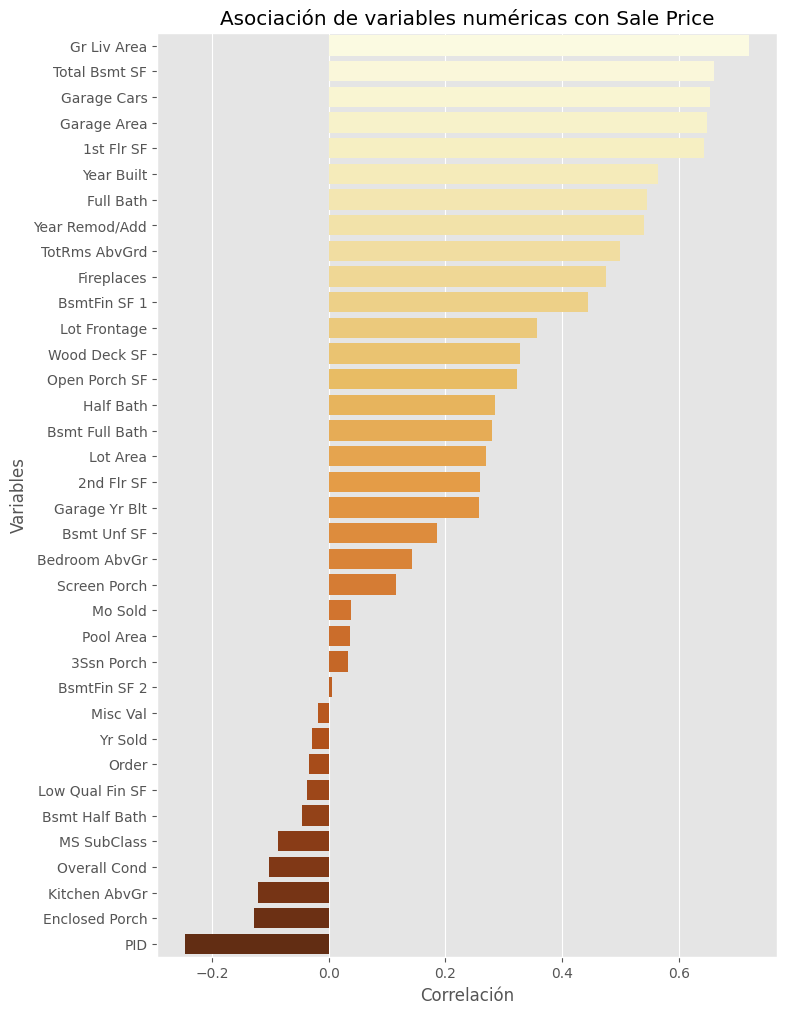
\includegraphics[width=0.5\textwidth]{figures/Asociacion de Variables Numericas con Sale Price.png}
	\caption[Asociación de variables numéricas con \textit{SalePrice}]{Asociación de variables numéricas con \textit{SalePrice}.}
	\label{fig:grafico numericas y SalePrice}
	\end{center}
\end{figure}

\begin{figure}[ht]
	\begin{center}
	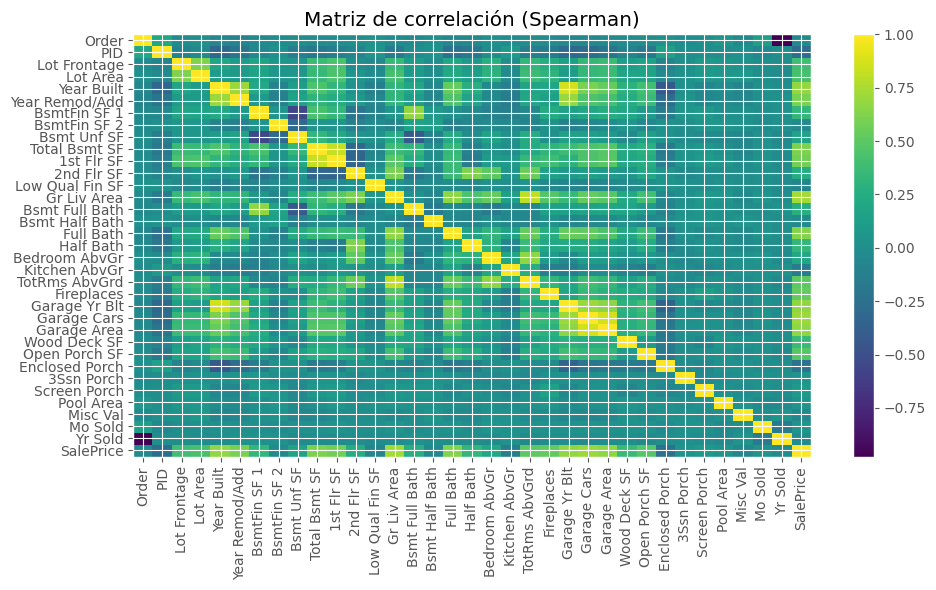
\includegraphics[width=0.5\textwidth]{figures/Matriz de Correlación Spearman.png}
	\caption[Matriz de correlación de \textit{Spearman} de variables cuantitativas]{Matriz de correlación de \textit{Spearman} de variables cuantitativas.}
	\label{fig:graficocuantitativospear}
	\end{center}
\end{figure}


\begin{figure}[ht]
	\begin{center}
	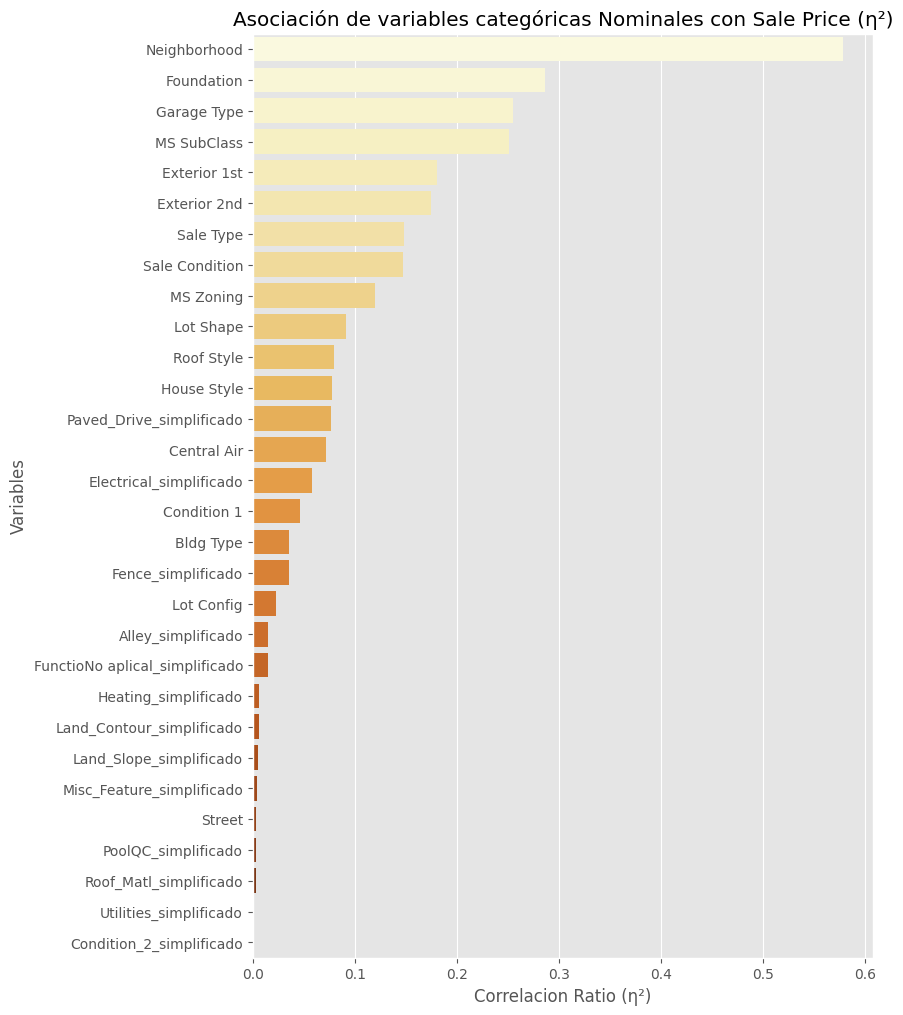
\includegraphics[width=0.5\textwidth]{figures/Asociación de variables categóricas nominales con Sale Price.png}
	\caption[Asociación de variables categóricas nominales con \textit{Sale Price}.]{Asociación de variables categóricas nominales con \textit{Sale Price}.}
	\label{fig:asociación categórica nominal con SP}
	\end{center}
\end{figure}

\begin{figure}[ht]
	\begin{center}
	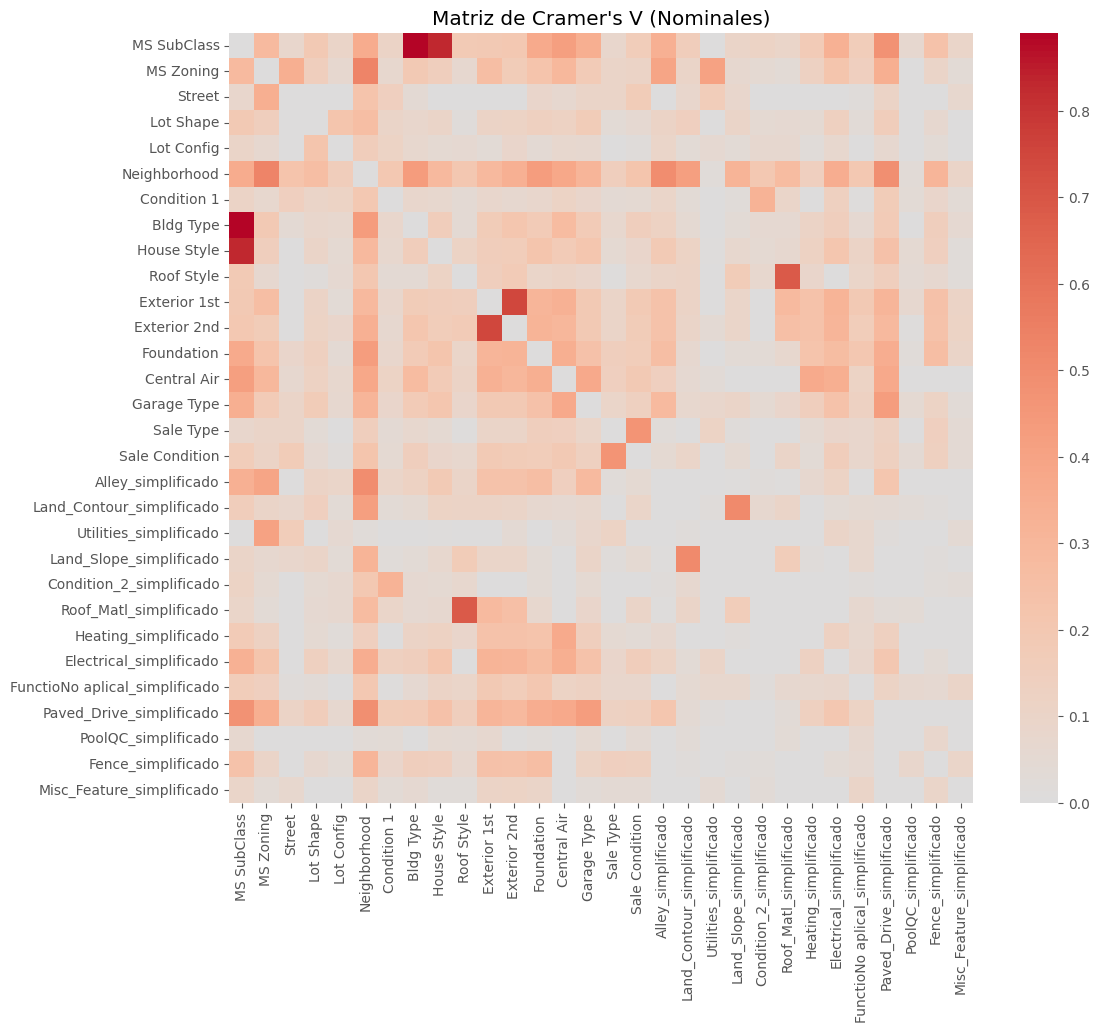
\includegraphics[width=0.5\textwidth]{figures/Matriz Cramer.png}
	\caption[Matriz de Cramer’s V de variables categóricas nominales]{Matriz de Cramer’s V de variables categóricas nominales.}
	\label{fig:cramerV nominales}
	\end{center}
\end{figure}
\clearpage
\begin{figure}[H]
	\begin{center}
	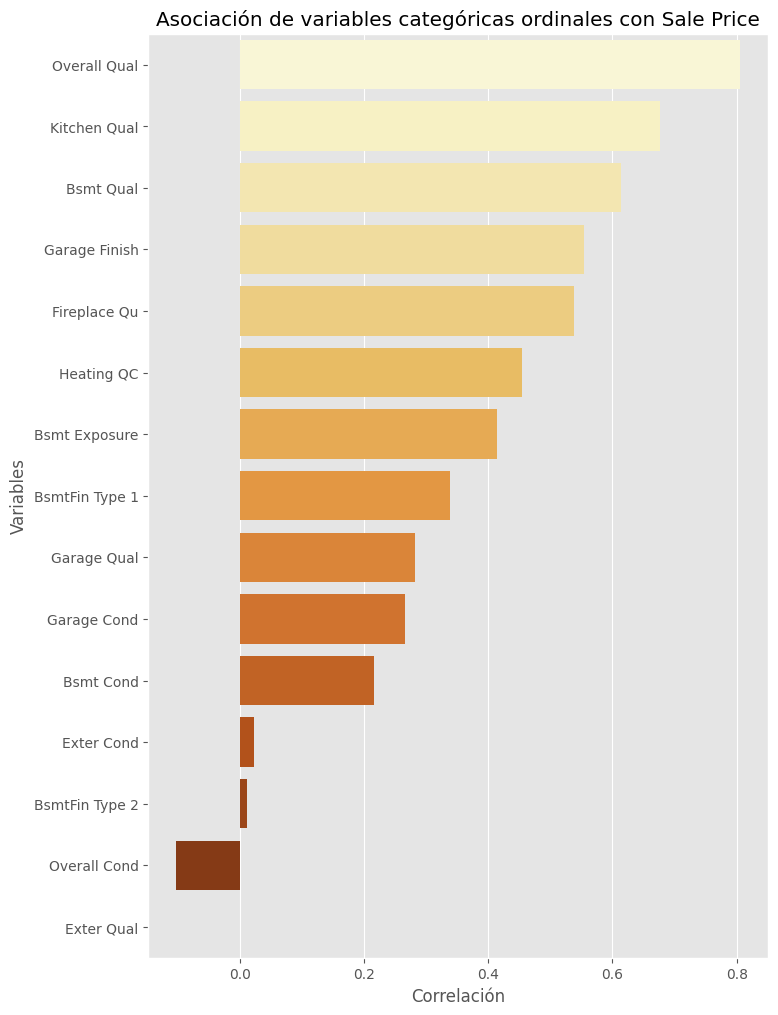
\includegraphics[width=0.5\textwidth]{figures/Asociación de variables categóricas ordinales con Sale Price.png}
	\caption[Asociación de variables categóricas Ordinales con \textit{Sale Price}.]{Asociación de variables categóricas Ordinales con \textit{Sale Price}.}
	\label{fig:precio con categorica ordinal}
	\end{center}
\end{figure}

\begin{figure}[ht]
	\begin{center}
	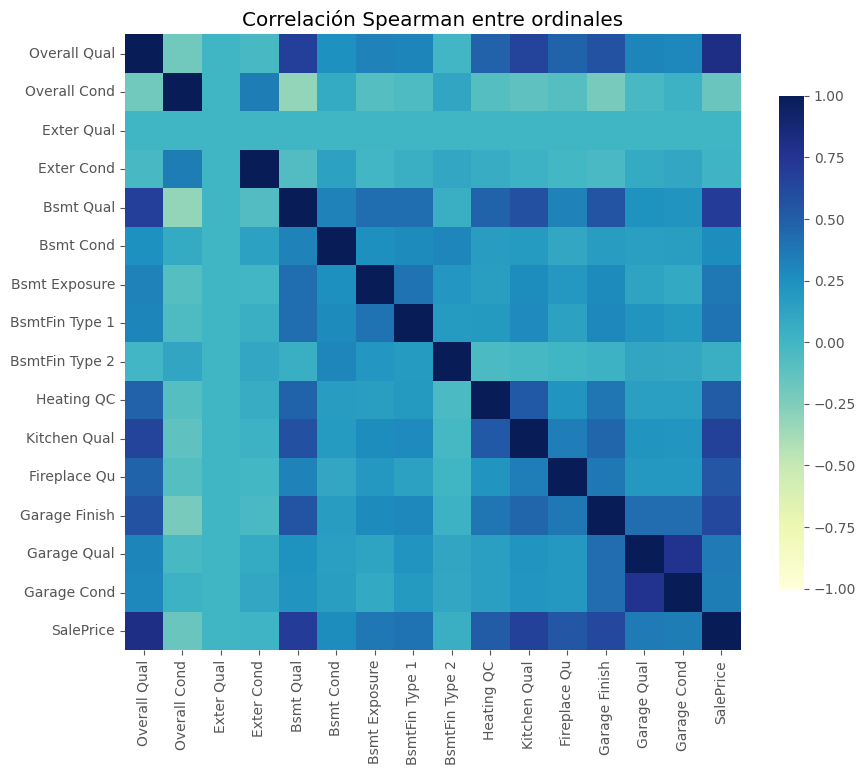
\includegraphics[width=0.5\textwidth]{figures/Correlación Spearman entre ordinales.png}
	\caption[Matriz de correlación de  Spearman de variables categóricas ordinales codificadas]{Matriz de correlación de Spearman de variables categóricas ordinales codificadas.}
	\label{fig:spearman categórica ordinal}
	\end{center}
\end{figure}

\begin{figure}[ht]
	\begin{center}
	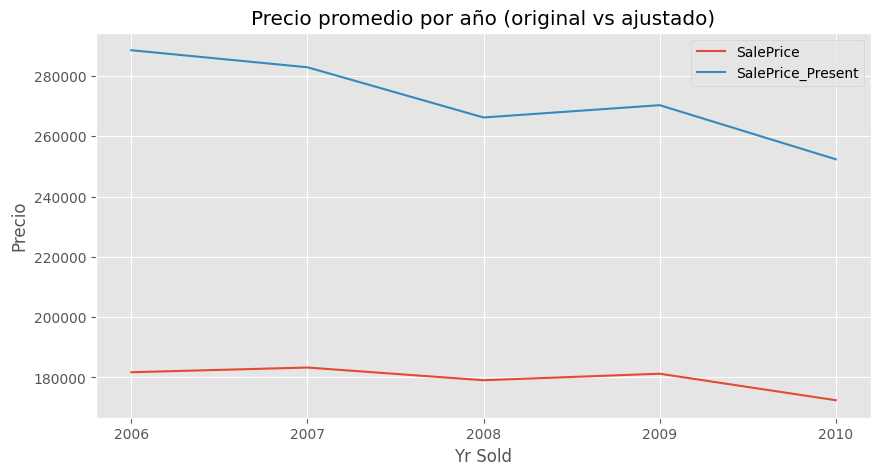
\includegraphics[width=0.5\textwidth]{figures/Ajuste IPC.png}
	\caption[Precio original vs ajustado]{Gráfico promedio de \textit{SalePrice} por año, ajustado por IPC al precio presente}
	\label{fig:Preciooriginalvsajustado}
	\end{center}
\end{figure}

\begin{figure}[ht]
	\begin{center}
	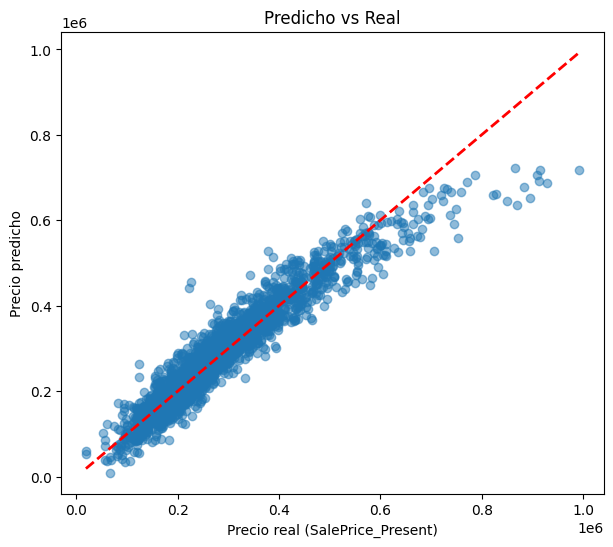
\includegraphics[width=0.5\textwidth]{figures/Regresion Normal.png}
	\caption[Regresión Lineal \textit{SalePrice\_Present}]{Regresión Lineal \textit{SalePrice\_Present}}
	\label{fig:regresioninicial}
	\end{center}
\end{figure}

\begin{figure}[ht]
	\begin{center}
	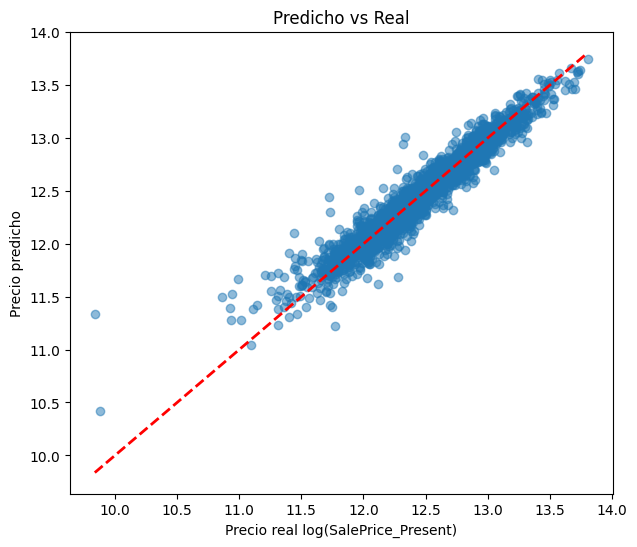
\includegraphics[width=0.5\textwidth]{figures/Regresion Log(Sale Price).png}
	\caption[Regresión Lineal \textit{log(SalePrice\_present)}.]{Regresión Lineal \textit{log(SalePrice\_present)}.}
	\label{fig:grafico logSalePrice con precio}
	\end{center}
\end{figure}

\begin{figure}[ht]
	\begin{center}
	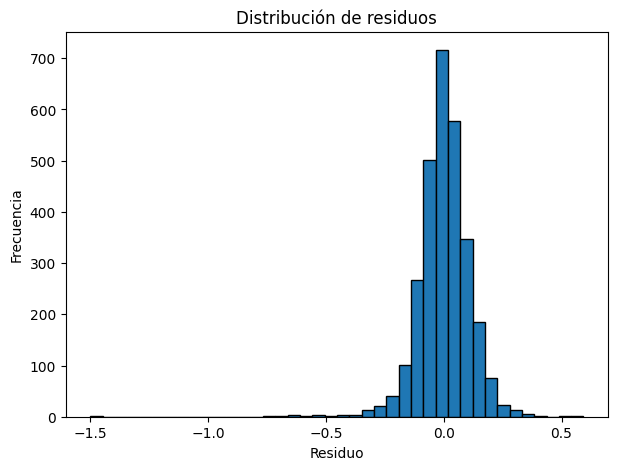
\includegraphics[width=0.5\textwidth]{figures/Residuos Regresión Log Sale Price .png}
	\caption[Distribución de residuos al aplicar \textit{log(SalePrice\_Present)}]{Distribución de residuos al aplicar \textit{log(SalePrice\_Present)}}
	\label{fig:distribucionderesiduoscon log}
	\end{center}
\end{figure}

\begin{figure}[ht]
    \centering
    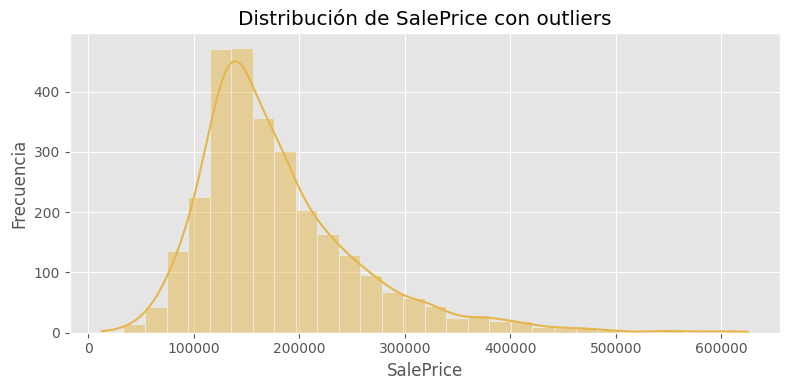
\includegraphics[width=0.5\textwidth]{figures/Distribución de Sale Price con Outliers.png}
    \caption[Distribución SalePrice]{Distribución de \textit{SalePrice} con \textit{outliers.}}
    \label{fig:residuos con outliers}
\end{figure}

\begin{figure}[ht]
	\begin{center}
	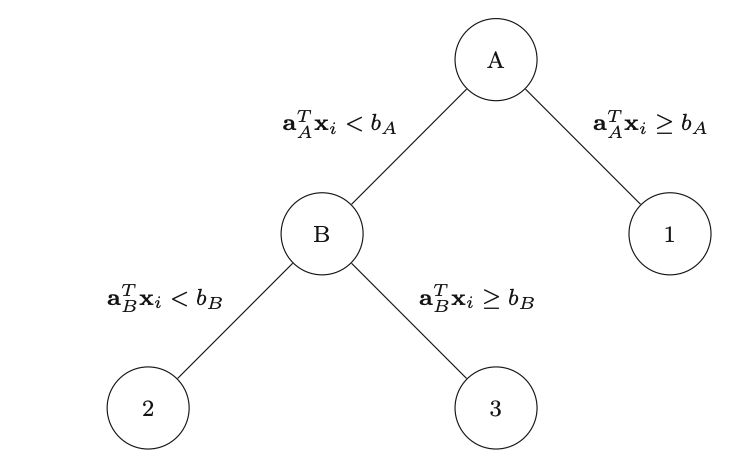
\includegraphics[width=0.5\textwidth]{figures/arboldecision.png}
	\caption[Árbol de decisión con dos nodos de partición y tres nodos hoja.]{Árbol de decisión con dos nodos de partición y tres nodos hoja. \cite{Bertsimas2017}}
	\label{fig:arboldecision}
	\end{center}
\end{figure}

\begin{figure}[ht]
\centering
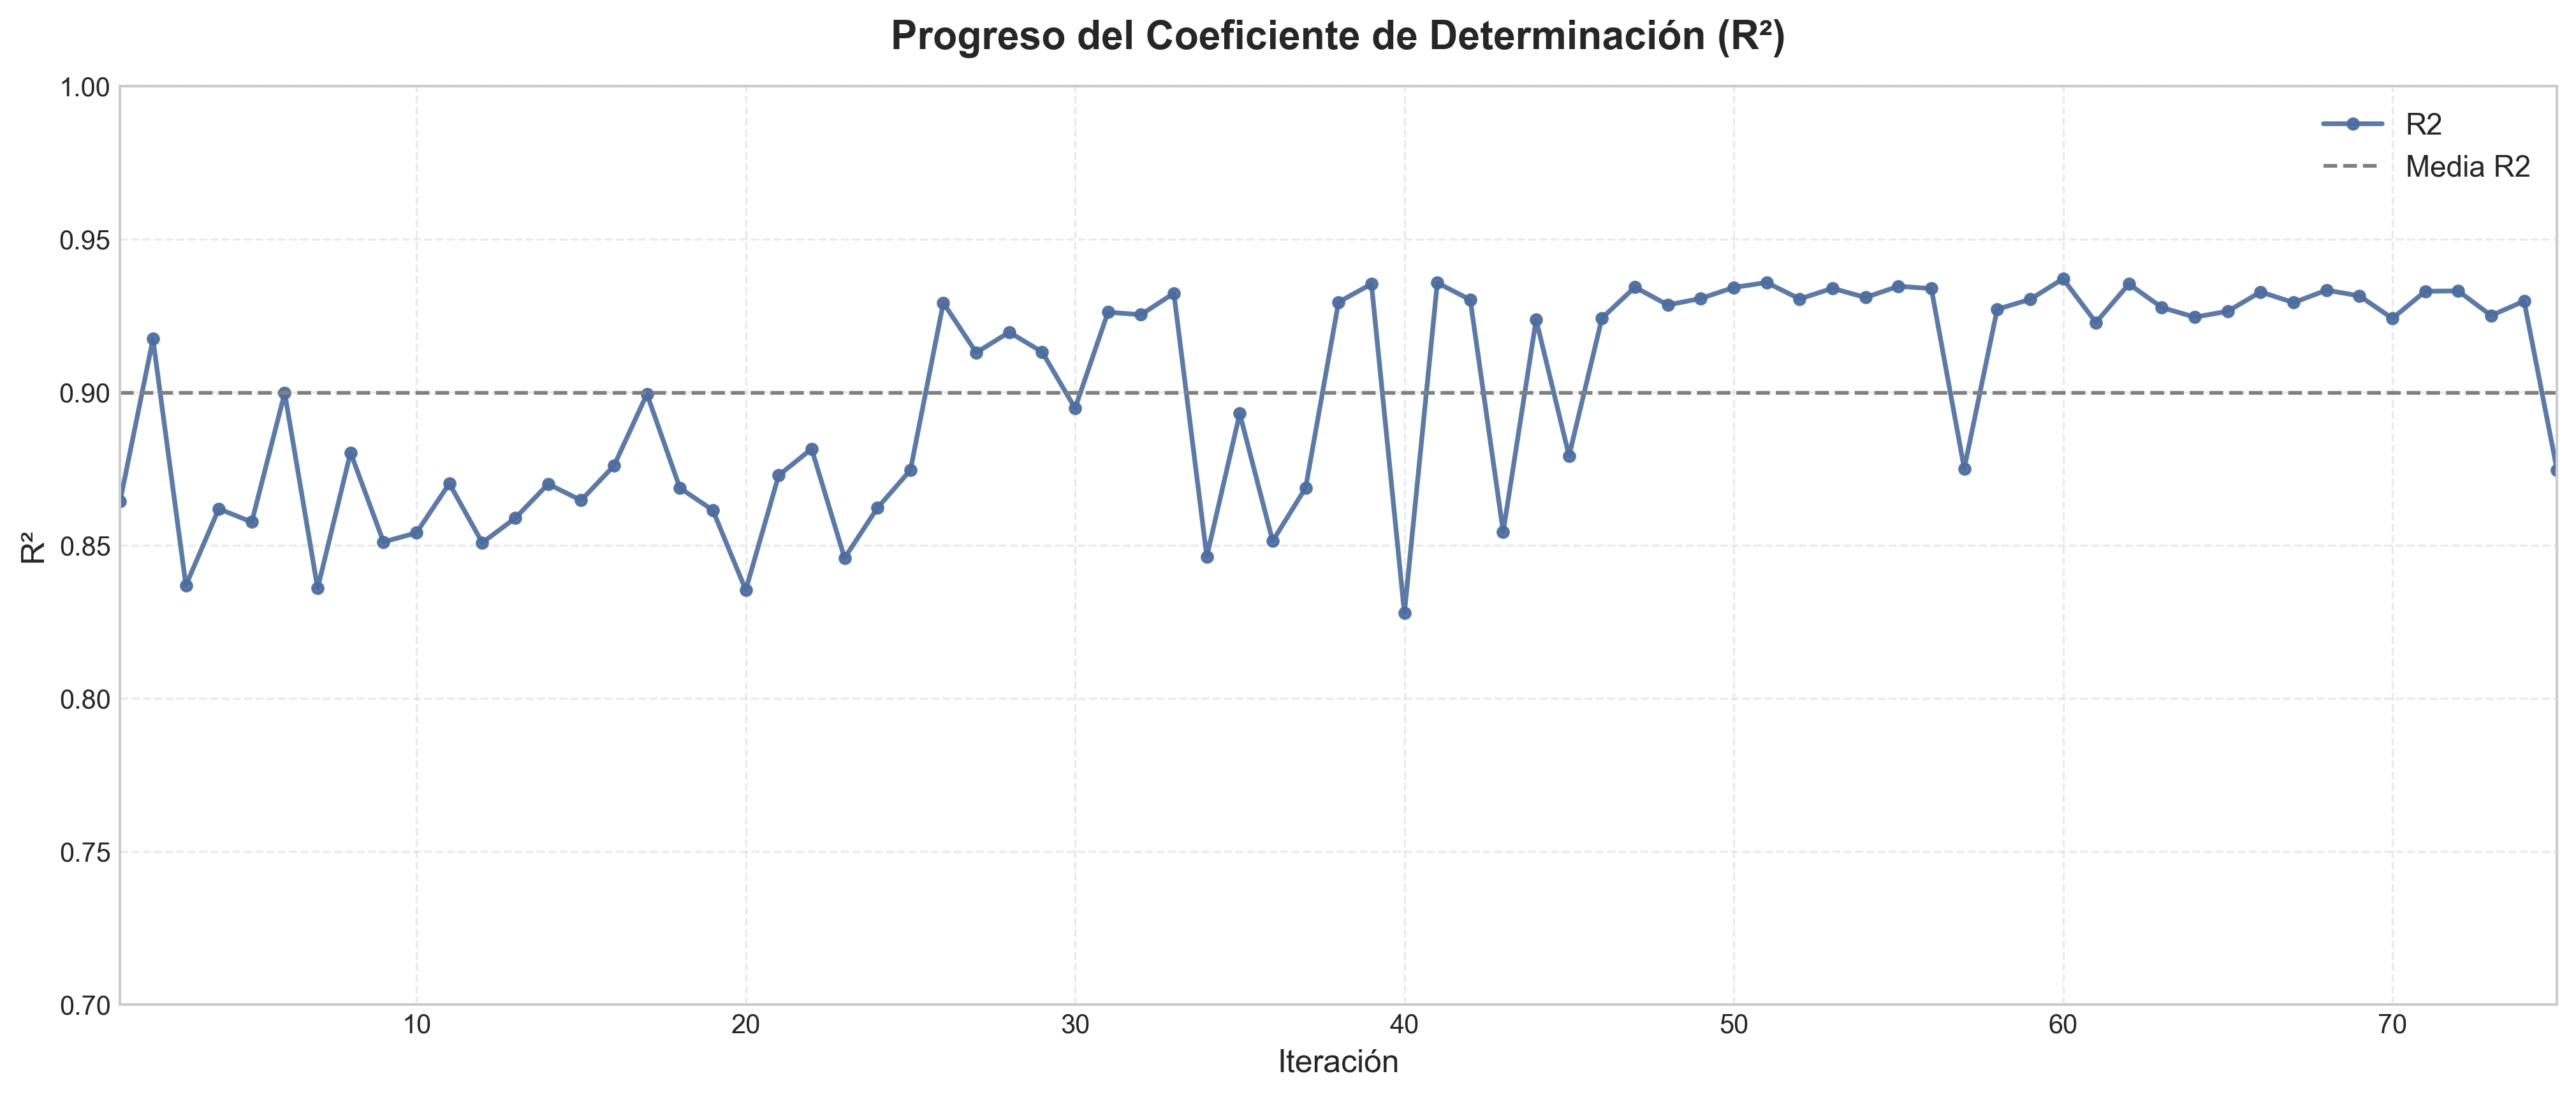
\includegraphics[width=0.6\textwidth]{figures/r2_iter_75.png}
\caption{Evoluci\'on $R^{2}$ con respecto al tiempo}
\label{fig:r2_iter}
\end{figure}

\begin{figure}[ht]
\centering
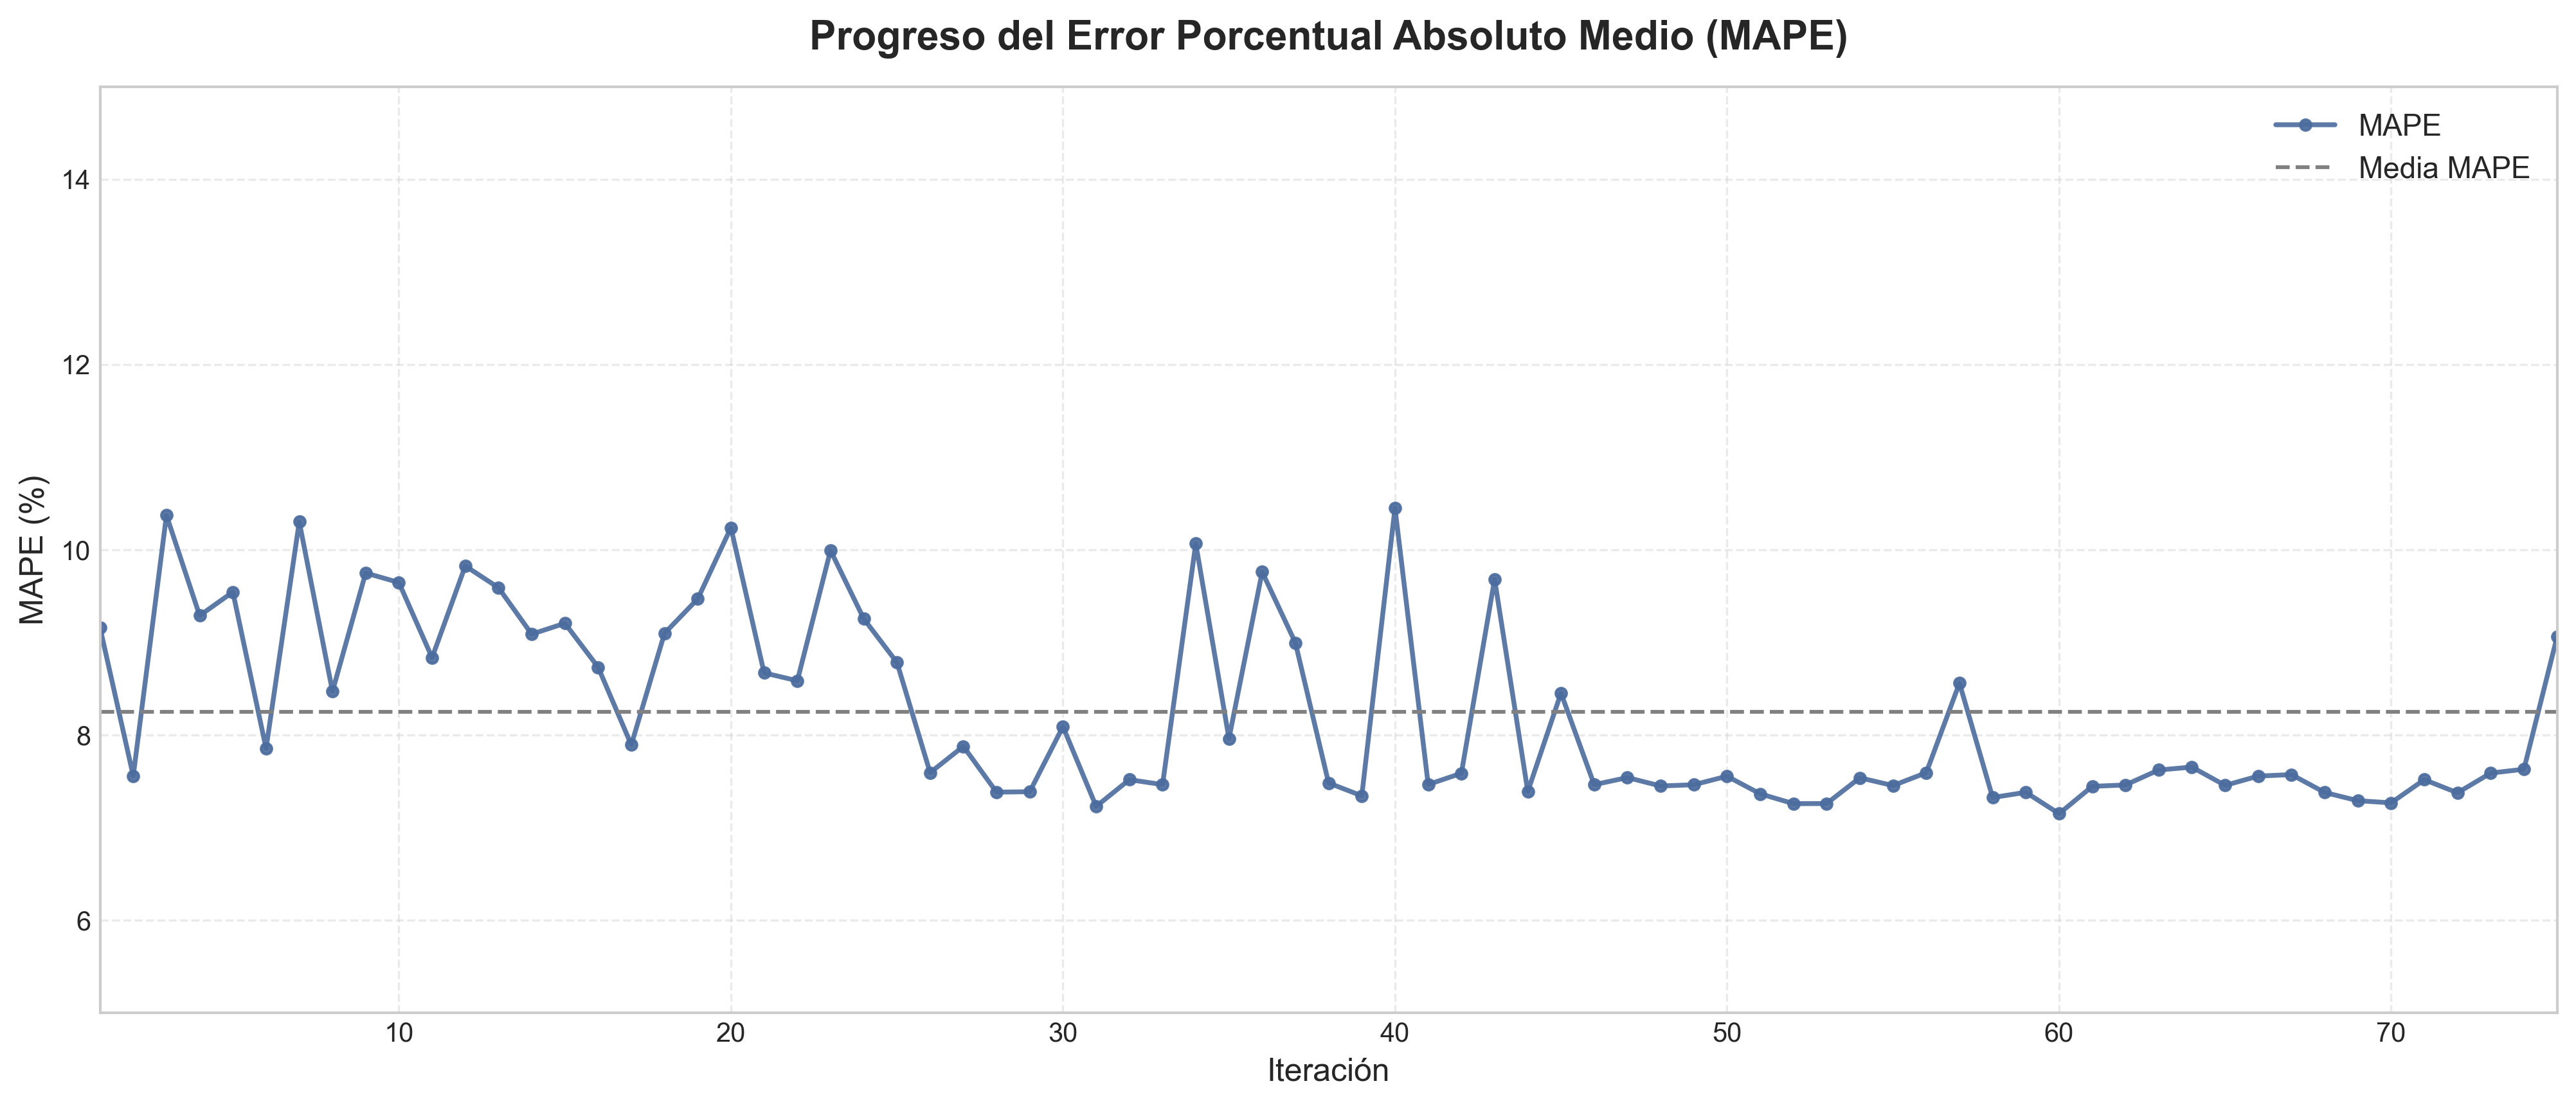
\includegraphics[width=0.6\textwidth]{figures/mape_iter_75.png}
\caption{Evoluci\'on MAPE con respecto al tiempo}
\label{fig:mape_iter}
\end{figure}

\begin{figure}[ht]
\centering
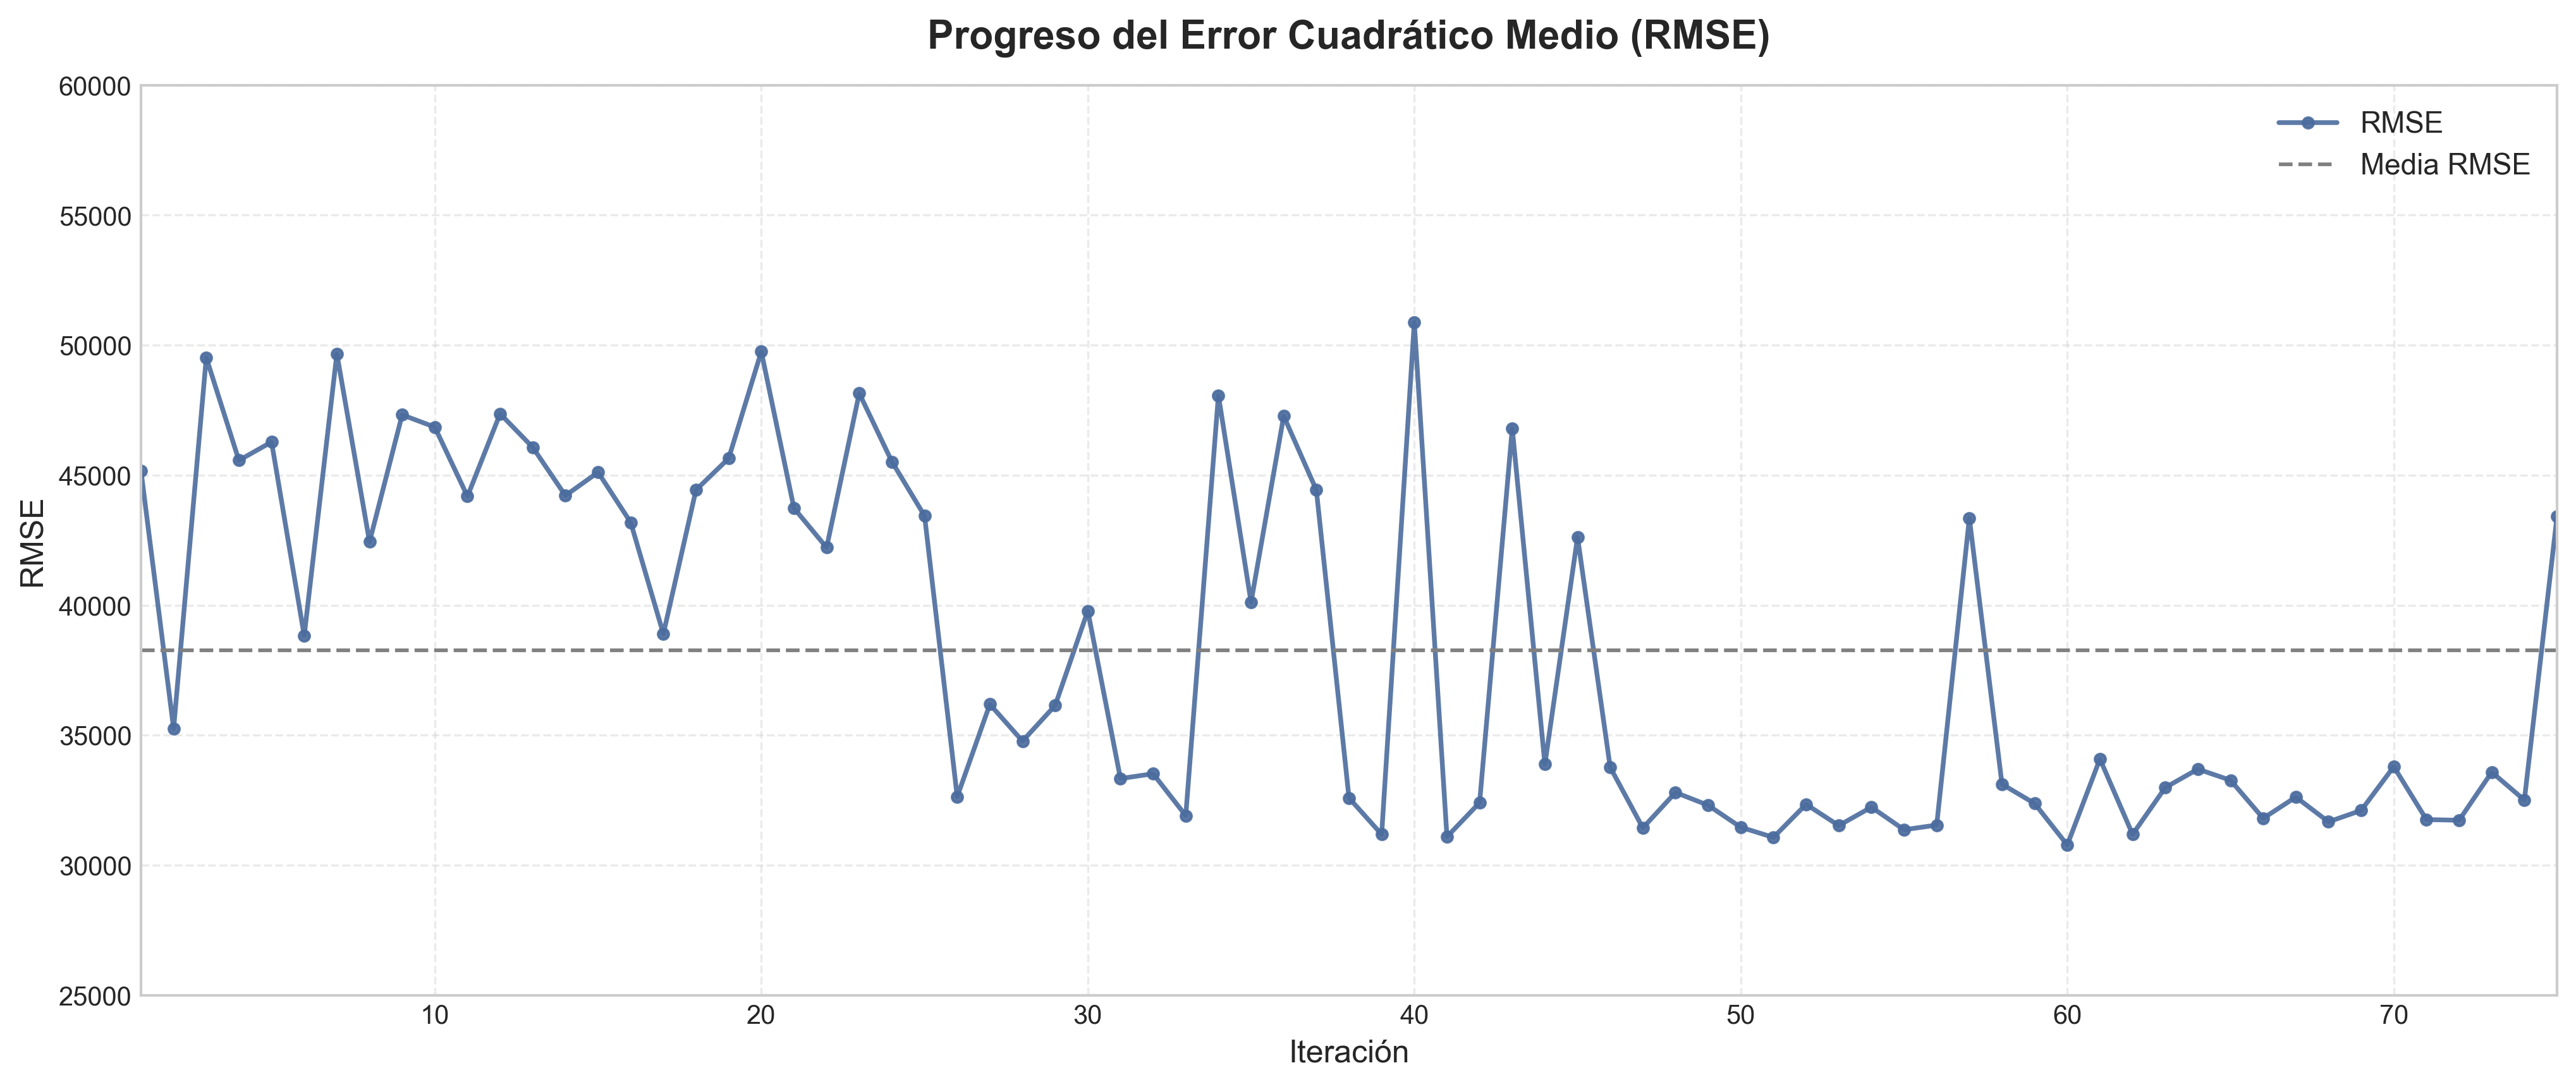
\includegraphics[width=0.6\textwidth]{figures/rmse_iter_75.png}
\caption{Evoluci\'on RMSE con respecto al tiempo}
\label{fig:rmse_iter}
\end{figure}

\begin{figure}[ht]
\centering
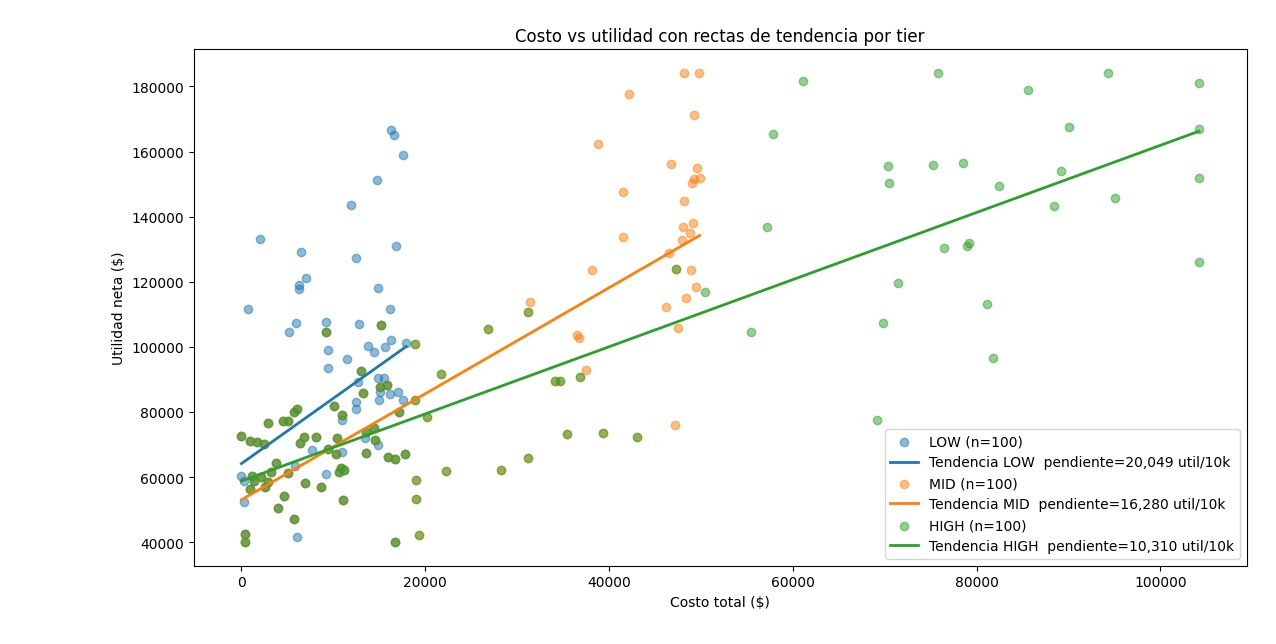
\includegraphics[width=0.6\textwidth]{figures/utilidad vs costo.jpg}
\caption{Diagrama Costo vs Utilidad con rectas de tendencia para los distintos presupuestos. Las pendientes representan la utilidad por cada 10k más de presupuesto.}
\label{fig:costo vs utilidad}
\end{figure}

\begin{figure}[ht]
	\begin{center}
	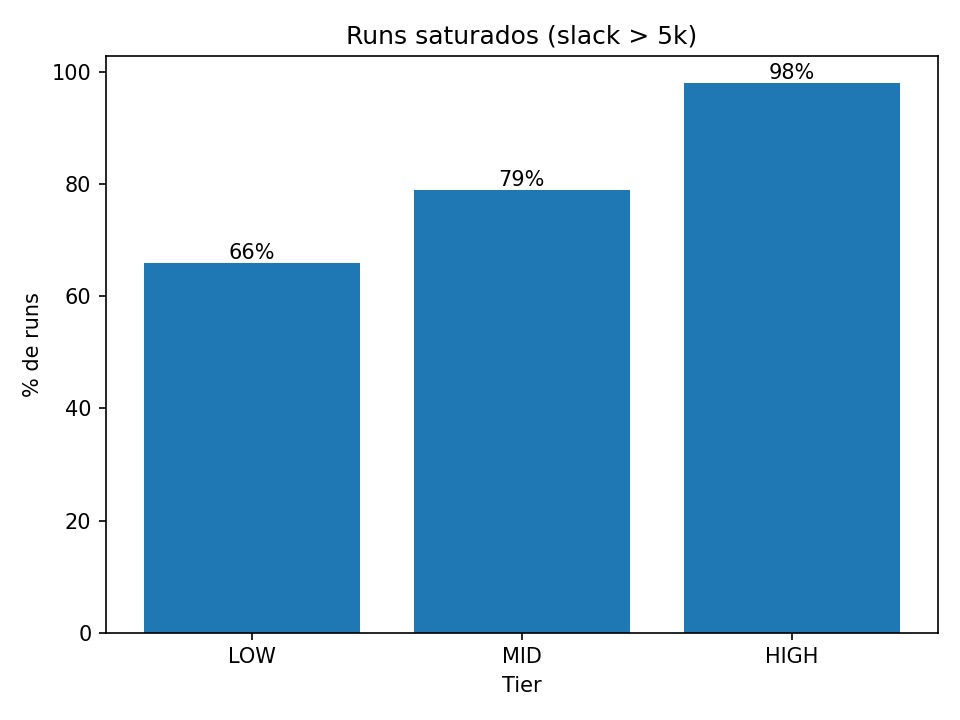
\includegraphics[width=0.5\textwidth]{figures/slacks saturados.jpg}
	\caption[]{Gráfico que muestra porcentaje de casas que les sobra más de 5K luego de la remodelación}
	\label{fig:slackssaturados}
	\end{center}
\end{figure}

\begin{figure}[ht]
	\begin{center}
	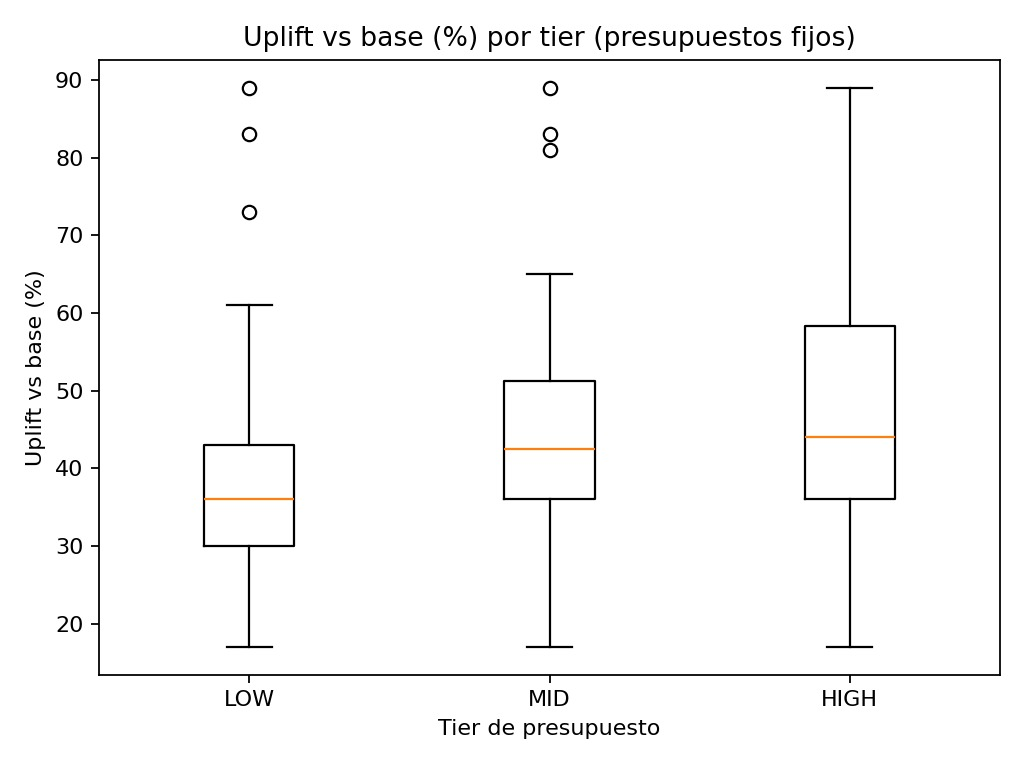
\includegraphics[width=0.5\textwidth]{figures/uplift vs base.jpg}
	\caption[]{Gráfico muestra que porcentaje de revalorizacion aumenta con presupuesto, pero con gran variabilidad}
	\label{fig:uplift}
	\end{center}
\end{figure}

\begin{figure}[ht]
	\begin{center}
	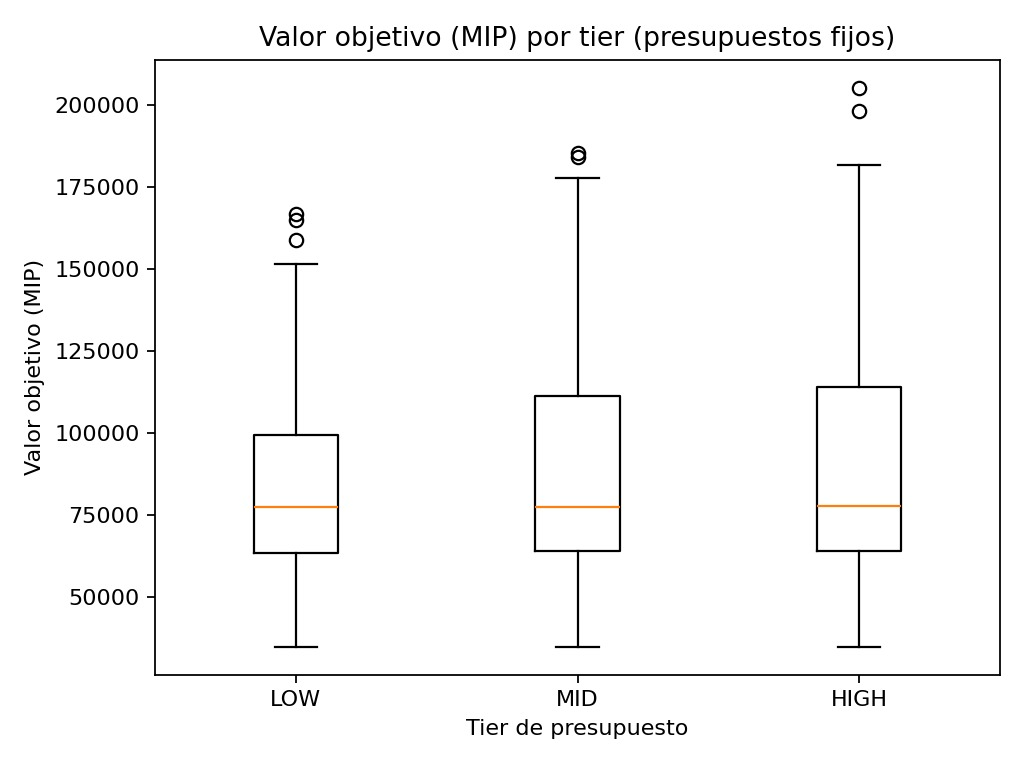
\includegraphics[width=0.5\textwidth]{figures/boxplotMIP.jpg}
	\caption[]{Gráfico muestra que medianas son parecidas entre tiers, pero la dispersion y los maximos crecen de low a mid a high.}
	\label{fig:boxplotMIP}
	\end{center}
\end{figure}

\begin{figure}[ht]
	\begin{center}
	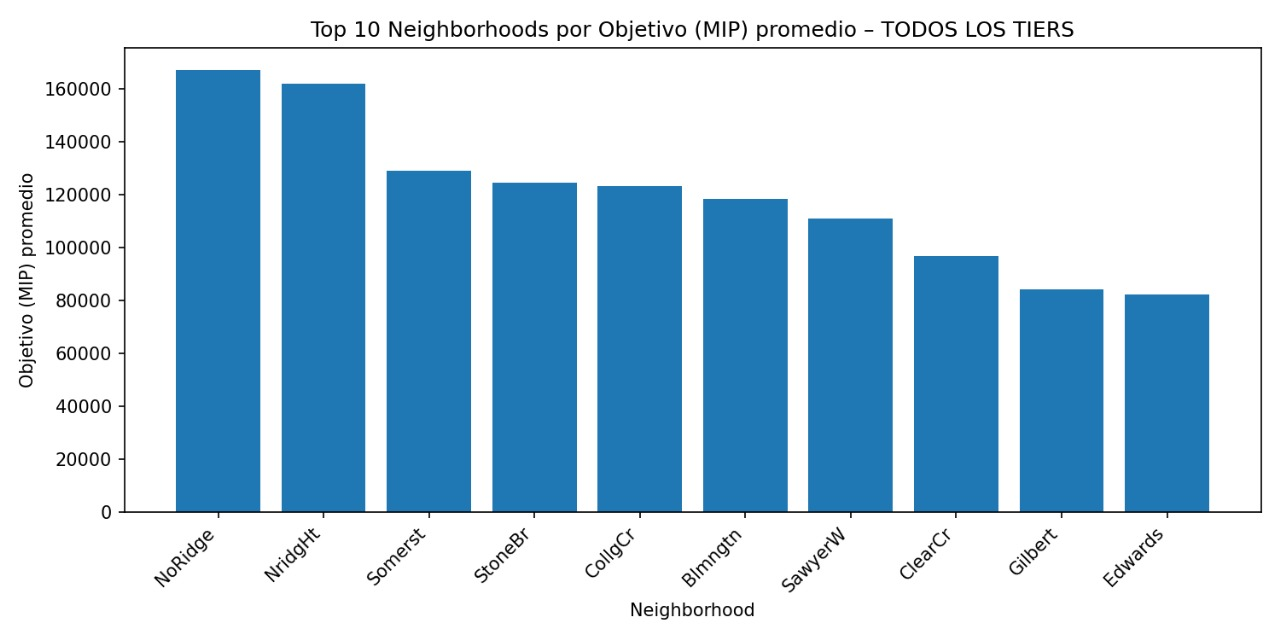
\includegraphics[width=0.5\textwidth]{figures/10 top neghborhoods.jpg}
	\caption[]{Gráfico muestra que medianas son parecidas entre tiers, pero la dispersion y los maximos crecen de low a mid a high.}
	\label{fig:top10NB}
	\end{center}
\end{figure}

\begin{figure}[ht]
	\begin{center}
	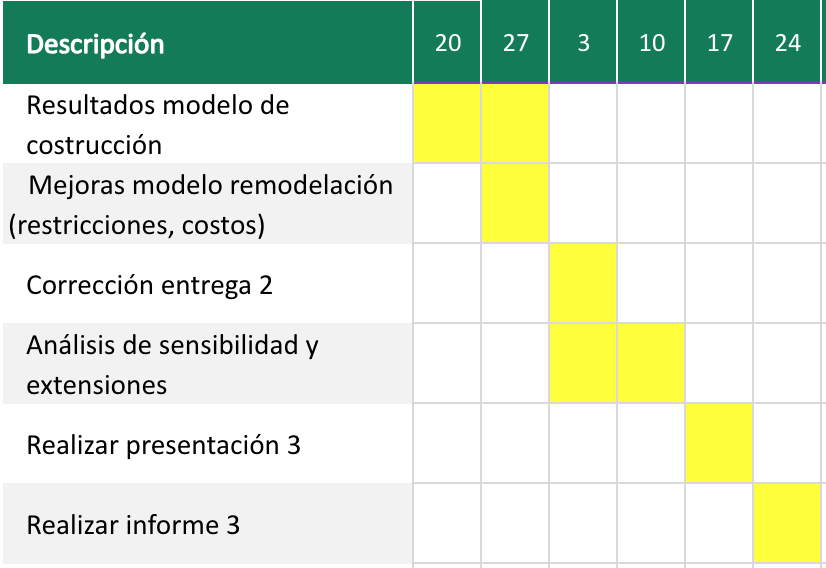
\includegraphics[width=0.5\textwidth]{figures/cartagantt.png}
	\caption[Carta Gantt]{Carta Gantt}
	\label{fig:CartaGantt}
	\end{center}
\end{figure}

\chapter{Árbol de decisión}\label{app:Árbol de decisión}
Para algunas de las restricciones más relevantes que se presentan a continuación nos basamos en lo que mencionan \cite{Bertsimas2017}.\\
- $x_{i} \in [0, 1]^{p}$\\
- $z_{it}$: binaria que indica si $x_{i}$ esta en el nodo t.\\
- $l_t$: binaria que indica si la hoja t contiene algún punto. \\
- $N_{\min}$: número mínimo de puntos en cada hoja.\\
- $c_{kt}$: binaria que indica si la clase asignada al nodo t es k.\\
- $p_{t}:$ predicción del nodo t.\\
- $A_{L}(t):$ conjunto de ancestros de t cuya rama izquierda se ha seguido en el camino desde el nodo raíz hasta t.\\
- $A_{R}(t):$ conjunto de ancestros de la rama derecha.\\
- $T_{H}:$ nodos hoja.\\
- $T_{R}:$ nodos rama.\\
- $M_{1}, M_{2}$: número ssuficientemente grandes.\\
- $\epsilon > 0$
\begin{itemize}
    \item Número mínimo de puntos en cada hoja.\[
z_{it} \le l_t, \qquad \forall t \in T_R
\]
    \[
\sum_{i=1}^{n} z_{it} \ge N_{\min} \, l_t, \qquad \forall t \in T_R
\]
    \item Cada punto se asigna a una hoja.
    \[
\sum_{t \in T_H} z_{it} = 1, \quad i = 1, \dots, n
\]
    \item Divisiones estructurales para la estructura del árbol al asignar puntos a las hojas.\[
a_{m}^{T} x_i \ge b_{m} - M_{2}(1 - z_{it}), \quad i = 1,\ldots,n,\ \forall t \in T_R,\ \forall m \in A_R(t)
\]
    No se puede quedar como inecuación por eso se agrega un $\epsilon$ que es un párametro pequeño para este otro caso.
    \[
a_{m}^{T} x_i + \varepsilon \le b_{m} + M_{1}(1 - z_{it}), 
\quad i = 1,\ldots,n,\ \forall t \in T_R,\ \forall m \in A_L(t)
\]
    \item Solo una predicción de clase en cada nodo hoja que contenga puntos. \[
\sum_{k=1}^{K} c_{kt} = l_t, \qquad \forall t \in T_H
\]
    \item Predicción para cada i.
    \[
    \sum_{t \in T_{H}}p_{t} z_{it}, \quad  i = 1, \ldots,n\
    \]
\end{itemize}


\chapter{Modelo Remodelación}\label{app:Remodelación}

%renovación
\section{Supuestos remodelación}
\label{sec:supuestos remodelación}
A continuación se detallan supuestos del modelo de remodelación.\\
1. La variable Foundation indica los cimientos de la casa, por lo que se fija como parámetro, ya que cambiarla implicaría destruir la casa completa.\\ 
2. La variable BsmtQual indica la altura del sótano y define su calidad según eso, no se procederá a cambiar esta calidad ya que implicaría cambiar la infraestructura de la casa. \\ 
3. No se considera expanción del sótano de la casa, ya que implicaría destrucción de cimientos de la casa y evaluaciones de suelo de los cuales no tenemos información. Por ende es por limitación de la base de datos.\\ 
4. No se agregaran chimeneas, ya que la variable Fireplaces contabiliza la cantidad total de chimeneas sin diferenciar cuales estan en la casa y cuáles en el sótano, por ende para restringir cúantas se puede agregar no se tendría un parámetro claro de máximo. Además, si se agregan no se sabría dónde por lo mismo. La desición esta tomada por la limitación de información de la base de datos.\\ 
5. Las variables Overall Qual y Overall Cond no se cambiaran, ya que indican la calidad y condiciones generales de la casa, por lo que depende de todos los otros factores de calidad y condición de la casa.\\  
6. La variable Functional que indica la evaluación cualitativa del estado funcional general de la vivienda no será modificada, esto debido a que no podemos hacer mejoras específicas si no tenemos conocimiento de qué es deficiente en particular. La desición esta tomada por la limitación de información de la base de datos.\\ 
7. La variable LowQualFinSF que indica pies cuadrados de mala calidad en todos los pisos no se cambiará. No podemos hacer mejoras específicas si no tenemos conocimiento de qué es deficiente en particular.La desición esta tomada por la limitación de información de la base de datos.\\
8. Para la renovación de espacios se considera que no se modificaran las habitaciones del interior de la casa, esto debido a que no existen especificaciones de los $f^{2}$ que hay de cada habitación, por ende esto limita su posible expansión y/o reducción. La desición esta tomada por la limitación de información de la base de datos.\\

\section{Costos remodelación}
\label{sec:costos remodelación}
${C^{Total}_{i}}$= 
\[
\;\;
\underbrace{\sum_{\substack{u \in \mathcal{U}^+_i \\ u \neq u_i^{\text{base}}}} \! C_u \; Utilities_{i,u}}_{\text{costo de nueva utility}}
\;+\;
\underbrace{
C^{\text{Roof}}_{\text{demolición}}
\;\sum_{\substack{m \in \mathcal{M}^+_i \\ m \neq m_i^{\text{base}}}}
y_{i,m}
}_{\text{demolición Roof}}
\;+\;
\underbrace{\sum_{\substack{m \in \mathcal{M}^+_i \\ m \neq m_i^{\text{base}}}} C_m\, y_{i,m}}_{\text{costo del nuevo material Roof}}
\]

\[
+\Bigg[
\underbrace{C^{(1)}_{(e_1)^{base}_i}\, (UpgMat_i - Change1_i)}_{\text{reconstruir material base 1}}\\[4pt]
\quad
+\underbrace{\sum_{\substack{e_1\in\mathcal{E}\\ e_1\neq (e_1)^{base}_i}}
C^{(1)}_{e_1}\, Exterior1st_{i,e_1}}_{\text{cambiar a material más caro 1}}\\[6pt]
\]
\[
+\underbrace{Has2_i\Big(\,
C^{(2)}_{(e_2)^{base}_i}\, (UpgMat_i - Change2_i)
+\,
\sum_{\substack{e_2\in\mathcal{E}\\ e_2\neq (e_2)^{base}_i}}
C^{(2)}_{e_2}\, Exterior2nd_{i,e_2}
\Big)}_{\text{Exterior 2 (si existe)}}\\[6pt]
\]

\[
+\underbrace{\sum_{\substack{eq\in\mathcal{Q}\\ BaseQual_{i,eq}=0}} C^{Q}_{eq}\, ExterQualSel_{i,eq}
+\sum_{\substack{ec\in\mathcal{C}\\ BaseCond_{i,ec}=0}} C^{C}_{ec}\, ExterCondSel_{i,ec}}_{\text{mejorar calidad/condición Exterior 1 y Exterior 2}}
\Bigg]
\]
\[
\;+\;
\underbrace{\sum_{\substack{t \in \mathcal{T}^+_i \\ t \neq t_i^{\text{base}}}}
\Big( C_t \cdot \mathrm{MasVnrArea}_i \Big)\; MasVnrType_{i,t}}_{\text{cambiar MasVnrArea o construirlo si no hay}}
\;+\;
\underbrace{\sum_{\substack{e \in \mathcal{E}^+_i \\ e \neq e_i^{\text{base}}}}
C_e\, Electrical_{i,e}}_{\text{costo del nuevo tipo Electrical}}
\]
\[
+\underbrace{\sum_{i \in \mathcal{I}:\ a_i^{\text{base}} = \text{No}} C_{\text{CentralAir}} \cdot CentralAir_{i,\text{Yes}}}_{\text{Costo de incluir CentralAir}}
\]
\[
+\underbrace{C_{\,h_i^{\text{base}}}\,(UpgType_i - ChangeType_i)}_{\text{reconstruir mismo tipo Heating}}\\[4pt]
+\underbrace{\sum_{h\in\mathcal{H}_i^+} C_h\, M^H_{i,h}\, Heating_{i,h}}_{\text{cambiar a tipo más caro de Heating}}\\[4pt]
+\underbrace{\sum_{q\in\mathcal{Q}_i^+} C_{hqc}\, M^{QC}_{i,q}\, HeatingQC_{i,q}}_{\text{cambiar calidad Heating}}
\]
\[
\;+\;
\underbrace{\sum_{\substack{k \in \mathcal{K}_{i,\text{allow}} \\ k \neq k_i^{\text{base}}}}
C_k \;\, KitchenQual_{i,k}}_{\text{cambiar calidad cocina}}
\;\;
+\underbrace{C_{\text{Bsmt}}
\Big( x^{(1)}_i + x^{(2)}_i \Big)}_{\text{terminar el sótano}}
\;+\;
\underbrace{\sum_{\substack{b \in \mathcal{B}_{i,\text{allow}} \\ b \neq b_i^{\text{base}}}}
C_b \;\, BsmtCond_{i,b}}_{\text{cambiar calidad sótano}}
\]

\[
+\underbrace{\sum_{b_1\in\mathcal{B}}
C_{BstmType}\, M^{B1}_{i,b}\, BsmtFinType1_{i,b}}_{\text{Costo por mejora en BsmtFinType1}}\\[4pt]
+\underbrace{HasB2_i
\sum_{b_2\in\mathcal{B}}
C_{BstmType}\, M^{B2}_{i,b}\, BsmtFinType2_{i,b}}_{\text{Costo por mejora en BsmtFinType2 (si existe)}}
\]

\[
\;+\;
\underbrace{\sum_{\substack{fen \in \mathcal{F}_{i,\text{allow}} \\ fen \neq f_i^{\text{base}}}}
C_{fen} \;\, FireplaceQu_{i,fen}}_{\text{Costo por mejorar Chimenea}}
  \;+\;
  \underbrace{\sum_{\substack{fen \in \mathcal{F}_{i,\text{allow}} \\ fen \neq f_i^{\text{base}}}}
  C_{Fence, fen}\;\, Fence_{i,fen}}_{\text{Costo por mejorar Fence}}
  \]

\[
  \;+\;
   \underbrace{\sum_{i \in \mathcal{I}: \ f_i^{\text{base}}=\text{NA}}
  C_{\text{Fence}} \cdot LotFrontage_i \cdot 
  \Big( Fence_{i,\text{MnPrv}} + Fence_{i,\text{GdPrv}} \Big)}_{\text{Costo por construir Fence}}
+\underbrace{\sum_{\substack{d \in \mathcal{D}_{i,\text{allow}} \\ d \neq d_i^{\text{base}}}}
C_d \; PavedDrive_{i,d}}_{\text{Costo por construir PavedDrive}}
\]

\[
\underbrace{+\sum_{g\in \mathcal{G}^{Q}_{i,\text{allow}}}
C_g\, M^{Q}_{i,g}\, GarageQual_{i,g}}_{\text{Costo por mejorar Calidad Garage}}
\;+\;
\underbrace{\sum_{g\in \mathcal{G}^{C}_{i,\text{allow}}}
C_g\, M^{C}_{i,g}\, GarageCond_{i,g}}_{\text{Costo por mejorar Condición Garage}}
\]


\[
\begin{aligned}
&+\,
\underbrace{
C_{\text{construccion}}
\Big(
A^{\text{Full}}\,AddFull_i
+ A^{\text{Half}}\,AddHalf_i
+ A^{\text{Kitch}}\,AddKitch_i
+ A^{\text{Bed}}\,AddBed_i
\Big)
}_{\text{(costo por construir habitación en particular)}}
\end{aligned}
\]


\[
 \;+\;\underbrace{ \sum_{c\in\mathcal{C}}
\Big( C^{10}_{c}\,\Delta^{10}_{i,c}\, z^{10}_{i,c} \;+\; C^{20}_{c}\,\Delta^{20}_{i,c}\, z^{20}_{i,c} \;+\; C^{30}_{c}\,\Delta^{30}_{i,c}\, z^{30}_{i,c} \Big)}_{\text{costo por ampliación}}
\;\;
+\underbrace{\sum_{\substack{p \in \mathcal{P}_{i,\text{allow}} \\ p \neq p_i^{\text{base}}}}
C_p \;\, PoolQC_{i,p}}_{\text{costo por mejorar la piscina}}
+\underbrace{\sum_{ga \in \mathcal{G}a}
C_{GFin} \;\, M^{Ga}_{i,ga} \;\, gar_{i,ga}}_{\text{costo por terminar el Garage}}
\]

\section{Restricciones remodelación}
\label{sec:restricciones remodelación}
A continuación se presenta el modelo realizado para el caso de remodelación. Con el fin de que se entienda mejor, las restricciones se van explicando por variable. Se utilizó como ayuda la IA Chat GPT para implementar las restricciones generalizadas a cada caso específico, el detalle se enseña en el siguiente link: https://chatgpt.com/share/68eb241e-1070-8005-a699-6e5cda4677d7

\begin{itemize}
    \item Utilities: Se puede cambiar a alternativas que sean de costo mayor o mantenerse. El costo de construcción de una nueva Utilitie considera la destrucción del anterior. \\
    - Parámetro de Utilitie original: 
\[
u_i^{\text{base}} \in u \qquad \forall i \in \mathcal{I}.
\]
 - Parámetro de Costo de la Utilitie original:
 \[
C_{u_i^{\text{base}}} \in u \qquad \forall i \in \mathcal{I}.
\]
 
-Definición de conjunto permitido de utilities 
\[
\mathcal{U}^+_i = \{\, u \in \{AllPub, NoSewr, NoSeWa, ELO\} : C_u \ge C_{u_i^{\text{base}}} \,\}.
\]

-Variables de decisión
\[
Utilities_{i,u} \in \{0,1\} \qquad \forall i \in \mathcal{I},\, \forall u \in \mathcal{U}^+_i.
\]

-Restricción
\[
\sum_{u \in \mathcal{U}^+_i} Utilities_{i,u} = 1 \qquad \forall i \in \mathcal{I}.
\]

-Si se realiza el cambio se incurre en un costo, en la FO agregar: 
\[
\text{CostoUtilities} \;=\;
\underbrace{\sum_{\substack{u \in \mathcal{U}^+_i \\ u \neq u_i^{\text{base}}}} \! C_u \; Utilities_{i,u}}_{\text{costo de la nueva utility}}
.
\]

    \item RoofStyle y RoofMatl:
Se selecciona un tipo de \textit{roof style} y un tipo de \textit{roof material} compatibles entre sí. El material y el estilo pueden mantenerse o cambiarse a una alternativa de costo mayor, respetando las compatibilidades constructivas.\\

    - Matriz de compatibilidad entre estilos y materiales:\\
    La compatibilidad se representa mediante el parámetro binario $A_{s,m}$, donde $A_{s,m} = 1$ si el material $m$ puede ser utilizado con el estilo $s$, y $A_{s,m} = 0$ en caso contrario.
    
    \[
    A_{s,m} =
    \begin{array}{c|cccccc}
     & \text{AsphaltShingle} & \text{Metal} & \text{ClayTile} & \text{WoodShingle} & \text{Slate} & \text{Membrane} \\
    \hline
    \text{Gable}   & 1 & 1 & 1 & 1 & 1 & 0 \\
    \text{Hip}     & 1 & 1 & 1 & 1 & 1 & 0 \\
    \text{Flat}    & 0 & 1 & 0 & 0 & 0 & 1 \\
    \text{Mansard} & 1 & 1 & 1 & 1 & 1 & 0 \\
    \text{Shed}    & 1 & 1 & 0 & 1 & 0 & 1 \\
    \end{array}
    \]
    Esta matriz fue construida en base a compatibilidades constructivas reportadas en fuentes técnicas de cubiertas 
    \cite{roofcrafters2024, renoworks2023, wikipediaFlatRoof2024}.\\

    - Parámetro de Roof Style original:
    \[
    s_i^{\text{base}} \in s \qquad \forall i \in \mathcal{I}.
    \]

    - Parámetro de Roof Material original:
    \[
    m_i^{\text{base}} \in m \qquad \forall i \in \mathcal{I}.
    \]

    - Parámetro de costo de Roof Style y Roof Material:
    \[
    \, C_m \qquad \, \forall m \in m.
    \]

    - Definición de conjuntos permitidos:
    \[
    \mathcal{S}^+_i = \{\, s \in \{Flat, Gable, Gambrel, Hip, Mansard, Shed\} : C_s \ge C_{s_i^{\text{base}}} \,\}\]
   \[
    \mathcal{M}^+_i = \{\,m\in\{ClyTile, CompShg, Membran, Metal, Roll, TarGrv, WdShake, WdShngl\:C_m \ge C_{m_i^{\text{base}}} \,\}.
    \]
    - Variables de decisión:
    \[
    x_{i,s} \in \{0,1\} \qquad \forall i \in \mathcal{I},\, \forall s \in \mathcal{S}^+_i,
    \]
    \[
    y_{i,m} \in \{0,1\} \qquad \forall i \in \mathcal{I},\, \forall m \in \mathcal{M}^+_i.
    \]
    - Restricción de selección única:
    \[
    \sum_{s \in \mathcal{S}^+_i} x_{i,s} = 1 \qquad \forall i \in \mathcal{I}, \qquad
    \sum_{m \in \mathcal{M}^+_i} y_{i,m} = 1 \qquad \forall i \in \mathcal{I}.
    \]

    - Restricción de compatibilidad entre estilo y material según la matriz $A_{s,m}$.:
    \[
    x_{i,s} + y_{i,m} \le 1 
    \qquad \forall i \in \mathcal{I},\, \forall s \in \mathcal{S}^+_i,\, \forall m \in \mathcal{M}^+_i : A_{s,m} = 0.
    \]
    
    - Parámetro de costo de demolición grande:
\[
C^{\text{Roof}}_{\text{demolición}} \ge 0.
\]

- Si se realiza el cambio de material se incurre en costo, en la FO agregar:

\[
\text{CostoRoof}
\;=\;
\underbrace{
C^{\text{Roof}}_{\text{demolición}}
\;\sum_{\substack{m \in \mathcal{M}^+_i \\ m \neq m_i^{\text{base}}}}
y_{i,m}
}_{\text{demolición Roof}}
\;+\;
\underbrace{\sum_{\substack{m \in \mathcal{M}^+_i \\ m \neq m_i^{\text{base}}}} C_m\, y_{i,m}}_{\text{costo del nuevo material}}
\]


    \item Exterior1st, Exterior2nd, ExterQual, ExterCond: Si la calidad o condición del material exterior presenta un indice de Average/Typical o inferior, entonces se pueden seguir dos caminos. El primero es que el material del Exterior1st y el Exterior2nd pueden mantenerse recostruyendo cada uno denuevo o reemplazarse por otro de costo superior al actual. Exterior2nd solo aplica si existe un segundo material en la casa. El segundo es que ExterQual y ExterCond puedan cambiar aumentando su calidad y condición respectivamente.\\

   - Materiales:
\[
\begin{aligned}
\mathcal{E} = \{&
\text{AsbShng},\ \text{AsphShn},\ \text{BrkComm},\ \text{BrkFace},\
\text{CBlock},\ \text{CemntBd},\ \text{HdBoard},\ \text{ImStucc},\\
&\text{MetalSd},\ \text{Other},\ \text{Plywood},\ \text{PreCast},\
\text{Stone},\ \text{Stucco},\ \text{VinylSd},\ \text{WdSdng},\ \text{WdShing}\}.
\end{aligned}
\]


- Parámetros de costos de materiales:
\[
C^{(1)}_e \ \forall e\in\mathcal{E}, \qquad
C^{(2)}_e \ \forall e\in\mathcal{E}.
\]
- Parámetros de costos de calidad/condición:
\[
\mathcal{Q}=\{\text{Ex},\text{Gd},\text{TA},\text{Fa},\text{Po}\},\quad
\mathcal{C}=\{\text{Ex},\text{Gd},\text{TA},\text{Fa},\text{Po}\},
\]
\[
C^{Q}_{eq}\ \forall eq\in\mathcal{Q}, \qquad C^{C}_{ec}\ \forall ec\in\mathcal{C}.
\]
- Costos de demolición por frente (aplican sólo si se toma el camino material):
\[
C^{dem}_{1}\ge 0,\qquad C^{dem}_{2}\ge 0.
\]

- Parámetros base:
\[
(e_1)^{base}_i \in \mathcal{E}, \qquad
(e_2)^{base}_i \in \mathcal{E}\ \ \text{si } Has2_i=1,
\]
\[
BaseQual_{i,eq}\in\{0,1\},\ \sum_{eq\in\mathcal{Q}} BaseQual_{i,eq}=1,\qquad
BaseCond_{i,ec}\in\{0,1\},\ \sum_{ec\in\mathcal{C}} BaseCond_{i,ec}=1,
\]
\[
Has2_i\in\{0,1\}.
\]
- Subconjuntos “Average o peor”:
\[
\mathcal{Q}^{\le Av}=\{\text{TA},\text{Fa},\text{Po}\},\qquad
\mathcal{C}^{\le Av}=\{\text{TA},\text{Fa},\text{Po}\}.
\]
- Parámetros costos base:
\[
C^{Q,\text{base}}_i=\sum_{eq} C^Q_{eq}\, BaseQual_{i,eq},\qquad
C^{C,\text{base}}_i=\sum_{ec} C^C_{ec}\, BaseCond_{i,ec}.
\]

- Selección final de materiales:
\[
Exterior1st_{i,e_1}\in\{0,1\}\ \forall e_1\in\mathcal{E},\ \ 
\sum_{e_1} Exterior1st_{i,e_1}=1,
\]
\[
Exterior2nd_{i,e_2}\in\{0,1\}\ \forall e_2\in\mathcal{E},\ \
\sum_{e_2} Exterior2nd_{i,e_2}=Has2_i.
\]
- Variables finales de calidad y condición:
\[
ExterQualSel_{i,eq}\in\{0,1\},\ \sum_{eq} ExterQualSel_{i,eq}=1,
\]
\[
ExterCondSel_{i,ec}\in\{0,1\},\ \sum_{ec} ExterCondSel_{i,ec}=1.
\]

- Binarias de caminos y elegibilidad:
\[
UpgMat_i,\, UpgQC_i,\, Eligible_i \in\{0,1\}.
\]
- Detección de cambio de material:
\[
Change1_i,\, Change2_i \in \{0,1\}.
\]

-Activación binarias:
\[
Eligible_i \ \ge\ \sum_{eq\in\mathcal{Q}^{\le Av}} BaseQual_{i,eq},\qquad
Eligible_i \ \ge\ \sum_{ec\in\mathcal{C}^{\le Av}} BaseCond_{i,ec},
\]
\[
Eligible_i \ \le\ \sum_{eq\in\mathcal{Q}^{\le Av}} BaseQual_{i,eq}
           + \sum_{ec\in\mathcal{C}^{\le Av}} BaseCond_{i,ec}.
\]
-Restricción de caminos excluyentes:
\[
UpgMat_i + UpgQC_i \ \le\ Eligible_i.
\]

-Restricción de que no empeora calidad ni condición:
\[
Exterior1st_{i,e_1}=0\ \ \forall e_1:\ C^{(1)}_{e_1} < C^{(1)}_{(e_1)^{base}_i},
\]
\[
Exterior2nd_{i,e_2}=0\ \ \forall e_2:\ C^{(2)}_{e_2} < C^{(2)}_{(e_2)^{base}_i},
\]
\[
ExterQualSel_{i,eq}=0\ \ \forall eq:\ C^Q_{eq} < C^{Q,\text{base}}_i,\qquad
ExterCondSel_{i,ec}=0\ \ \forall ec:\ C^C_{ec} < C^{C,\text{base}}_i.
\]

-Restricciones material sólo cambia si se toma el camino material:
\[
\sum_{\substack{e_1\in\mathcal{E}\\ e_1\neq (e_1)^{base}_i}} Exterior1st_{i,e_1} \ \le\ UpgMat_i,
\]
\[
\sum_{\substack{e_2\in\mathcal{E}\\ e_2\neq (e_2)^{base}_i}} Exterior2nd_{i,e_2} \ \le\ UpgMat_i \cdot Has2_i.
\]

\[
\sum_{\substack{eq\in\mathcal{Q}\\ BaseQual_{i,eq}=0}} ExterQualSel_{i,eq} \ \le\ UpgQC_i,
\]
\[
\sum_{\substack{ec\in\mathcal{C}\\ BaseCond_{i,ec}=0}} ExterCondSel_{i,ec} \ \le\ UpgQC_i.
\]

-Restricciones de exclusion:
\[
\sum_{\substack{eq\in\mathcal{Q}\\ BaseQual_{i,eq}=0}} ExterQualSel_{i,eq} \ \le\ 1 - UpgMat_i,
\]
\[
\sum_{\substack{ec\in\mathcal{C}\\ BaseCond_{i,ec}=0}} ExterCondSel_{i,ec} \ \le\ 1 - UpgMat_i,
\]
\[
\sum_{\substack{e_1\in\mathcal{E}\\ e_1\neq (e_1)^{base}_i}} Exterior1st_{i,e_1} \ \le\ 1 - UpgQC_i,
\]
\[
\sum_{\substack{e_2\in\mathcal{E}\\ e_2\neq (e_2)^{base}_i}} Exterior2nd_{i,e_2} \ \le\ (1 - UpgQC_i)\cdot Has2_i.
\]
-Restricciones de cambio de material:
\[
Change1_i \ \ge\ Exterior1st_{i,e_1} \quad \forall e_1\neq (e_1)^{base}_i,\qquad
Change1_i \ \le\ \sum_{\substack{e_1\in\mathcal{E}\\ e_1\neq (e_1)^{base}_i}} Exterior1st_{i,e_1},
\]
\[
Change2_i \ \ge\ Exterior2nd_{i,e_2} \quad \forall e_2\neq (e_2)^{base}_i,\qquad
Change2_i \ \le\ \sum_{\substack{e_2\in\mathcal{E}\\ e_2\neq (e_2)^{base}_i}} Exterior2nd_{i,e_2}.
\]

-Si se realiza el cambio se incurre en un costo, donde la construcción del nuevo material incluye el costo de demolición, en la FO agregar:\\

\text{CostoMaterialExterior=}
\[
\begin{aligned}
& \Bigg[
\underbrace{C^{(1)}_{(e_1)^{base}_i}\, (UpgMat_i - Change1_i)}_{\text{reconstruir material base 1}}\\[4pt]
&\quad
+\underbrace{\sum_{\substack{e_1\in\mathcal{E}\\ e_1\neq (e_1)^{base}_i}}
C^{(1)}_{e_1}\, Exterior1st_{i,e_1}}_{\text{cambiar a material más caro 1}}\\[6pt]
&\quad
+\underbrace{Has2_i\Big(
C^{(2)}_{(e_2)^{base}_i}\, (UpgMat_i - Change2_i)
+\,
\sum_{\substack{e_2\in\mathcal{E}\\ e_2\neq (e_2)^{base}_i}}
C^{(2)}_{e_2}\, Exterior2nd_{i,e_2}
\Big)}_{\text{frente 2 sólo si existe}}\\[6pt]
&\quad
+\underbrace{\sum_{\substack{eq\in\mathcal{Q}\\ BaseQual_{i,eq}=0}} C^{Q}_{eq}\, ExterQualSel_{i,eq}
+\sum_{\substack{ec\in\mathcal{C}\\ BaseCond_{i,ec}=0}} C^{C}_{ec}\, ExterCondSel_{i,ec}}_{\text{mejorar calidad/condición}}
\Bigg].
\end{aligned}
\]

    \item MasVnrType: Se puede cambiar a alternativas de mayor costo o mantenerse. Si la tipología base es \text{None}, también se permite \emph{construir} una tipología distinta a \text{None} pagando su costo por pie cuadrado multiplicado por el área de revestimiento.


- Parámetro de tipo original:
\[
  t_i^{\text{base}} \in t \qquad \forall i \in \mathcal{I}.
\]

- Costo por tipo (por ft$^2$):
\[
  C_t \qquad \forall t \in \{BrkCmn, BrkFace, CBlock, None, Stone\}.
\]

- Área de revestimiento a considerar (ft$^2$):
\[
  \mathrm{MasVnrArea}_i \ge 0 \qquad \forall i \in \mathcal{I}.
\]

- Conjunto permitido (quedarse o subir):
\[
  \mathcal{T}^+_i \;=\; \left\{\, t \in \{BrkCmn, BrkFace, CBlock, None, Stone\} \ :\ C_t \ge C_{\,t_i^{\text{base}}} \,\right\}.
\]

- Variables de decisión:
\[
  MasVnrType_{i,t} \in \{0,1\} \qquad \forall i \in \mathcal{I},\ \forall t \in \mathcal{T}^+_i.
\]

- Selección única:
\[
  \sum_{t \in \mathcal{T}^+_i} MasVnrType_{i,t} \;=\; 1
  \qquad \forall i \in \mathcal{I}.
\]

- Si se realiza el cambio (o se construye desde \text{None}) se incurre en un costo proporcional al área. En la FO agregar:

\[
\text{CostoMasVnr}
\;=\;
\sum_{\substack{t \in \mathcal{T}^+_i \\ t \neq t_i^{\text{base}}}}
\Big( C_t \cdot \mathrm{MasVnrArea}_i \Big)\; MasVnrType_{i,t}.
\]

 \item Electrical: Se puede cambiar a alternativas que sean de costo mayor o mantenerse.\\
    -Conjunto:
    \[
      \mathcal{E} \;=\; \{SBrkr, FuseA, FuseF, FuseP, Mix\}.
    \]
    - Parámetro de tipo eléctrico original:
    \[
      e_i^{\text{base}} \in  \mathcal{E}\qquad \forall i \in \mathcal{I}.
    \]
    
    - Parámetro de costo por tipo eléctrico:
    \[
      C_e \qquad \forall e \in \mathcal{E}.
    \]

    - Definición de conjunto permitido:
    \[
      \mathcal{E}^+_i \;=\; \{\, e \in \mathcal{E} : C_e \ge C_{\,e_i^{\text{base}}} \,\}.
    \]

    - Variables de decisión:
    \[
      Electrical_{i,e} \in \{0,1\} \qquad \forall i \in \mathcal{I},\, \forall e \in \mathcal{E}^+_i.
    \]

    - Restricción:
    \[
      \sum_{e \in \mathcal{E}^+_i} Electrical_{i,e} \;=\; 1
      \qquad \forall i \in \mathcal{I}.
    \]
  
     - Si se realiza el cambio se incurre en un costo, donde el costo de construcción incluye el costo de demolición, en la FO agregar:
    \[
\text{CostoElectrical}
=
\underbrace{\sum_{\substack{e \in \mathcal{E}^+_i \\ e \neq e_i^{\text{base}}}}
C_e\, Electrical_{i,e}}_{\text{costo del nuevo tipo eléctrico}}
\]

\item CentralAir: Si la casa no tiene aire central, se permite mantener No o cambiar a Yes, incurriendo en el costo de implementación. Si la casa ya tiene aire central, se mantiene en Yes.

    - Parámetro de estado original de Central Air:
    \[
      a_i^{\text{base}} \in a \qquad \forall i \in \mathcal{I}.
    \]

    - Costo de implementación de Central Air:
    \[
      C_{\text{CentralAir}}
    \]
    - Conjunto permitido por ítem:
    \[
      \mathcal{A}_{i,\text{allow}} =
      \begin{cases}
        \{\text{Yes}\} & \text{si } a_i^{\text{base}} = \text{Yes},\\[3pt]
        \{\text{No},\, \text{Yes}\} & \text{si } a_i^{\text{base}} = \text{No}.
      \end{cases}
    \]
    - Variables binarias:
    \[
      CentralAir_{i,a} \in \{0,1\}
      \qquad \forall i \in \mathcal{I},\ \forall a \in \mathcal{A}_{i,\text{allow}}.
    \]
    - Selección única:
    \[
      \sum_{a \in \mathcal{A}_{i,\text{allow}}} CentralAir_{i,a} \;=\; 1
      \qquad \forall i \in \mathcal{I}.
    \]

    - Si se realiza el cambio se incurre en un costo, en la FO agregar:
    \[
    \text{CostoCentralAir}
=
      \sum_{i \in \mathcal{I}:\ a_i^{\text{base}} = \text{No}} C_{\text{CentralAir}} \cdot CentralAir_{i,\text{Yes}}.
    \]
    
    \item Heating y Heating QC: Si HeatingQC es \emph{Average/Typical} o peor, entonces pueden decidirse dos camino. EL primero es que el tipo de \textit{Heating} puede mantenerse construyéndolo denuevo o cambiarse a uno de mayor costo que el actual. El segundo, es que HeatingQC puede cambiar aumentando su calidad a una mejor.

- Tipos de Heating:
\[
  \mathcal{H}=\{\text{Floor},\text{GasA},\text{GasW},\text{Grav},\text{OthW},\text{Wall}\}.
\]
- Calidades de HeatingQC:
\[
  \mathcal{Q}=\{\text{Ex},\ \text{Gd},\ \text{TA},\ \text{Fa},\ \text{Po}\},\qquad
  \mathcal{Q}^{\le Av}=\{\text{TA},\ \text{Fa},\ \text{Po}\}.
\]

- Parámetros de costos:
\[
  C_h \ \ \forall h\in\mathcal{H}, \qquad C_{hqc} \ \ \forall hqc\in\mathcal{Q},\qquad
  C_{\text{destrucción}} \ge 0.
\]

- Parámetros de tipo base y calidad base:
\[
  h_i^{\text{base}}\in\mathcal{H},\qquad
  BaseQC_{i,q}\in\{0,1\},\ \sum_{q\in\mathcal{Q}} BaseQC_{i,q}=1.
\]

- Conjuntos “no empeorar” respecto a la base:
\[
  \mathcal{H}_i^+=\{\,h\in\mathcal{H}\ :\ C_h \ge C_{\,h_i^{\text{base}}}\,\},
  \qquad
  \mathcal{Q}_i^+=\{\,q\in\mathcal{Q}\ :\ C_{q} \ge \sum_{q'\in\mathcal{Q}} C_{q'}\, BaseQC_{i,q'}\,\}.
\]

- Parámetros máscara (para identificar opciones distintas del tipo o calidad base):
\[
M^H_{i,h} = 
\begin{cases}
1, & \text{si } h \neq h_i^{\text{base}},\\
0, & \text{si } h = h_i^{\text{base}},
\end{cases}
\qquad
M^{QC}_{i,q} = 1 - BaseQC_{i,q}.
\]

- Variables de decisión:
\[
  Heating_{i,h}\in\{0,1\}\ \ \forall h\in\mathcal{H}_i^+,\qquad
  \sum_{h\in\mathcal{H}_i^+} Heating_{i,h}=1,
\]
\[
  HeatingQC_{i,q}\in\{0,1\}\ \ \forall q\in\mathcal{Q}_i^+,\qquad
  \sum_{q\in\mathcal{Q}_i^+} HeatingQC_{i,q}=1.
\]

- Binarias de \textit{caminos} (excluyentes) y elegibilidad:
\[
  UpgType_i,\ UpgQC_i,\ Eligible_i \in \{0,1\}\qquad \forall i.
\]
- Binaria auxiliar para detectar cambio de tipo:
\[
  ChangeType_i \in \{0,1\} \qquad \forall i.
\]

- Activación binaria:
\[
  Eligible_i \ \ge\ \sum_{q\in\mathcal{Q}^{\le Av}} BaseQC_{i,q},\qquad
  Eligible_i \ \le\ \sum_{q\in\mathcal{Q}^{\le Av}} BaseQC_{i,q}.
\]
\[
  UpgType_i + UpgQC_i \ \le\ Eligible_i.
\]

- Cambio de tipo o calidad sólo si se toma el camino correspondiente:
\[
  \sum_{h\in\mathcal{H}_i^+} M^H_{i,h}\, Heating_{i,h} \ \le\ UpgType_i,
\]
\[
  \sum_{q\in\mathcal{Q}_i^+} M^{QC}_{i,q}\, HeatingQC_{i,q} \ \le\ UpgQC_i.
\]

- Exclusión de caminos simultáneos:
\[
  \sum_{q\in\mathcal{Q}_i^+} M^{QC}_{i,q}\, HeatingQC_{i,q} \ \le\ 1 - UpgType_i,
\]
\[
  \sum_{h\in\mathcal{H}_i^+} M^H_{i,h}\, Heating_{i,h} \ \le\ 1 - UpgQC_i.
\]

- Definición exacta de cambio de tipo:
\[
ChangeType_i \;=\; \sum_{h\in\mathcal{H}_i^+} M^H_{i,h}\, Heating_{i,h}.
\]

- Si se realiza el cambio se incurre en un costo, donde el costo de construcción incluye el costo de demolición, en la FO agregar:

\[
\begin{aligned}
&\text{CostoHeating}
=\underbrace{C_{\,h_i^{\text{base}}}\,(UpgType_i - ChangeType_i)}_{\text{reconstruir mismo tipo}}\\[4pt]
&\quad
+\underbrace{\sum_{h\in\mathcal{H}_i^+} C_h\, M^H_{i,h}\, Heating_{i,h}}_{\text{cambiar a tipo más caro}}\\[4pt]
&\quad
+\underbrace{\sum_{q\in\mathcal{Q}_i^+} C_{hqc}\, M^{QC}_{i,q}\, HeatingQC_{i,q}}_{\text{cambiar calidad}}
\end{aligned}
\]

    \item KitchenQual: La calidad de la cocina puede aumentar si es Typical/Average o peor.

    - Conjunto de calidades posibles:
    \[
      \mathcal{K} = \{\text{Ex},\ \text{Gd},\ \text{TA},\ \text{Fa},\ \text{Po}\}.
    \]

    - Parámetro de costo:
    \[
      C_k \qquad \forall k \in \mathcal{K}.
    \]

    - Parámetro de categoría base por ítem:
    \[
      k_i^{\text{base}} \in \mathcal{K} \qquad \forall i \in \mathcal{I}.
    \]
    - Subconjunto “Average/Typical o peor”:
    \[
      \mathcal{K}^{\le Av} = \{\text{TA},\ \text{Fa},\ \text{Po}\}.
    \]

    - Variables binarias de estado de calidad:
    \[
      KitchenQual_{i,k} \in \{0,1\} \quad \forall i \in \mathcal{I},\ \forall k \in \mathcal{K}.
    \]
    \[
      \sum_{k \in \mathcal{K}} KitchenQual_{i,k} = 1 \qquad \forall i \in \mathcal{I}.
    \]

    - Variable de activación de mejora:
    \[
      UpgKitch_i \in \{0,1\} \qquad \forall i \in \mathcal{I}.
    \]

    - Restricciones de activación:
    \[
      UpgKitch_i \;\ge\; KitchenQual_{i,k} \qquad \forall i \in \mathcal{I},\ \forall k \in \mathcal{K}^{\le Av},
    \]
    \[
      UpgKitch_i \;\le\; \sum_{k \in \mathcal{K}^{\le Av}} KitchenQual_{i,k} \qquad \forall i \in \mathcal{I}.
    \]
    - Conjunto permitido dependiente de $UpgKitch_i$:
    \[
      \mathcal{K}_{i,\text{allow}} =
      \begin{cases}
        \{\, k_i^{\text{base}} \,\} & \text{si } UpgKitch_i = 0,\\[4pt]
        \{\, k \in \mathcal{K} : C_k \ge C_{\,k_i^{\text{base}}} \,\} & \text{si } UpgKitch_i = 1.
      \end{cases}
    \]

    - Variables binarias prefiltradas:
    \[
      KitchenQual_{i,k} \in \{0,1\} \qquad \forall i \in \mathcal{I},\ \forall k \in \mathcal{K}_{i,\text{allow}}.
    \]
    - Selección única dentro del conjunto permitido:
    \[
      \sum_{k \in \mathcal{K}_{i,\text{allow}}} KitchenQual_{i,k} = 1 \qquad \forall i \in \mathcal{I}.
    \]

    - Si se realiza el cambio se incurre en un costo, en la FO agregar:
    \[
      \text{CostoKitchen}
      \;=\;
      \sum_{\substack{k \in \mathcal{K}_{i,\text{allow}} \\ k \neq k_i^{\text{base}}}}
      C_k \;\, KitchenQual_{i,k}.
    \]

    \item BsmtFinSF1, BsmtFinSF2, BsmtUnfSF, TotalBsmtSF: Si existe área no terminada del sótano (BsmtUnfSF $> 0$), se da la posibilida de terminarla, reasignando toda esa superficie a las zonas terminadas 1 y/o 2. Si se decide terminar, se termina completamente.

  - Parámetros base por ítem:
  \[
    (BsmtFinSF1)_i^{base} \in \mathbb{Z}_{\ge 0},
\]
 \[
    (BsmtFinSF2)_i^{base} \in \mathbb{Z}_{\ge 0},
\]
  \[
    (BsmtUnfSF)_i^{base} \in \mathbb{Z}_{\ge 0},\quad
    \]
      \[
    (TotalBsmtSF)_i^{base} \in \mathbb{Z}_{\ge 0},
  \]
  con
  \[
    (TotalBsmtSF)_i^{base}
    \;=\;
    (BsmtFinSF1)_i^{base}
    + (BsmtFinSF2)_i^{base}
    + (BsmtUnfSF)_i^{base}
    \qquad \forall i \in \mathcal{I}.
  \]

  - Variables de desición:
  \[
    BsmtFinSF1_{i} \in \mathbb{Z}_{\ge 0},
    BsmtFinSF2_{i} \in \mathbb{Z}_{\ge 0},\quad
    BsmtUnfSF_{i} \in \mathbb{Z}_{\ge 0}
    \qquad \forall i \in \mathcal{I}.
  \]

  - Variable binaria de decisión para “terminar completamente el sótano”:
  \[
    FinishBSMT_i \in \{0,1\} \qquad \forall i \in \mathcal{I}.
  \]

  - Variables de transferencia de superficie:
  \[
    x^{(1)}_{i},\, x^{(2)}_{i} \in \mathbb{Z}_{\ge 0} \qquad \forall i \in \mathcal{I}.
  \]

  - Conservación del total de sótano:
  \[
    BsmtFinSF1_i + BsmtFinSF2_i + BsmtUnfSF_i = (TotalBsmtSF)_i^{base}
    \qquad \forall i \in \mathcal{I}.
  \]

  - Todo o nada sobre el área sin terminar:
  \[
    BsmtUnfSF_i = (1 - FinishBSMT_i)\,(BsmtUnfSF)_i^{base}
    \qquad \forall i \in \mathcal{I}.
  \]

  - Definición de las zonas terminadas mediante la transferencia:
  \[
    BsmtFinSF1_i = (BsmtFinSF1)_i^{base} + x^{(1)}_i,\qquad
    BsmtFinSF2_i = (BsmtFinSF2)_i^{base} + x^{(2)}_i
    \qquad \forall i \in \mathcal{I}.
  \]

  - Si se termina, se transfiere \textbf{toda} el área no terminada:
  \[
    x^{(1)}_i + x^{(2)}_i = (BsmtUnfSF)_i^{base}\, FinishBSMT_i
    \qquad \forall i \in \mathcal{I}.
  \]
  - Si se termina de construir el sótano se incurre en un costo por pie cuadrado construido ($C_{Bsmt}$), en la FO agregar:
  \[
    \text{CostoTerminarBsmt}
    \;=\;
    C_{\text{Bsmt}}
    \Big( x^{(1)}_i + x^{(2)}_i \Big).
  \]
  

  \item BsmtCond: Si la condición del sótano es \emph{Typical/Average} o peor, entonces puede mantenerse en su nivel base o mejorarse a Good (Gd) o Excellent (Ex), incurriendo en el costo correspondiente.

  - Conjunto de categorías posibles:
\[
  \mathcal{B} = \{\text{Ex},\ \text{Gd},\ \text{TA},\ \text{Fa},\ \text{Po}\}.
\]

- Parámetro de costo:
\[
  C_{BsmtCond} \qquad \forall b \in \mathcal{B}.
\]

- Parámetro de categoría base por ítem:
\[
  b_i^{\text{base}} \in \mathcal{B} \qquad \forall i \in \mathcal{I}.
\]

- Subconjunto “Average/Typical o peor”:
\[
  \mathcal{B}^{\le Av} = \{\text{TA},\ \text{Fa},\ \text{Po}\}.
\]

- Variables binarias de estado de condición:
\[
  BsmtCond_{i,b} \in \{0,1\} \quad \forall i \in \mathcal{I},\ \forall b \in \mathcal{B}.
\]
\[
  \sum_{b \in \mathcal{B}} BsmtCond_{i,b} = 1 \qquad \forall i \in \mathcal{I}.
\]

- Variable de activación de mejora:
\[
  UpgBsmt_i \in \{0,1\} \qquad \forall i \in \mathcal{I}.
\]

- Restricciones de activación:
\[
  UpgBsmt_i \;\ge\; BsmtCond_{i,b} \qquad \forall i \in \mathcal{I},\ \forall b \in \mathcal{B}^{\le Av},
\]
\[
  UpgBsmt_i \;\le\; \sum_{b \in \mathcal{B}^{\le Av}} BsmtCond_{i,b} \qquad \forall i \in \mathcal{I}.
\]

- Definición de conjunto permitido dependiente de $UpgBsmt_i$:
\[
  \mathcal{B}_{i,\text{allow}} =
  \begin{cases}
    \{\, b_i^{\text{base}} \,\} & \text{si } UpgBsmt_i = 0,\\[4pt]
    \{\, b \in \mathcal{B} : C_b \ge C_{\,b_i^{\text{base}}} \,\} & \text{si } UpgBsmt_i = 1.
  \end{cases}
\]

- Variables binarias prefiltradas:
\[
  BsmtCond_{i,b} \in \{0,1\} \qquad \forall i \in \mathcal{I},\ \forall b \in \mathcal{B}_{i,\text{allow}}.
\]
- Selección única dentro del conjunto permitido:
\[
  \sum_{b \in \mathcal{B}_{i,\text{allow}}} BsmtCond_{i,b} = 1 \qquad \forall i \in \mathcal{I}.
\]

- Si se realiza el cambio se incurre en un costo, en la FO agregar:
\[
  \text{CostoBsmtCond}
  \;=\;
  \sum_{\substack{b \in \mathcal{B}_{i,\text{allow}} \\ b \neq b_i^{\text{base}}}}
  C_{BsmtCond} \;\, BsmtCond_{i,b},
\]

    \item BsmtFinType1 y BsmtFinType2: Si existe BsmtFinType1 y  BsmtFinType2, entonces si una tipología está en \emph{Rec} o peor (Rec/LwQ/Unf), se da la posibilidad de aumentar la calidad a una de mayor costo. Si la tipología está en \emph{NA}, no se hace nada se mantiene NA y no hay costo.
- Conjunto de categorías:
\[
  \mathcal{B}=\{\text{GLQ},\text{ALQ},\text{BLQ},\text{Rec},\text{LwQ},\text{Unf},\text{NA}\}.
\]
- Subconjunto “Rec o peor”:
\[
  \mathcal{B}^{\le Rec}=\{\text{Rec},\text{LwQ},\text{Unf}\}.
\]

- Costos por categoría ($C_{\text{NA}}=0$):
\[
  C_{BstmType} \qquad \forall b\in\mathcal{B}.
\]

- Parámetros de la categoría base:
\[
  BaseB1_{i,b}\in\{0,1\},\ \sum_{b\in\mathcal{B}} BaseB1_{i,b}=1,\qquad
  BaseB2_{i,b}\in\{0,1\},\ \sum_{b\in\mathcal{B}} BaseB2_{i,b}=HasB2_i.
\]
- Indicador de existencia de BsmtFinType2:
\[
  HasB2_i\in\{0,1\}.
\]

- Variables binarias:
\[
  BsmtFinType1_{i,b_1}\in\{0,1\} \quad \forall b_1\in\mathcal{B},\qquad
  \sum_{b_1\in\mathcal{B}} BsmtFinType1_{i,b_1}=1,
\]
\[
  BsmtFinType2_{i,b_2}\in\{0,1\} \quad \forall b_2\in\mathcal{B},\qquad
  \sum_{b_2\in\mathcal{B}} BsmtFinType2_{i,b_2}=HasB2_i.
\]

- Binarias de activación:
\[
  UpgB1_i,\ UpgB2_i \in \{0,1\}.
\]

- Activación de binarias:
\[
  UpgB1_i \;\ge\; \sum_{b\in\mathcal{B}^{\le Rec}} BaseB1_{i,b},\qquad
  UpgB1_i \;\le\; \sum_{b\in\mathcal{B}^{\le Rec}} BaseB1_{i,b},
\]
\[
  UpgB2_i \;\ge\; \sum_{b\in\mathcal{B}^{\le Rec}} BaseB2_{i,b},\qquad
  UpgB2_i \;\le\; \sum_{b\in\mathcal{B}^{\le Rec}} BaseB2_{i,b}.
\]

- Máscaras para excluir categorías base (1 si $b \neq b_{\text{base}}$):
\[
M^{B1}_{i,b} = 1 - BaseB1_{i,b},\qquad
M^{B2}_{i,b} = 1 - BaseB2_{i,b}.
\]

- Conjuntos permitidos para BsmtFinType1 y BsmtFinType2:
\[
  \mathcal{B}^{(1)}_{i,\text{allow}} =
  \begin{cases}
    \{\text{NA}\} & \text{si } BaseB1_{i,\text{NA}}=1,\\[3pt]
    \{\, b\in\mathcal{B}:\, C_b \ge \sum_{b'}C_{b'}\,BaseB1_{i,b'} \,\} & \text{si } BaseB1_{i,\text{NA}}=0 \text{ y } UpgB1_i=1,\\[3pt]
    \{\, b\in\mathcal{B}:\, BaseB1_{i,b}=1 \,\} & \text{si } BaseB1_{i,\text{NA}}=0 \text{ y } UpgB1_i=0.
  \end{cases}
\]
\[
  \mathcal{B}^{(2)}_{i,\text{allow}} =
  \begin{cases}
    \emptyset & \text{si } HasB2_i=0,\\[3pt]
    \{\text{NA}\} & \text{si } BaseB2_{i,\text{NA}}=1,\\[3pt]
    \{\, b\in\mathcal{B}:\, C_b \ge \sum_{b'}C_{b'}\,BaseB2_{i,b'} \,\} & \text{si } BaseB2_{i,\text{NA}}=0 \text{ y } UpgB2_i=1,\\[3pt]
    \{\, b\in\mathcal{B}:\, BaseB2_{i,b}=1 \,\} & \text{si } BaseB2_{i,\text{NA}}=0 \text{ y } UpgB2_i=0.
  \end{cases}
\]

- Restricciones de selección única:
\[
  \sum_{b_1\in\mathcal{B}^{(1)}_{i,\text{allow}}} BsmtFinType1_{i,b_1}=1,\qquad
  \sum_{b_2\in\mathcal{B}^{(2)}_{i,\text{allow}}} BsmtFinType2_{i,b_2}=HasB2_i.
\]

- Restricciones de mejora (sólo si la base está en Rec o peor):
\[
  \sum_{b_1\in\mathcal{B}} M^{B1}_{i,b_1}\,BsmtFinType1_{i,b_1} \;\le\; UpgB1_i,
\]
\[
  \sum_{b_2\in\mathcal{B}} M^{B2}_{i,b_2}\,BsmtFinType2_{i,b_2} \;\le\; UpgB2_i \cdot HasB2_i.
\]

- Si se realiza el cambio se incurre en un costo, en la FO agregar:
\[
\begin{aligned}
\text{CostoBsmtType}
&=
\underbrace{\sum_{b_1\in\mathcal{B}}
C_{BstmType}\, M^{B1}_{i,b}\, BsmtFinType1_{i,b}}_{\text{Costo por mejora en BsmtFinType1}}\\[4pt]
&\quad
+\underbrace{HasB2_i
\sum_{b_2\in\mathcal{B}}
C_{BstmType}\, M^{B2}_{i,b}\, BsmtFinType2_{i,b}}_{\text{Costo por mejora en BsmtFinType2 (si existe)}}
\end{aligned}
\]

    \item FireplaceQu: Si la calidad de la chimenea es TA, se permite mantener o subir a Gd o Ex. Si es Po, se permite mantener o subir a Fa. Si es NA, no se hace nada.

- Conjunto de categorías:
\[
  \mathcal{F}=\{\text{Ex},\ \text{Gd},\ \text{TA},\ \text{Fa},\ \text{Po},\ \text{NA}\}.
\]
- Costo por categoría (definir $C_{\text{NA}}=0$ para conveniencia):
\[
  C_f \qquad \forall f \in \{\text{Ex},\ \text{Gd},\ \text{TA},\ \text{Fa},\ \text{Po}\}.
\]

- Categoría base por ítem:
\[
  f_i^{\text{base}} \in \mathcal{F} \qquad \forall i \in \mathcal{I}.
\]

- Conjunto permitido dependiente de $f_i^{\text{base}}$:
\[
  \mathcal{F}_{i,\text{allow}} =
  \begin{cases}
    \{\text{NA}\} & \text{si } f_i^{\text{base}}=\text{NA},\\[4pt]
    \{\text{TA},\ \text{Gd},\ \text{Ex}\} & \text{si } f_i^{\text{base}}=\text{TA},\\[4pt]
    \{\text{Po},\ \text{Fa}\} & \text{si } f_i^{\text{base}}=\text{Po},\\[4pt]
    \{f_i^{\text{base}}\} & \text{si } f_i^{\text{base}}\in\{\text{Fa},\ \text{Gd},\ \text{Ex}\}.
  \end{cases}
\]

- Variables binarias:
\[
  FireplaceQu_{i,f} \in \{0,1\} \qquad \forall i \in \mathcal{I},\ \forall f \in \mathcal{F}_{i,\text{allow}}.
\]
- Selección única:
\[
  \sum_{f \in \mathcal{F}_{i,\text{allow}}} FireplaceQu_{i,f} = 1 \qquad \forall i \in \mathcal{I}.
\]

- Si se realiza el cambio se incurre en un costo, en la FO agregar:
\[
  \text{CostoFireplaceQu}
  \;=\;
  \sum_{\substack{f \in \mathcal{F}_{i,\text{allow}} \\ f \neq f_i^{\text{base}}}}
  C_f \;\, FireplaceQu_{i,f}.
\]

    \item Fence: Si la cerca es GdWo o MnWw, se permite mantener o subir a MnPrv o GdPrv. Si es NA, se permite construir con costo por pie cuadrado proporcional a $LotFrontage_i$. 

- Conjunto de categorías:
\[
  \mathcal{F}=\{\text{GdPrv},\ \text{MnPrv},\ \text{GdWo},\ \text{MnWw},\ \text{NA}\}.
\]

- Costo por categoría de calidad (definir $C_{\text{NA}}=0$):
\[
  C_{Fence, fen} \qquad \forall fen \in \mathcal{F}.
\]

- Costo de construcción por pie cuadrado:
\[
  C_{\text{Fence}}
\]

- Parámetro de largo del frontis de la casa:
\[
  LotFrontage_i \ge 0 \qquad \forall i \in \mathcal{I}.
\]

- Categoría base:
\[
  f_i^{\text{base}} \in \mathcal{F} \qquad \forall i \in \mathcal{I}.
\]

- Conjunto permitido dependiente de $f_i^{\text{base}}$:
\[
  \mathcal{F}_{i,\text{allow}} =
  \begin{cases}
    \{\text{NA},\ \text{MnPrv},\ \text{GdPrv}\} 
      & \text{si } f_i^{\text{base}}=\text{NA},\\[4pt]
    \{f_i^{\text{base}},\ \text{MnPrv},\ \text{GdPrv}\} 
      & \text{si } f_i^{\text{base}}\in\{\text{GdWo},\ \text{MnWw}\},\\[4pt]
    \{f_i^{\text{base}}\}
      & \text{si } f_i^{\text{base}}\in\{\text{MnPrv},\ \text{GdPrv}\}.
  \end{cases}
\]

- Variables binarias:
\[
  Fence_{i,fen} \in \{0,1\} 
  \qquad \forall i \in \mathcal{I},\ \forall fen \in \mathcal{F}_{i,\text{allow}}.
\]
- Selección única:
\[
  \sum_{fen \in \mathcal{F}_{i,\text{allow}}} Fence_{i,fen} = 1
  \qquad \forall i \in \mathcal{I}.
\]
- Si se realiza el cambio se incurre en un costo, en la FO agregar:
\[
  \text{CostoFence}^{\text{cat}}
  \;=\;
  \sum_{\substack{fen \in \mathcal{F}_{i,\text{allow}} \\ fen \neq f_i^{\text{base}}}}
  C_{Fence, fen}\;\, Fence_{i,fen}.
\]
- Si se decide construir se incurre en un costo, en la FO agregar:
\[
  \text{CostoFence}^{\text{build}}
  \;=\;
  \sum_{i \in \mathcal{I}: \ f_i^{\text{base}}=\text{NA}}
  C_{\text{Fence}} \cdot LotFrontage_i \cdot 
  \Big( Fence_{i,\text{MnPrv}} + Fence_{i,\text{GdPrv}} \Big).
\]

    \item Paved Drive: Si es P:Partial Pavement se puede subir a Y: Paved. Si es N: Dirt/Gravel  se puede subir a P o Y. 

- Conjunto de categorías:
\[
  \mathcal{D} = \{\text{Y},\ \text{P},\ \text{N}\}.
\]

- Parámetro de costo por categoría:
\[
  C_d \qquad \forall d \in \mathcal{D}.
\]

- Categoría base:
\[
  d_i^{\text{base}} \in \mathcal{D} \qquad \forall i \in \mathcal{I}.
\]
- Conjuntos permitidos:
\[
  \mathcal{D}_{i,\text{allow}} =
  \begin{cases}
    \{\text{Y}\} & \text{si } d_i^{\text{base}}=\text{Y},\\[3pt]
    \{\text{P},\ \text{Y}\} & \text{si } d_i^{\text{base}}=\text{P},\\[3pt]
    \{\text{N},\ \text{P},\ \text{Y}\} & \text{si } d_i^{\text{base}}=\text{N}.
  \end{cases}
\]

- Variables:
\[
  PavedDrive_{i,d} \in \{0,1\} \qquad \forall i \in \mathcal{I},\ \forall d \in \mathcal{D}_{i,\text{allow}},
\]
-Restricción:
\[
  \sum_{d \in \mathcal{D}_{i,\text{allow}}} PavedDrive_{i,d} = 1 \qquad \forall i \in \mathcal{I}.
\]
- Si se realiza el cambio se incurre en un costo, en la FO agregar:
\[
  \text{CostoPaved}
  =
  \sum_{\substack{d \in \mathcal{D}_{i,\text{allow}} \\ d \neq d_i^{\text{base}}}}
  C_d \; PavedDrive_{i,d}.
\]

    \item GarageQual y GarageCond: Si alguno es Typical/Average o peor (TA/Fa/Po), entonces ambos pueden mantenerse o subir a una categoría de mayor costo 

- Conjunto de categorías:
\[
  \mathcal{G}=\{\text{Ex},\ \text{Gd},\ \text{TA},\ \text{Fa},\ \text{Po},\ \text{NA}\}.
\]
- Subconjunto “Average/Typical o peor”:
\[
  \mathcal{G}^{\le Av}=\{\text{TA},\ \text{Fa},\ \text{Po}\}.
\]
- Costos por categoría (definir $C_{\text{NA}}=0$):
\[
  C_g \ \forall g\in\mathcal{G} \quad \text{(GarageQual)} 
  =
  C_g \ \forall g\in\mathcal{G} \quad \text{(GarageCond)}.
\]
- Parámetros de costos base (para “no empeorar”):
\[
  C^{Q,\text{base}}_i \ \forall i\in\mathcal{I}, 
  \qquad
  C^{C,\text{base}}_i \ \forall i\in\mathcal{I}.
\]

- Parámetros base (one-hot):
\[
  BaseGQual_{i,g}\in\{0,1\},\ \sum_{g\in\mathcal{G}} BaseGQual_{i,g}=1,
 \qquad
  BaseGCond_{i,g}\in\{0,1\},\ \sum_{g\in\mathcal{G}} BaseGCond_{i,g}=1.
\]

- Variables de decisión:
\[
  GarageQual_{i,g}\in\{0,1\},\ \sum_{g\in\mathcal{G}} GarageQual_{i,g}=1,
  \qquad
  GarageCond_{i,g}\in\{0,1\},\ \sum_{g\in\mathcal{G}} GarageCond_{i,g}=1.
\]

- Variable de activación:
\[
  UpgGar_i \in \{0,1\} \qquad \forall i\in\mathcal{I}.
\]
- Restricciones de activación:
\[
  UpgGar_i \;\ge\; BaseGQual_{i,g} \quad \forall g\in\mathcal{G}^{\le Av}, 
  \qquad
  UpgGar_i \;\ge\; BaseGCond_{i,g} \quad \forall g\in\mathcal{G}^{\le Av},
\]
\[
  UpgGar_i \;\le\; \sum_{g\in\mathcal{G}^{\le Av}}\!\Big( BaseGQual_{i,g}+BaseGCond_{i,g}\Big)
  \qquad \forall i\in\mathcal{I}.
\]

- Máscaras (parámetros):
\[
M^{Q}_{i,g} := 1 - BaseGQual_{i,g},\qquad
M^{C}_{i,g} := 1 - BaseGCond_{i,g}.
\]

- Conjuntos permitidos (no empeorar respecto al costo base):
\[
  \mathcal{G}^{Q}_{i,\text{allow}}=
  \begin{cases}
    \{\text{NA}\} & \text{si } BaseGQual_{i,\text{NA}}=1,\\[4pt]
    \{\, g:\, C^Q_g \ge C^{Q,\text{base}}_i \,\} & \text{si } BaseGQual_{i,\text{NA}}=0 \text{ y } UpgGar_i=1,\\[4pt]
    \{\, g:\, BaseGQual_{i,g}=1 \,\} & \text{si } BaseGQual_{i,\text{NA}}=0 \text{ y } UpgGar_i=0.
  \end{cases}
\]
\[
  \mathcal{G}^{C}_{i,\text{allow}}=
  \begin{cases}
    \{\text{NA}\} & \text{si } BaseGCond_{i,\text{NA}}=1,\\[4pt]
    \{\, g:\, C^C_g \ge C^{C,\text{base}}_i \,\} & \text{si } BaseGCond_{i,\text{NA}}=0 \text{ y } UpgGar_i=1,\\[4pt]
    \{\, g:\, BaseGCond_{i,g}=1 \,\} & \text{si } BaseGCond_{i,\text{NA}}=0 \text{ y } UpgGar_i=0.
  \end{cases}
\]

- Restringir a conjuntos permitidos y selección única:
\[
  GarageQual_{i,g}=0 \ \ \forall g\notin \mathcal{G}^{Q}_{i,\text{allow}}, \quad
  \sum_{g\in \mathcal{G}^{Q}_{i,\text{allow}}} GarageQual_{i,g}=1,
\]
\[
  GarageCond_{i,g}=0 \ \ \forall g\notin \mathcal{G}^{C}_{i,\text{allow}}, \quad
  \sum_{g\in \mathcal{G}^{C}_{i,\text{allow}}} GarageCond_{i,g}=1.
\]

- Cambio sólo si corresponde:
\[
  \sum_{g\in\mathcal{G}} M^{Q}_{i,g}\, GarageQual_{i,g} \ \le\ UpgGar_i,
  \qquad
  \sum_{g\in\mathcal{G}} M^{C}_{i,g}\, GarageCond_{i,g} \ \le\ UpgGar_i.
\]

- Si se realiza el cambio se incurre en un costo, en la FO agregar:
\[
  \text{CostoGarCyQ=} \
    \sum_{g\in \mathcal{G}^{Q}_{i,\text{allow}}}
      C_g\, M^{Q}_{i,g}\, GarageQual_{i,g}
    \;+\;
    \sum_{g\in \mathcal{G}^{C}_{i,\text{allow}}}
      C_g\, M^{C}_{i,g}\, GarageCond_{i,g}
\]

    \item Área libre y decisiones de ampliación/agregado: Para agregados se toman en consideración BedRoom, Kitchen, HalfBath y FullBath, los cuales si hay espacio disponible se pueden agregar en orden de uno, es decir uno de cada uno. Este tipo de habitación se agregan según el área mínima habitable permitida. Para ampliaciones se consideraron GarageArea, WoodDeckSF, OpenPorchSF, EnclosedPorch, 3SsnPorch, ScreenPorch y PoolArea. A estos espacios se les permite ampliar en una escala de 3. Ampliaciones pequeñas involucran un aumento del 10\%, ampliaciones moderadas de un 20\% y ampliaciones grandes de un 30\%.  

- Parámetros base:
\[
(LotArea)_i \in \mathbb{Z}_{\ge 0},
\]
\[
(1stFlrSF)_i^{base} \in \mathbb{Z}_{\ge 0},
\]
\[
(GarageArea)_i^{base} \in \mathbb{Z}_{\ge 0},
\]
\[
(WoodDeckSF)_i^{base} \in \mathbb{Z}_{\ge 0},
\]
\[
(OpenPorchSF)_i^{base} \in \mathbb{Z}_{\ge 0},
\]
\[
(EnclosedPorch)_i^{base} \in \mathbb{Z}_{\ge 0},
\]
\[
(3SsnPorch)_i^{base} \in \mathbb{Z}_{\ge 0},
\]
\[
(ScreenPorch)_i^{base} \in \mathbb{Z}_{\ge 0},
\]
\[
(PoolArea)_i^{base} \in \mathbb{Z}_{\ge 0}.
\]

- Área libre \emph{base} (parámetro calculado):

\begin{align*}
(\mathrm{AreaLibre})_i^{\mathrm{base}}
  &= (\mathrm{LotArea})_i
   - \Big[ (\mathrm{1stFlrSF})_i^{\mathrm{base}}
   + (\mathrm{GarageArea})_i^{\mathrm{base}}
   + (\mathrm{WoodDeckSF})_i^{\mathrm{base}} \\[-2pt]
  &\qquad\quad
   + (\mathrm{OpenPorchSF})_i^{\mathrm{base}}
   + (\mathrm{EnclosedPorch})_i^{\mathrm{base}}
   + (3\mathrm{SsnPorch})_i^{\mathrm{base}} \\[-2pt]
  &\qquad\quad
   + (\mathrm{ScreenPorch})_i^{\mathrm{base}}
   + (\mathrm{PoolArea})_i^{\mathrm{base}}
   \Big].
\end{align*}

- Superficies fijas de los agregados (ft\(^2\)):
\[
A^{\text{Full}}=40,\qquad A^{\text{Half}}=20,\qquad A^{\text{Kitch}}=75,\qquad A^{\text{Bed}}=70.
\]

- Ampliaciones porcentuales: para evitar no-enteros,
definir como parámetros
\[
\Delta^{10}_{i,c}=\left\lfloor0.10\cdot (c)_i^{base}\right\rceil,\quad
\Delta^{20}_{i,c}=\left\lfloor0.20\cdot (c)_i^{base}\right\rceil,\quad
\Delta^{30}_{i,c}=\left\lfloor0.30\cdot (c)_i^{base}\right\rceil,
\]
 \(c\in\mathcal{C}=\{\text{GarageArea},\text{WoodDeckSF},\text{OpenPorchSF},\text{EnclosedPorch},\\
\text{3SsnPorch},\text{ScreenPorch},\text{PoolArea}\}\).\\
(\(\lfloor\cdot\rceil\) indica redondeo a entero)\\

- Binarias para agregados puntuales, es decir a lo más se agrega 1 de cada una de las siguientes habitaciones:
\[
AddFull_i,\, AddHalf_i,\, AddKitch_i,\, AddBed_i \in \{0,1\} \qquad \forall i.
\]

- Ampliaciones porcentuales, a lo más se realiza una ampliación por componente:
\[
z^{10}_{i,c},\, z^{20}_{i,c},\, z^{30}_{i,c} \in \{0,1\} \qquad \forall i,\ \forall c\in\mathcal{C},
\]
\[
z^{10}_{i,c}+z^{20}_{i,c}+z^{30}_{i,c} \le 1 \qquad \forall i,\ \forall c\in\mathcal{C}.
\]

- Variables de áreas finales post ampliación:
\[
\begin{aligned}
&(\mathrm{1stFlrSF})_i,\, (\mathrm{GarageArea})_i,\, (\mathrm{WoodDeckSF})_i,\, 
(\mathrm{OpenPorchSF})_i,\, (\mathrm{EnclosedPorch})_i,\\[-2pt]
&\qquad
(3\mathrm{SsnPorch})_i,\, (\mathrm{ScreenPorch})_i,\, (\mathrm{PoolArea})_i,\,
(\mathrm{AreaLibre})_i \in \mathbb{Z}_{\ge 0}.
\end{aligned}
\]


- Variables contadores de ambientes finales: 
\[
FullBath_i,\, HalfBath_i,\, Bedroom_i,\, Kitchen_i \in \mathbb{Z}_{\ge 0}.
\]

- Vincular agregados al living area y a contadores:
\[
\begin{aligned}
(\mathrm{1stFlrSF})_i
  &= (\mathrm{1stFlrSF})_i^{\mathrm{base}}
  + A^{\text{Kitch}}\,(\mathrm{AddKitch})_i
  + A^{\text{Bed}}\,(\mathrm{AddBed})_i \\[4pt]
  &\quad
  + A^{\text{Full}}\,(\mathrm{AddFull})_i
  + A^{\text{Half}}\,(\mathrm{AddHalf})_i.
\end{aligned}
\]
\[
FullBath_i \;=\; (FullBath)_i^{base} + AddFull_i,\qquad
HalfBath_i \;=\; (HalfBath)_i^{base} + AddHalf_i,
\]
\[
Bedroom_i \;=\; (Bedroom)_i^{base} + AddBed_i,\qquad
Kitchen_i \;=\; (Kitchen)_i^{base} + AddKitch_i.
\]

- Vincular ampliaciones porcentuales a áreas finales (cada componente \(c\)):
\[
c_i \;=\; (c)_i^{base} \;+\; \Delta^{10}_{i,c}\, z^{10}_{i,c} \;+\; \Delta^{20}_{i,c}\, z^{20}_{i,c} \;+\; \Delta^{30}_{i,c}\, z^{30}_{i,c}
\qquad \forall c\in\mathcal{C}.
\]

-Actualización y capacidad de AreaLibre, no se agrega ni amplia si no hay suficiente espacio:
\[
\begin{aligned}
(\mathrm{AreaLibre})_i
  &= (\mathrm{AreaLibre})_i^{\mathrm{base}}
   - \Big[ A^{\text{Full}}\,(\mathrm{AddFull})_i
   + A^{\text{Half}}\,(\mathrm{AddHalf})_i
   + A^{\text{Kitch}}\,(\mathrm{AddKitch})_i \\[-2pt]
  &\qquad\quad
   + A^{\text{Bed}}\,(\mathrm{AddBed})_i \Big] \\[-2pt]
  &\qquad
   - \sum_{c\in\mathcal{C}}
     \Big[ \Delta^{10}_{i,c}\, z^{10}_{i,c}
          + \Delta^{20}_{i,c}\, z^{20}_{i,c}
          + \Delta^{30}_{i,c}\, z^{30}_{i,c} \Big].
\end{aligned}
\]

\[
AreaLibre_i \;\ge\; 0.
\]


- Si se realiza una construcción se incurre en un costo por f$^2$, en la FO agregar:
\[
\begin{aligned}
\text{CostoConstruccion}
&=\,
C_{\text{construccion}}
\Big(
A^{\text{Full}}\,AddFull_i
+ A^{\text{Half}}\,AddHalf_i\\[4pt]
&\quad
+ A^{\text{Kitch}}\,AddKitch_i
+ A^{\text{Bed}}\,AddBed_i
\Big).
\end{aligned}
\]

-Si se realiza una ampliación se incurre en un costo por por ampliaciones porcentuales, en la FO agregar:
\[
\text{CostoAmpliación} \;=\; \sum_{c\in\mathcal{C}}
\Big( C^{10}_{c}\,\Delta^{10}_{i,c}\, z^{10}_{i,c} \;+\; C^{20}_{c}\,\Delta^{20}_{i,c}\, z^{20}_{i,c} \;+\; C^{30}_{c}\,\Delta^{30}_{i,c}\, z^{30}_{i,c} \Big).
\]

    \item PoolQC:  La calidad de la piscina puede aumentar si es Typical/Average o peor (TA/Fa/Po). 

- Conjunto de categorías:
\[
  \mathcal{P} = \{\text{Ex},\ \text{Gd},\ \text{TA},\ \text{Fa},\ \text{Po},\ \text{NA}\}.
\]

- Parámetro de costo por categoría ($C_{\text{NA}}=0$):
\[
  C_p \qquad \forall p \in \mathcal{P}.
\]

- Categoría base por ítem:
\[
  p_i^{\text{base}} \in \mathcal{P} \qquad \forall i \in \mathcal{I}.
\]

- Subconjunto “Average/Typical o peor”:
\[
  \mathcal{P}^{\le Av} = \{\text{TA},\ \text{Fa},\ \text{Po}\}.
\]

- Variables binarias de estado de calidad:
\[
  PoolQC_{i,p} \in \{0,1\} \quad \forall i \in \mathcal{I},\ \forall p \in \mathcal{P},
\qquad
\sum_{p \in \mathcal{P}} PoolQC_{i,p} = 1 \quad \forall i \in \mathcal{I}.
\]

- Variable de activación de mejora:
\[
  UpgPool_i \in \{0,1\} \qquad \forall i \in \mathcal{I}.
\]

- Restricciones de activación:
\[
  UpgPool_i \;\ge\; PoolQC_{i,p} \qquad \forall i \in \mathcal{I},\ \forall p \in \mathcal{P}^{\le Av},
\]
\[
  UpgPool_i \;\le\; \sum_{p \in \mathcal{P}^{\le Av}} PoolQC_{i,p} \qquad \forall i \in \mathcal{I}.
\]

- Conjunto permitido:
\[
  \mathcal{P}_{i,\text{allow}} =
  \begin{cases}
    \{\text{NA}\} & \text{si } p_i^{\text{base}}=\text{NA},\\[4pt]
    \{\, p_i^{\text{base}} \,\} & \text{si } p_i^{\text{base}}\neq \text{NA} \text{ y } UpgPool_i=0,\\[4pt]
    \{\, p \in \mathcal{P}\setminus\{\text{NA}\} : C_p \ge C_{\,p_i^{\text{base}}} \,\} & \text{si } p_i^{\text{base}}\neq \text{NA} \text{ y } UpgPool_i=1.
  \end{cases}
\]

- Prefiltrado y selección única:
\[
  PoolQC_{i,p} = 0 \ \ \forall p \notin \mathcal{P}_{i,\text{allow}}, 
\qquad
\sum_{p \in \mathcal{P}_{i,\text{allow}}} PoolQC_{i,p} = 1 \quad \forall i \in \mathcal{I}.
\]

- Si se realiza el cambio se incurre en un costo, en la FO agregar:
\[
  \text{CostoPool}
  \;=\;
  \sum_{\substack{p \in \mathcal{P}_{i,\text{allow}} \\ p \neq p_i^{\text{base}}}}
  C_p \;\, PoolQC_{i,p}.
\]

    \item GarageFinish: Si el acabado del garaje es RFn: Rough Finished o Unf: Unfinished, se puede subir Fin: Finished. 

- Conjunto de categorías:
\[
  \mathcal{G}a=\{\text{Fin},\ \text{RFn},\ \text{Unf},\ \text{NA}\}.
\]
- Subconjunto “RFn o peor”:
\[
  \mathcal{G}a^{\le \text{RFn}}=\{\text{RFn},\ \text{Unf}\}.
\]
- Costo por categoría ($C_{\text{NA}}=0$):
\[
  C_{GFin} \qquad \forall GFin \in \mathcal{G}a.
\]
- Categoría base (one-hot desde datos):
\[
  BaseGa_{i,ga}\in\{0,1\},\qquad \sum_{ga\in\mathcal{G}a} BaseGa_{i,ga}=1 \quad \forall i \in \mathcal{I}.
\]
- Máscara (parámetro) para excluir la base:
\[
  M^{Ga}_{i,ga} := 1 - BaseGa_{i,ga}.
\]

- Variables de decisión y selección única:
\[
  gar_{i,ga}\in\{0,1\} \quad \forall i \in \mathcal{I},\ \forall ga\in\mathcal{G}a,\qquad
  \sum_{ga\in\mathcal{G}a} gar_{i,ga}=1.
\]

- Variable de activación:
\[
  UpgGa_i \in \{0,1\} \qquad \forall i \in \mathcal{I}.
\]
- Restricciones de activación:
\[
  UpgGa_i \;\ge\; BaseGa_{i,\text{RFn}},\qquad
  UpgGa_i \;\ge\; BaseGa_{i,\text{Unf}},
\]
\[
  UpgGa_i \;\le\; BaseGa_{i,\text{RFn}} + BaseGa_{i,\text{Unf}}
  \qquad \forall i \in \mathcal{I}.
\]

- Conjuntos permitidos / fijaciones (implementadas con restricciones lineales):
\[
\begin{cases}
\text{Si } BaseGa_{i,\text{NA}}=1: 
& gar_{i,\text{NA}}=1,\quad gar_{i,ga}=0\ \forall ga\neq\text{NA}.\\[4pt]
\text{Si } BaseGa_{i,\text{Fin}}=1: 
& gar_{i,\text{Fin}}=1,\quad gar_{i,ga}=0\ \forall ga\neq\text{Fin}.\\[4pt]
\text{Si } BaseGa_{i,\text{RFn}}=1 \text{ o } BaseGa_{i,\text{Unf}}=1:
& gar_{i,\text{Fin}} \le UpgGa_i,\\
& \sum_{ga\in\mathcal{G}a^{\le \text{RFn}}} gar_{i,ga} \le 1 - UpgGa_i,\\
& \sum_{ga\in\mathcal{G}a} gar_{i,ga}=1.
\end{cases}
\]

\[
\sum_{ga\in\mathcal{G}a} M^{Ga}_{i,ga}\, gar_{i,ga} \;\le\; UpgGa_i
\qquad \text{(sólo cambia si } \text{RFn/Unf)}.
\]

- Si se realiza el cambio se incurre en un costo, en la FO agregar:
\[
  \text{CostoGaFin}
  =
  \sum_{ga \in \mathcal{G}a}
  C_{GFin} \;\, M^{Ga}_{i,ga} \;\, gar_{i,ga}.
\]

\item Restricción de presupuesto:\\
-Se define un parámetro $P_i$ como el presupuesto inicial máximo disponible para la remodelación.  

\[
P_i \ge 0.
\]

-Restricción que los costos no pueden sobrepasar el presupuesto inicial:
\[
C^{Total}_i\;\le\; P_i
\]
 
\end{itemize}

\chapter{Modelo Construcción}\label{app:Construcción}
\section{Supuestos Construcción}
\label{sec:supuestos construcción}
A continuación se detallan supuestos del modelo de construcción.\\
Con el fin de que se entienda mejor, las restricciones se van explicando por variable. Se utilizó como ayuda la IA Chat GPT para implementar las restricciones generalizadas a cada caso específico, el detalle se enseña en el siguiente link: https://chatgpt.com/g/g-p-68ab9cccece88191b4d3995995422cc7/c/68f28f5b-82bc-8329-8d63-c87aa5e59d82
{Calidad de Construcción}\\
{Supuesto 1:} Todas las construcciones se consideran de calidad excelente por ser de nueva edificación. Las variables de calidad y condición toman su valor máximo porque se asume que el nuevo material está en su mejor estado.
\begin{itemize}
    \item $\texttt{OverallQual} = 10$ (Very Excellent)
    \item $\texttt{OverallCond} = 10$ (Very Excellent)
    \item $\texttt{ExterQual} = \text{Ex}$ (Excellent)
    \item $\texttt{ExterCond} = \text{Ex}$ (Excellent)
    \item $\texttt{BsmtQual} = \text{Ex}$ (Excellent)
    \item $\texttt{HeatingQC} = \text{Ex}$ (Excellent)
    \item $\texttt{KitchenQual} = \text{Ex}$ (Excellent)
\end{itemize}

{Exclusividad en Sistemas}\\
{Supuesto 2:} Solo puede seleccionarse una opción en variables categóricas de sistemas y características estructurales.
\begin{itemize}
    \item $\texttt{Electrical}$: Solo un tipo de sistema eléctrico
    \item $\texttt{Heating}$: Solo un tipo de sistema de calefacción
    \item $\texttt{RoofStyle}$: Solo un estilo de techo
    \item $\texttt{RoofMatl}$: Solo un material de techo
    \item $\texttt{HouseStyle}$: Solo un estilo de vivienda
    \item $\texttt{Foundation}$: Solo un tipo de cimentación
\end{itemize}

{Completitud de Áreas}\\
{Supuesto 3:} No existen áreas sin terminar en la construcción. Todas las áreas deben estar completamente finalizadas.
\begin{itemize}
    \item $\texttt{BsmtFinType1} \neq \text{Unf}$ (No unfinished basement)
    \item $\texttt{BsmtFinType2} \neq \text{Unf}$ (No unfinished basement)
    \item $\texttt{BsmtUnfSF} = 0$ (No unfinished basement area)
    \item $\texttt{LowQualFinSF} = 0$ (No low quality finished area)
    \item $\texttt{HouseStyle} \notin \{\text{1.5Unf}, \text{2.5Unf}\}$ (No unfinished levels)
\end{itemize}

{Límite de Pisos}\\
{Supuesto 4:} Las viviendas pueden tener máximo 2 pisos completos. No se consideran niveles parciales o medios pisos sin terminar.
\begin{itemize}
    \item $\texttt{HouseStyle} \in \{\text{1Story}, \text{2Story}\}$
    \item $\texttt{2ndFlrSF} \leq \texttt{1stFlrSF}$
    \item No se permiten estilos con niveles parciales (1.5Fin,\\ 1.5Unf, 2.5Fin, 2.5Unf)
\end{itemize}

{Parámetros Fijos del Terreno}\\
{Supuesto 5:} Las características físicas del terreno son parámetros fijos que no pueden modificarse.
\begin{itemize}
    \item $\texttt{LotArea}$: Parámetro fijo (área total del terreno)
    \item $\texttt{LotFrontage}$: Parámetro fijo (frente lineal de la propiedad)
    \item $\texttt{Street}$: Parámetro fijo (tipo de acceso vial)
    \item $\texttt{Alley}$: Parámetro fijo (tipo de acceso por callejón)
    \item $\texttt{LotShape}$: Parámetro fijo (forma del terreno)
    \item $\texttt{LandContour}$: Parámetro fijo (topografía del terreno)
    \item $\texttt{LotConfig}$: Parámetro fijo (configuración del lote)
    \item $\texttt{LandSlope}$: Parámetro fijo (pendiente del terreno)
\end{itemize}


{Límites Proporcionales al Terreno y tipo de casa}\\
{Supuesto 8:} Los límites de construcción se basan en proporciones del área total del terreno (LotArea).
\begin{itemize}
    \item \textbf{Área construida:} Máximo 80\% del terreno para área habitable
    \item \textbf{Pisos:} Primer piso máximo 60\%, segundo piso máximo 50\% del terreno
    \item \textbf{Sótano:} Máximo 50\% del área del terreno
    \item \textbf{Garaje:} Máximo 20\% del terreno
    \item \textbf{Piscina y porches:} Entre 5-15\% del terreno según tipo.
\end{itemize}

Para las cantidades máximas y mínimas de cantidad de baños, dormitorios, etc. se definen cotas mínimas y máximas obtenidas de información bilbiográfica.\\
{Área Mínima para Deck de Madera}\\
{Supuesto 9:} Si se construye un deck de madera, debe tener un área mínima de 40 ft² para ser funcional, con funcional nos referimos a que pueda caer una mesa y al menos 4 sillas.
\begin{itemize}
    \item Área mínima: 40 ft² (approx. 2m x 2m) para mobiliario básico
    \item Área máxima: 15\% del terreno para mantener espacio útil en patio
    \item Opcional: La vivienda puede o no tener deck de madera
\end{itemize}
{Forma geométrica de la vivienda}\\
{Supuesto 10:} La forma del primer y segundo piso será rectangular.\\
{Utilities}\\
{Supuesto 11:} Se considerará que la vivienda construida tendrá todas las utilities (All Public Utilities)
\begin{center}
    $Utilities_{i,AllPub}=1, \hspace{5mm} \forall i$\\
    $Utilities_{i,u}=0 \hspace{5mm} u \in\{NoSewr,NoSeWa,ELO\}$
\end{center}

\section{Costos construcción}
$C_{i}^{Total}=C_{i}^{Foundation}+C_i^{Roof}+C_{i}^{Heating}+C_{i}^{CentralAir}+C_{i}^{Electrical}+C_{i}^{PavedDrive}+C_{i}^{Kitchen}+C_{i}^{HalfBaths}+C_{i}^{FullBaths}+C_{i}^{Bedroom}+C_{i}^{Garage}+C_{i}^{Porch}+C_{i}^{WoodDeck}+C_{i}^{Reja} + C{i}^{Basement}+C_{i}^{MasVnr}+C_{i}^{Exterior}+C_{i}^{MiscFeature} +C_{i}^{FirePlaces}$\\
Donde:
\begin{itemize}
    \item $C_{i}^{Foundation}=\sum _{f} L_{i,f}\cdot C_{f}$
    \item $C_i^{Roof}= \sum_{s} \sum_{m} C_{m}\cdot (\gamma_{s,m}\cdot Z_{i,s,m})$
    \item $C_{i}^{Heating}=\sum_{h} C_{h,Ex}\cdot HasHeating_{i,h}$
    \item $C_{i}^{CentralAir}= \sum_{a} C_{i,a}$
    \item $C_{i}^{Electrical}=\sum_{e} C_{e} \cdot Electrical_{i,e}$
    \item $C_{i}^{PavedDrive}= \sum_{d} C_{d}\cdot PavedDrive_{i,d}$
    \item $C_{i}^{Kitchen}=\sum_{k}C_{k,Ex}\cdot AreaKitchen_{i}$
    \item $C_{i}^{HalfBaths}= C_{HalfBath}\cdot AreaHalfBath_{i}$
    \item $C_{i}^{FullBaths}= C_{FullBath}\cdot AreaFullBath_{i}$
    \item $C_{i}^{Bedroom}= C_{Bedroom}\cdot AreaBedroom_{i}$
    \item $C_{i}^{Garage}=C_{Garage}\cdot GarageArea_{i}$
    \item $C_{i}^{Porch}= OpenPorch_{i}\cdot C_{OpenPorch}+EnclosedPorch_{i}\cdot C_{EnclosedPorch}+3SsnPorch_{i}\cdot C_{3SsnPorch}+ScreenPorch_{i} \cdot C_{ScreenPorch}$
    \item $C_{i}^{WoodDeck}=WoodDesk\cdot C_{WoodDeck}$
    \item $C_{i}^{Fence}=F_{i}\cdot C_{Fence}$
    \item $C_{i}^{Exterior}=C_{e1} \cdot AreaExterior1st_{i,e1}$
    \item $C_i^{MasVnr}=\sum _{t}MvProd_{i,t}\cdot C_{t}$
    \item $C_{i}^{Garage}= \sum_{g} GA_{i,g}\cdot C_{garage}$
    \item $C_{i}^{FirePlaces}=C_{f,Ex}\cdot FirePlaces_{i}$
    \item $C_{i}^{Basement}= C_{g,Ex}\cdot AreaGarage_{i}$
\end{itemize}
\section{Variables Binarias: no presentes en la base de datos}
\begin{itemize}
    \item $Floor1_{i} \in {0,1} \hspace{5mm} \forall i \in \mathcal{I}$: Casa i tiene 1 piso
    \item $Floor2_{i} \in 0,1 \hspace{5mm} \forall i \in \mathcal{I}$: Casa tiene 2 pisos
    \item $HasFence_{i} \in 0,1$ : 1 si vivienda i tiene reja, 0 eoc
\end{itemize}
\section{Variables de área: Como la casa se construye desde cero es necesario asegurar que sea funcinal y que las áreas construidas sean coherentes con el total de áreas construidas.}
Por ejemplo, que exista área disponible para sala de estar o recreación.
\begin{itemize}
    \item $AreaBedrooms_{i} \in \mathbf{Z}_{\geq 0}$: Área total dormitorios dentro de la casa
    \item $AreaBedroom1_{i} \in \mathbf{Z_{\geq 0}}$: Área dormitorios primer piso.
    \item $AreaBedroom2_{i} \in \mathbf{Z_{\geq 0}}$: Área dormitorios en segundo piso.
    \item $AreaOtherRooms1_{i} \in \mathbf{Z_{\geq 0}}$: Área OtherRooms es primer piso.
    \item $AreaOtherRooms2_{i} \in \mathbf{Z_{\geq 0}}$: Área OtherRooms en segundo piso
    \item $AreaOther_{i}\in \mathbf{Z_{\geq 0}}$: Área Total OtherRooms dentro de la casa.
    \item $AreaKitchen_{i} \in \mathbf{Z}_{\geq 0}$: Área cocina en pies cuadrados
    \item $AreaFullBath_{i} \in \mathbf{Z}_{\geq 0}$: Área total FullBath dentro de la casa.
    \item $AreaHalfBath_{i} \in \mathbf{Z}_{\geq 0}$: Área total HalfBath dentro de la casa. 
    \item $AreaKitchen1_{i} \in \mathbf{Z}_{\geq 0}$: Área cocina primer piso
    \item $AreaKitchen2_{i}\in \mathbf{Z}_{\geq 0}$: Área kitchen en segundo piso
    \item $AreaFullBath1_{i}\in \mathbf{Z}_{\geq 0}$: Área total FullBath en primer piso.
    \item $AreaFullBath2_{i}\in \mathbf{Z}_{\geq 0}$: Área total FullBath en segundo piso
    \item $AreaHalfBath1_{i}\in \mathbf{Z}_{\geq 0}$: Area HalfBath en primer piso
    \item $AreaHalfBath2_{i}\in \mathbf{Z}_{\geq 0}$: Área total HalfBath en segundo piso
    \item $AreaFoundation_{i}\in \mathbf{Z}_{\geq 0}$: Área cimentación
    \item $AreaRoof_{i} \in \mathbf{Z}_{\geq 0}$: Área de techo.
    \item $PR1_i,\, PR2_i \ge 0$ \quad (\textit{auxiliares para linealizar $AreaRoof_i$})
    \item $PR1_{i}:$ Área del primer piso que se cubre con techo, si vivienda tiene 1 piso
    \item $PR2_{i}$ Area del segundo piso que se cubre con techo, si vivienda tiene 2 pisos
    \item $P_{i}^{(1)}$: Perímetro primer piso
    \item $P_{i}^{(2)}$: Perímetro segundo piso
    \item $W_{i,e1}:$ área exterior de la casa se cubre con el material $e_1$
    \item $GA_{i,g}$: área del garage tipo $g$
\end{itemize}
\section{Variables de conteo: Se utilizan para asegurar que existen cantidades funcionales de baños y piezas}
\begin{itemize}
    \item $FullBath1_{i}\in \mathbf{Z}_{\geq 0}$ cantidad de Full Baths en primer piso
    \item $FullBath2_{i}\in \mathbf{Z}_{\geq 0}$ cantidad de FullBath en segundo piso
    \item $HalfBath1_{i} \in \mathbf{Z}_{\geq 0}$: cantidad de HalfBath en primer piso
    \item $HalfBath2_{i} \in \mathbf{Z}_{\geq 0}$: cantidad de HalfBath en segundo piso.
    \item $Kitchen1_{i} \in \mathbf{Z}_{\geq 0}$: Cantidad de cocinas en primer piso
    \item $Kitchen2_{i} \in \mathbf{Z}_{\geq 0}$: cantidad cocinas en segundo piso
    \item $Bedroom1_{i} \in \mathbf{Z}_{\geq 0}$: cantidad de dormitorios en primer piso
    \item $Bedroom2_{i}\in \mathbf{Z}_{\geq 0}$: cantidad de dormitorios en segundo piso.
    \item $OtherRooms1_{i}\in \mathbf{Z}_{\geq 0}$: cantidad de otras habitaciones en el primer piso.
    \item $OtherRooms2_{i}\in \mathbf{Z}_{\geq 0}$: cantidad de otras habitaciones en segundo piso
    \item $OtherRooms_{i}\in \mathbf{Z}_{\geq 0}$: cantidad de otras habitaciones dentro de la casa
\end{itemize}
\section{Restricciones}
\begin{itemize}
    \item {Restricciones de exclusividad}
\begin{align}

    &\sum_{s} MSSubClass_{i,s}=1 \hspace{5mm} \forall i \in \mathcal{I} \\
    
    & \sum_{\mathcal{B}\in b} BldgType_{i,b}= 1 \hspace{5mm} \forall i \in \mathcal{I}\\
    
    & \sum _{hs} HouseStyle_{i,hs}=1\hspace{5mm} \forall i \in \mathcal{I}\\
    
    &\sum_{r} RoofStyle_{i,r}=1\hspace{5mm} \forall i \in \mathcal{I}\\
    
    &\sum_{m} RoofMatl_{i,m}=1\hspace{5mm} \forall i \in \mathcal{I}\\
    
    &\sum_{e1} Exterior1st_{i,e1}=1\hspace{5mm} \forall i \in \mathcal{I}\\
    
    &\sum_{e2} Exterior2nd_{i,e2}=1\hspace{5mm} \forall i \in \mathcal{I}\\
    
    &\sum_{t} MasVnrType_{i,t}=1\hspace{5mm} \forall i \in \mathcal{I}\\
    
    &\sum_{f} Foundation_{i,f}=1\hspace{5mm} \forall i \in \mathcal{I}\\
    
    &\sum_{x} BsmtExpoure_{i,x}=1\\
    
    &\sum_{b1} BsmtFinType1_{i,b1}=1\\
    
    &\sum_{b2} BsmtFinType2_{i,b2}=1\\
    
    &\sum_{h} Heating_{i,h}= 1\\
    
    &\sum_{a} CentralAir_{i,a}=1\\
    
    &\sum_{e} Electrical_{i,e}=1\\
    
    &\sum_{g} GarageType_{i,g}=1\\
    
    &\sum_{gf} GarageFinish_{i,gf}=1\\
    
    &\sum_{p} PavedDrive_{i,p}=1\\
    
    &\sum_{misc} MiscFeature_{i,misc}=1\\
 
\end{align}
    \item{Consistencia de Áreas}\\
    \item {Áreas construidas no pueden sobrepasar el área del terreno}\\
\begin{align}
    &1stFlrSF_{i} + TotalPorchSF_{i} + AreaPool_{i} \leq LotArea_{i}, \hspace{5mm}\forall i \in \mathcal{I} 
\end{align}
    \item {El segundo piso no puede ser más grande que el primero}
\begin{align}
    &2ndFlrSF_{i} \leq 1stFlrSF_{i} \hspace{5mm}\forall i \in \mathcal{I}
\end{align}
    \item {Area Habitable}
\begin{align}
    &GrLivArea_{i} = 1stFlrSF_{i} + 2ndFlrSF_{i}
\end{align}
    \item {Area Total FullBath  es igual al area baños 1er piso + area baños 2do piso}
\begin{align}
    &AreaFullBath_{i}=AreaFullBath1_{i}+ AreaFullBath2_{i}
\end{align}
    \item {Area Total HalfBath es igual al area baños 1er piso + Area baños 2do piso}
\begin{align}
    &AreaHalfBath_{i}=AreaHalfBath1_{i}+AreaHalfBath2_{i}
\end{align}
    \item{Tiene que haber un baño en el primer piso}
\begin{align}
    FullBath1_{i}\geq 1
\end{align}

    \item{Tiene que haber una cocina en el primer piso}
\begin{align}
    Kitchen1_{i}\geq 1
\end{align}

    \item {Areas Primer y segundo piso}
\begin{align}
    &2ndFlrSF_{i}\leq M_{max}^{2ndFlrSF} \cdot Floor2_{i}\\
    &2ndFlrSF_{i}\geq \epsilon \cdot Floor2_{i}\\
    &1stFlrSF_{i}\geq \epsilon ` \cdot (Floor1_{i}+Floor2_{i})
\end{align}\\
Donde:
    \begin{itemize}
        \item $\epsilon=450$
        \item $\epsilon `=350$
\end{itemize}
Se asume que los pisos de la vivienda cumplen con los mínimos habitables establecidos por el código residencial de Ames y los estándares del HUD y NAHB, fijando 450 ft² para el primer piso  \cite{decock2011} y 350 ft² para el segundo piso\cite{ HUD2022}\cite{NAHB2023}
    \item{Consistencia Cantidades}
    \item {Cantidad total de FullBaths}
    \[
FullBath_i \;=\; FullBath1_i + FullBath2_i \hspace{8mm} \forall i.
\]
    \item {Cantidad Total de HalfBath}
    \[
HalfBath_i \;=\; HalfBath1_i + HalfBath2_i \hspace{8mm} \forall i.
\]

    \item{Cantidad Total de Cocinas}
\[
Kitchen_i \;=\; Kitchen1_i + Kitchen2_i \hspace{8mm} \forall i.
\]

    \item {Máximo de repeticiones}
    \begin{itemize}
        \item Parámetros para Bedrooms según tipo de vivienda
        \begin{itemize}
            \item $Bed_{max}^{1Fam}=6$\\
            \item $Bed_{max}^{TwnhsE}=4$\\
            \item $Bed_{max}^{TwnhsI}=4$\\
            \item $Bed_{max}^{Dplx}=5$\\
            \item $Bed_{max}^{2FmCon}=8$
        \end{itemize}
    Los límites máximos de dormitorios por tipo de vivienda se calibraron en base a las distribuciones observadas en Ames Housing Dataset \cite{decock2011} y a las tipologías residenciales documentadas por la \cite {NAHB2023}
    \item {Máxima cantidad de habitaciones:}
\begin{align}
    Bedrooms_{i}\leq \sum_{b \in \mathcal{B}}Bed_{max}^{b} \cdot BldgType_{i,b} \hspace{5mm } \forall i \in \mathcal{I}
\end{align}
        \item  Parametros para FullBaths:
        \begin{itemize}
            \item $F_{max}^{1Fam}=4$\\
            \item $F_{max}^{TwnhsE}=3$\\
            \item $F_{max}^{TwnhsI}=3$\\
            \item $F_{max}^{Dplx}=4$\\
            \item $F_{max}^{2FmCon}=6$
        \end{itemize}
    Los límites máximos de baños completos por tipo de vivienda se establecieron en función de la distribución empírica observada en Ames Housing Dataset \cite{decock2011} y de las recomendaciones de diseño residencial de la \cite{NAHB2023} y el \cite{HUD2022}.
    Estos valores reflejan el estándar constructivo actual de viviendas de 1 a 2 familias en Ames, Iowa.
    \item {Máxima cantidad de FullBaths:}
\begin{align}
        FullBath_{i} \leq \sum_{b} F_{max}^{b} \cdot BldgType_{i,b}
\end{align}
        \item Parámetros HalfBath:
        \begin{itemize}
            \item $H_{max}^{1Fam}=2$\\
            \item $H_{max}^{TwnhsE}=2$\\
            \item $H_{max}^{TwnhsI}=2$\\
            \item $H_{max}^{Dplx}=2$\\
            \item $H_{max}^{2FmCon}=3$
        \end{itemize}
Los límites máximos de medios baños por tipo de vivienda se calibraron en base a la distribución observada en Ames Housing Dataset \cite{decock2011} y los estándares habitacionales del \cite {HUD2022} y la \cite{NAHB2023}.
    Estos límites aseguran coherencia con el espacio habitable y el tipo de edificación.
    \item {Máxima cantidad de HalfBaths:}
    \begin{align}
        HalfBath_{i} \leq \sum_{b} H_{max}^{b} \cdot BldgType_{i,b}
    \end{align}
        \item Parámetros Cocina:
        \begin{itemize}
            \item $K_{max}^{1Fam}=1$\\
            \item $K_{max}^{TwnhsE}=1$\\
            \item $K_{max}^{TwnhsI}=1$\\
            \item $K_{max}^{Dplx}=2$\\
            \item $K_{max}^{2FmCon}=2$
        \end{itemize}
    Los límites máximos de cocinas por tipo de vivienda se establecieron a partir de la distribución empírica de la variable KitchenAbvGr en el Ames Housing Dataset \cite{decock2011} y de las normas residenciales del \cite {HUD2022}) y la \cite{NAHB2023}.
    Se considera que viviendas unifamiliares y adosadas poseen una cocina única, mientras que dúplex y conversiones bifamiliares pueden incluir dos cocinas, una por unidad independiente.
    \item {Máxima cantidad de Cocinas:}
    \begin{align}
        Kitchen_{i}\leq \sum _{b} K_{max}^{b} BldgType_{i,b}
    \end{align}
        \item Parámetros Chimenea:
        \begin{itemize}
            \item $Ch_{max}^{1Fam}=1$\\
            \item $Ch_{max}^{TwnhsE}=1$\\
            \item $Ch_{max}^{TwnhsI}=1$\\
            \item $Ch_{max}^{Dplx}=1$\\
            \item $Ch_{max}^{2FmCon}=2$ 
    \end{itemize}
    El número máximo de chimeneas permitidas por tipo de vivienda se determinó a partir de la distribución de la variable Fireplaces del Ames Housing Dataset \cite{decock2011} y los estándares de construcción residencial establecidos por la \cite{NAHB2023}.
Se considera que las viviendas unifamiliares y adosadas pueden incluir a lo sumo una chimenea, mientras que las viviendas bifamiliares pueden tener dos, una por unidad independiente.
    \item{Máxima cantidad de chimeneas:}
    \begin{align}
        FirePlaces_{i} \leq \sum_{b} Ch_{max}^{b} BldgType_{i,b}
    \end{align}
\end{itemize}
    \item{Casa solo puedo tener 1 ó 2 pisos}
\begin{align}
    &Floor1_{i} +Floor2_{i}=1 \hspace{5mm} \forall i \in \mathcal{I}
\end{align}
    \item{Garage}
    \item {Consistencia Areas Garage}
\begin{align}
    150\cdot GarageCars_{i} \leq GarageArea_{i}\leq 250 \cdot GarageCars_{i}
\end{align}
    Esta relación garantiza una superficie mínima y máxima razonable por vehículo, en línea con los estándares de diseño residencial de \cite{NAHB2023} y \cite{ICC2021}).
    \item {Existencias de activación}
\begin{align}
& GarageCars_i \le \overline{C}^{\text{cars}} \,\big(1 - GarageType_{i,NA}\big) \qquad \forall i,\\
& GarageArea_i \le \overline{A}^{\text{garage}}_i \,\big(1 - GarageType_{i,NA}\big) \qquad \forall i.
\end{align}
Donde:
    \begin{itemize}
        \item $\bar{C}_{i}^{cars}=4$
        \item $\bar{A}_{i}^{garage}=0.2 LotArea_{i}$
    \end{itemize}
    \item {Acabados}
\begin{align}
& GarageFinish_{i,NA} = GarageType_{i,NA} \qquad \forall i,\\
& GarageFinish_{i,\text{Fin}} + GarageFinish_{i,\text{RFn}} 
  = 1 - GarageType_{i,NA} \qquad \forall i.
\end{align}


    \item {Mínimo Funcional}
\begin{align}
& GarageCars_i \ge 1 - GarageType_{i,NA} \qquad \forall i.
\end{align}
    \item {Cerca}
\begin{itemize}
    \item Parámetros:
    \begin{itemize}
        \item $L^{Reja}_{i}=LotFrontage_{i}$
    \end{itemize}
\end{itemize}

    \item {Area Techo}


\begin{align}
    &PR1_{i} \leq 1stFloorSF_{i}\\
    &PR1_{i} \leq U_{i}^{(1)}\cdot Floor1_{i}\\
    &PR1_{i} \geq 1stFloorSF_{i}-U_{i}^{(1)}\cdot (1-Floor_{i})\\
    &PR2_{i} \leq 2ndFloorSF_{i},\\
    &PR2_{i} \leq U_{i}^{(2)}\cdot Floor2_{i}\\
    &PR2_{i} \geq 2ndFloorSF_{i}-U_{i}^{(2)}\cdot (1-Floor2_{i})\\
\end{align}
\\
Donde:
    \begin{itemize}
        \item $U_{i}^{(1)}\geq 1stFlrSF_{i}$
        \item $U_{i}^{(2)}\geq 2ndFlrSF_{i}$
        \item $U_{i}^{plan} \geq max\{1stFlrSF_{i},2ndFlrSF_{i}\}$: cota superior
    \end{itemize}
\\
    \item {Área que debe ser cubierta}\\
\begin{align}
    PlanRoofArea_{i}=PR1_{i}+PR2_{i}\\
\end{align}
\item{Área real de techo que se debe construir de acuerdo a pendiente del tipo de techo}\\
\begin{align}
    ActualRoofArea_{i}=\sum_{s}\sum_{m} \gamma_{s,m} \cdot Z_{i,s,m}\\
\end{align}
\\
Donde:
    \begin{itemize}
        \item $\gamma_{s,m} \geq 1$. Factor de expansión según estilo
        \item  $Z_{i,s,m}$ variable auxiliar que linealiza 
        \item $Y_{i,s,m} \in 0,1$ toma valor 1 cuando se selecciona el estilo s y material m de la casa i
\end{itemize}


    \item {Combinacion estilo y material:Exclusividad}

\begin{align}
& Y_{i,s,m} \le RoofStyle_{i,s} \qquad \forall s\in S,\ \forall m\in M, \\[2pt]
& Y_{i,s,m} \le RoofMatl_{i,m} \qquad \forall s\in S,\ \forall m\in M, \\[2pt]
& Y_{i,s,m} \ge RoofStyle_{i,s} + RoofMatl_{i,m} - 1 \qquad \forall s\in S,\ \forall m\in M, \\[4pt]
& \sum_{s}\sum_{m} Y_{i,s,m} = 1.
\end{align}
    \item {Restricciones lineales de techo}

\begin{align}
& Z_{i,s,m} \le PlanRoofArea_i \qquad \forall s,m, \\[2pt]
& Z_{i,s,m} \le U^{\text{plan}}_i \, Y_{i,s,m} \qquad \forall s,m, \\[2pt]
& Z_{i,s,m} \ge PlanRoofArea_i - U^{\text{plan}}_i \,(1 - Y_{i,s,m}) \qquad \forall s,m, \\[2pt]
& Z_{i,s,m} \ge 0 \qquad \forall s,m, \\[6pt]
\end{align}

\cite{Dawid2023}


\item{Consistencias Áreas Globales}
\begin{align}

& TotalBsmtSF_i = BsmtFinSF1_i + BsmtFinSF2_i,\\
& TotalArea_i = 1stFlrSF_i + 2ndFlrSF_i + TotalBsmtSF_i
\end{align}

\item {Límites de ocupación}
\begin{align}
& 1stFlrSF_i \le M_{max}^{1stFlrSF},\quad \\2ndFlrSF_i \le M_{max}^{2ndFlrSF},\\
& TotalBsmtSF_i \le M_{max}^{TotalBasmt},\\ \quad 
& GarageArea_i \le M_{max}^{GarageArea}
\end{align}
\\
Donde:
    \begin{itemize}
        \item $M_{max}^{1stFlrSF}= 0.6LotArea$
        \item $M_{max}^{2ndFlrSF}=0.5 LotArea$
        \item $M_{max}^{TotalBasmt}= 0.5LotArea$
        \item $M_{max}^{GarageArea}= 0.2LotArea$
    \end{itemize}
    \item{Baños por cada Dormitorio}
\begin{align}
& 3\,FullBath_i \ge 2\,Bedroom_i
\end{align}

    \item {Piscina}\\
    \item {El área de la piscina tiene que acotarse al espacio que queda}

\begin{align}
AreaPool_i \le \Big(LotArea_i - 1stFlrSF_i - GarageArea_i - WoodDeckSF_i - OpenPorchSF_i - \\EnclosedPorch_i - ScreenPorch_i - 3SsnPorch_i\Big)\cdot HasPool_i,\\
AreaPool_i \le U_{max}^{Pool}\cdot HasPool_i,\qquad\\
AreaPool_i \ge U_{min}^{Pool} HasPool_i,\qquad\\
AreaPool_i \ge 0
\end{align}
\\
Donde:
    \begin{itemize}
        \item $U_{min}^{Pool}=160$
        \item $U_{max}^{Pool}= 0.1 LotArea$
    \end{itemize}
\cite{NAHB2023}

    \item {Porch}\\
    \item {Área total del Porch es la suma de todos los Porch}
\begin{align}
& TotalPorchSF_i = OpenPorchSF_i + EnclosedPorch_i + ScreenPorch_i + 3SsnPorch_i,\\
\\
& TotalPorchSF_i \le U_{max}^{TotPorch},\\
\\
& TotalPorchSF_i \le 1stFlrSF_i\\
\end{align}
\\
Donde: 
    \begin{itemize}
        \item $U_{max}^{TotPorch} \leq 0.25 LotArea$\\

    \item {Mínimos funcionales por tipo (activados por las binarias que ya declaraste)}\\
    \end{itemize}
 
\begin{align}
& OpenPorchSF_i \ge 40 \cdot HasOpenPorch_i,\\
\\
& EnclosedPorch_i \ge 60 \cdot HasEnclosedPorch_i,\\
\\
& ScreenPorch_i \ge 40 \cdot HasScreenPorch_i,\\
\\
& 3SsnPorch_i \ge 80 \cdot Has3SsnPorch_i\\
\end{align}

    \item {Compatibilidad de espacios exteriores}\\
\begin{align}
& WoodDeckSF_i + TotalPorchSF_i + AreaPool_i \le U_{max}^{AreaExt},\\
& WoodDeckSF_i + OpenPorchSF_i \le U_{max}^{WDyPorch}
\end{align}\\
Donde:\\
    \begin{itemize}
        \item $U_{max}^{AreaExt}=0.35LotArea$
        \item $U_{max}^{WDyPorch}=0.2LotArea$
    \end{itemize}
    \item {Deck}\\
\begin{align}
& U_{min}^{WD} \cdot HasWoodDeck_i \leq WoodDeckSF_i \leq  U_{max}^{WD}\,LotArea_i \cdot HasWoodDeck_i\\
\end{align}
Donde:\\
    \begin{itemize}
        \item $U_{min}^{WD}=40$ valor mínimo de WoodDeck
        \item $U_{max}^{WD}=0.15LotArea$: valor máximo de WoodDeck
    \end{itemize}

    \item {Acabados}
\begin{align}
& TotalBsmtSF_i \;\le\; 0.5\,LotArea_i \,\big(1 - BsmtExposure_{i,NA}\big). \label{eq:bsmt-cap}
\end{align}

    \item Partición de áreas terminadas
\begin{align}
& BsmtFinSF1_i + BsmtFinSF2_i \;=\; TotalBsmtSF_i. 

\end{align}

\begin{align}
BsmtFinSF1_i \;\le\; 0.5\,LotArea_i \!\!\!\sum_{b_1\in \Buno\setminus\{\text{NA}\}}\!\! BsmtFinType1_{i,b_1}, \label{eq:fin1-on}\\
BsmtFinSF2_i \;\le\; 0.5\,LotArea_i \!\!\!\sum_{b_2\in \Buno\setminus\{\text{NA}\}}\!\! BsmtFinType2_{i,b_2}. \label{eq:fin2-on}
\end{align}

\begin{align}
BsmtFinSF1_i \;\ge\; A^{fin}_{\min} \!\!\sum_{b_1\in \Bfin}\! BsmtFinType1_{i,b_1}, \qquad
  BsmtFinSF2_i \;\ge\; A^{fin}_{\min} \!\!\sum_{b_2\in \Bfin}\! BsmtFinType2_{i,b_2}. \label{eq:fin-min}
\end{align}


\begin{align}
BsmtFullBath_i \;\le\; 2 \left(
     \sum_{b_1\in \Bfin}\! BsmtFinType1_{i,b_1}
   + \sum_{b_2\in \Bfin}\! BsmtFinType2_{i,b_2} \right), \label{eq:bbath-full}\\
BsmtHalfBath_i \;\le\; 1 \left(
     \sum_{b_1\in \Bfin}\! BsmtFinType1_{i,b_1}
   + \sum_{b_2\in \Bfin}\! BsmtFinType2_{i,b_2} \right). \label{eq:bbath-half}
\end{align}

\begin{align}
BsmtFinSF1_i \;\le\; 0.5\,LotArea_i \,\big(1 - BsmtExposure_{i,NA}\big), \\
BsmtFinSF2_i \;\le\; 0.5\,LotArea_i \,\big(1 - BsmtExposure_{i,NA}\big), \\
BsmtFullBath_i \;\le\; 2\,\big(1 - BsmtExposure_{i,NA}\big), \qquad\\
  BsmtHalfBath_i \;\le\; 1\,\big(1 - BsmtExposure_{i,NA}\big).
\end{align}



    \item {Exterior}
\begin{align}
& \sum_{e_1} Exterior1st_{i,e_1} = UseExterior1st_i \qquad (\text{si decides usar }UseExterior1st_i),\\
& \sum_{e_2} Exterior2nd_{i,e_2} = UseExterior2nd_i,\\
\end{align}
    \item {Mamposteria}
    \item{Cota superior Mampostería}
\begin{align}
    MasVnrArea_{i}\leq U_{i}^{mas}
\end{align}\\
Donde:
    \begin{itemize}
        \item $U_{i}^{mas}=f_{max}^{mas}\cdot AreaExterior_{i}$
        \item $f_{max}^{mas}=0.4$
    \end{itemize}
\begin{align}
    &MasVnrArea_{i}\geq A_{min}^{MasVnr}\cdot (1-MasVnrType_{i,None})
\end{align}\\
Variable auxiliar:\\
\begin{align}
    &MvProd_{i,t}\leq MasVnrArea_{i}\\
    &MvProd_{i,t}\equiv MasVnrArea_{i} \cdot MasVnrType_{i,t}\\
    &MvProd_{i,t} \leq U_{i}^{mas}\cdot MasVnrType_{i,t}\\
    &MvProd_{i,t}\geq MasVnrArea_{i} - U_{i}^{mas}\cdot (1-MasVnrType_{i,t})\\
    &MvProd_{i,t}\geq 0
\end{align}

Donde:\\
\begin{align}

& MasVnrArea_i \le TotalArea_i,\\ \quad MasVnrArea_i \ge 0
\end{align}\\
Donde:\\
    \begin{itemize}
        \item $A_{min}^{MasVnr}=20 $ft, Cota inferior Area mampostería
        \item $A_{max}^{MasVnr}=2000$
    \end{itemize}


    \item {Garage}

\begin{align}
& GarageCars_i \le \overline{C}^{\text{cars}} \,\big(1 - GarageType_{i,NA}\big) \qquad \forall i,\\
& GarageArea_i \le \overline{A}^{\text{garage}}_i \,\big(1 - GarageType_{i,NA}\big) \qquad \forall i.
\end{align}
\begin{align}\\
& GarageCars_i \ge 1 - GarageType_{i,NA} \qquad \forall i.
\end{align}\\
\begin{align}
& GarageFinish_{i,NA} = GarageType_{i,NA} \qquad \forall i,\\
& GarageFinish_{i,\text{Fin}} + GarageFinish_{i,\text{RFn}} 
  = 1 - GarageType_{i,NA} \qquad \forall i.
\end{align}
Donde:
    \begin{itemize}
        \item $\bar{C}_{i}^{cars}=4$
        \item $\bar{A}_{i}^{garage}=0.2 LotArea$
    \end{itemize}
\begin{align}
    &GarageType_{i,NoAplica}=GarageFinish_{i,NoAplica}
\end{align}\\
Ahora es necesario linealizar para calcular los costos:
\\
\begin{align}
    GA_{i,g}\leq GarageArea_{i}\\
    GA_{i,g}\leq \bar A_{i}^{Garage}\cdot GarageType_{i,g}\\
    GA_{i,g}\geq GarageArea_{i}-\bar A_{i}^{Garage}(1-GarageType_{i,g})\\
    GA_{i,g}\geq 0
\end{align}

    \item{Basement}
    \item {Parámetros:}
\[
U^{bsmt}_i = 0.5\cdot LotArea_i,\qquad
U^{bF}=2,\qquad
U^{bH}=1,\qquad
A^{fin}_{\min}\ge 0 \;.
\]
    \item {Capacidad Máxima del Sótano}

\begin{align}
    &BsmtFinSF1_{i}+BsmtFinSF2_{i}=TotalBsmtSF_{i}\\
\end{align}\\
\\
\begin{align}
    &TotalBsmtSF_{i}\leq 0.5 LotArea_{i}(1-BsmtExpoure_{i,NA})\\
\end{align}\\


    \item {Existencia de sótano vía exposición \texttt{NA}:}\\
\begin{align}
& TotalBsmtSF_i \;\le\; U^{bsmt}_i \big(1 - BsmtExposure_{i,NA}\big). \label{eq:b-exist}
\end{align}\\
Donde:
    \begin{itemize}
        \item $U_{i}^{bsmt}=0.5LotArea$
    \end{itemize}

    \item {Activadores (definición auxiliar):}
\[
\phi^{(1)}_i \;=\; \sum_{b_1\in B_1\setminus\{\text{NA}\}} BsmtFinType1_{i,b_1}, \qquad
\phi^{(2)}_i \;=\; \sum_{b_2\in B_2\setminus\{\text{NA}\}} BsmtFinType2_{i,b_2},
\]
\[
\psi^{(1)}_i \;=\; \sum_{b_1\in \{\text{GLQ, ALQ, BLQ, Rec, LwQ}\}} BsmtFinType1_{i,b_1}, \qquad \\
\\ \psi^{(2)}_i \;=\; \sum_{b_2\in \{\text{GLQ, ALQ, BLQ, Rec, LwQ}\}} BsmtFinType2_{i,b_2}.
\]
Donde:
    \begin{itemize}
        \item $\phi_{i}^{(1)}, \phi_{i}^{(2)}$ indicadores de existencia de cualquier tipo de acabado menos NA
        \item $\psi _{i}^{(1)}, \psi_{i}^{(2)}$: indicadores de existencia de acabado real.
    \end{itemize}

    \item {Activación y mínimos de acabados por canal:}\\
\begin{align}
& BsmtFinSF1_i \;\le\; U^{bsmt}_i\, \phi^{(1)}_i, \qquad\\
  BsmtFinSF2_i \;\le\; U^{bsmt}_i\, \phi^{(2)}_i, \label{eq:b-on}\\
& BsmtFinSF1_i \;\ge\; A^{fin}_{\min}\, \psi^{(1)}_i, \qquad\\
  BsmtFinSF2_i \;\ge\; A^{fin}_{\min}\, \psi^{(2)}_i. \label{eq:b-min}
\end{align}\\

    \item {Baños en sótano sólo si hay acabado real:}\\
\\
\begin{align}
& BsmtFullBath_i \;\le\; U^{bF}\,\big(\psi^{(1)}_i + \psi^{(2)}_i\big), \qquad \\
  BsmtHalfBath_i \;\le\; U^{bH}\,\big(\psi^{(1)}_i + \psi^{(2)}_i\big). \label{eq:b-baths}
\end{align}

    \item {Apagado completo si \texttt{BsmtExposure\_NA}=1:}\\
\begin{align}
& BsmtFinSF1_i \;\le\; U^{bsmt}_i \big(1 - BsmtExposure_{i,NA}\big), \qquad \\
  BsmtFinSF2_i \;\le\; U^{bsmt}_i \big(1 - BsmtExposure_{i,NA}\big), \\
& BsmtFullBath_i \;\le\; U^{bF}\big(1 - BsmtExposure_{i,NA}\big), \qquad \\
  BsmtHalfBath_i \;\le\; U^{bH}\big(1 - BsmtExposure_{i,NA}\big). \label{eq:b-off}
\end{align}
    \begin{itemize}
        \item $U^{\text{bF}}\in\mathbb{Z}_{\ge 0}$: cota superior de baños completos en sótano (p.ej. $2$).
        \item $U^{\text{bH}}\in\mathbb{Z}_{\ge 0}$: cota superior de medios baños en sótano (p.ej. $1$).
        \item $A^{\text{fin}}_{\min}\ge 0$: área mínima funcional para declarar un acabado “real” (p.ej. $100~\text{ft}^2$).
    \end{itemize}

\begin{align}

& \sum_{x\in \{\text{Gd,Av,Mn,No}\}} BsmtExposure_{i,x}
   \;=\; 1 - BsmtExposure_{i,NA}. \label{eq:exp-exist}
\end{align}\\
\\

\begin{align}
& TotalBsmtSF_i \;\le\; U_{i}^{\text{bsmt}}\,\big(1 - BsmtExposure_{i,NA}\big). \label{eq:bsmt-cap}
\end{align}

\begin{align}
& BsmtFinSF1_i + BsmtFinSF2_i \;=\; TotalBsmtSF_i. \label{eq:bsmt-sum}
\end{align}

\begin{align}
& BsmtFinSF1_i \;\ge\; A^{\text{fin}}_{\min}\; \sum_{b_1\in \Bfin} BsmtFinType1_{i,b_1}, 
\qquad
  BsmtFinSF2_i \;\ge\; A^{\text{fin}}_{\min}\; \sum_{b_2\in \Bfin} BsmtFinType2_{i,b_2}. \label{eq:fin-min}
\end{align}

\begin{align}
& BsmtFullBath_i \;\le\; U^{\text{bF}} \left(
     \sum_{b_1\in \Bfin} BsmtFinType1_{i,b_1}
   + \sum_{b_2\in \Bfin} BsmtFinType2_{i,b_2} \right), \label{eq:bbath-full} \\[6pt]
& BsmtHalfBath_i \;\le\; U^{\text{bH}} \left(
     \sum_{b_1\in \Bfin} BsmtFinType1_{i,b_1}
   + \sum_{b_2\in \Bfin} BsmtFinType2_{i,b_2} \right). \label{eq:bbath-half}
\end{align}

\begin{align}
& BsmtFinSF1_i \;\le\; \phi^{\text{bsmt}}\; LotArea_i \,\big(1 - BsmtExposure_{i,NA}\big), \\[6pt]
& BsmtFinSF2_i \;\le\; \phi^{\text{bsmt}}\; LotArea_i \,\big(1 - BsmtExposure_{i,NA}\big), \\[6pt]
& BsmtFullBath_i \;\le\; U^{\text{bF}}\,\big(1 - BsmtExposure_{i,NA}\big), 
\qquad
  BsmtHalfBath_i \;\le\; U^{\text{bH}}\,\big(1 - BsmtExposure_{i,NA}\big).
\end{align}

    \item {Forzar Material Principal}
\begin{align}
    &Exterior1st_{i}=Exterior2nd_{i}
\end{align}


    \item {Foundation}
Si la cimentación es de madera o Loza no puede tener sótano segpun expertos\\
\begin{align}
    Foundation_{i,Slab}\leq BsmtExposure_{i,NA}\\
    Foundation_{i,Wood}\leq BsmtExposure_{i,NA}\\
\end{align}

\begin{align}
    AreaFoundation_{i}=1stFlrSF_{i}\\
    
\end{align}
Hacemos linealización:\\

\\
\begin{align}
    &FA_{i,f}\leq AreaFoundation_{i}\\
    &FA_{i,f}\leq U_{i}^{Found}\cdot Foundation_{i,f}\\
    &FA_{i,f}\geq AreaFoundation_{i} - U_{i}^{Found} \cdot (1-Foundation_{i,f})\\
    &FA_{i,f}\geq 0
\end{align}

Donde:
    \begin{itemize}
        \item $U_{i}^{foundation}= 0.6LotArea_{i}$

    \end{itemize}


    \item {Dormitorios}

    \item {Dormitorios 1er piso}
\begin{align}
    &AreaBedroom1_{i} \leq U_{max}^{Bed1} \cdot Floor1_{i}\\
    &AreaFullBath1_{i} \leq U_{max}^{FullB1} \cdot Floor1_{i}\\
    &AreaHalfBath1_{i} \leq U_{max}^{HalfB1} \cdot Floor1_{i}\\
    &AreaKitchen1_{i} \leq U_{max}^{Kitchen1} \cdot Floor1_{i}\\
    &AreaOther1_{i} \leq U_{max}^{Other1} \cdot Floor1_{i}\\
\end{align}

    \item {Dormitorios segundo piso}
\begin{align}
    &AreaBedroom2_{i} \leq U_{max}^{Bed2} \cdot Floor2_{i}\\
    &AreaFullBath2_{i} \leq U_{max}^{FullB2} \cdot Floor2_{i}\\
    &AreaHalfBath2_{i} \leq U_{max}^{HalfB2} \cdot Floor2_{i}\\
    &AreaKitchen2_{i} \leq U_{max}^{Kitchen2} \cdot Floor2_{i}\\
    &AreaOther2_{i} \leq U_{max}^{Other2} \cdot Floor2_{i}\\
\end{align}
\\
Donde:
    \begin{itemize}
        \item $U_{max}^{Bed2}=200 ft$
        \item $U_{max}^{FullB2}=60$
        \item $U_{max}^{HalfB2}=20$
        \item $U_{max}^{Kitchen2}=$
    \end{itemize}
\\
\begin{align}
    AreaBedroom2_{i}+AreaKitchen2_{i}+AreaHalfBath2_{i}+AreaFullBath2_{i}+AreaOther2_{i}\leq 2ndFlrSF_{i}
\end{align}
\\
\begin{align}
    Remainder2_{i}\geq 0\\
    AreaBedroom2_{i}+AreaKitchen2_{i}+AreaHalfBath2_{i}+AreaFullBath2_{i}+AreaOther2_{i}+Remainder2_{i}= 2ndFlrSF_{i}
\end{align}\\
Donde:
    \begin{itemize}
        \item $Remainder2_{i}$ Representa pasillos, closets
    \end{itemize}
\\

    \item{Area Living/Recreación}
\begin{align}
    &OtherRooms_{i}=OtherRooms1_{i}+OtherRooms2_{i}\\
    &AreaOther_{i}=AreaOther1_{i}+AreaOther2_{i}
\end{align}
Donde:\\
    \begin{itemize}
        \item $a_{min}^{other}=100$
        \item $R_{max}^{others}=8$
        \item $U_{i}^{others}=2ndFlrSF_{i}$
    \end{itemize}
    \item{Incluir estas areas en pisos}
\begin{align}
    TotalRmsAbvGrd_{i}=Bedroom_{i}+FullBath_{i}+HalfBath_{i}+OtherRooms_{i}\\
    OtherRooms_{i}=OtherRooms1_{i}+OtherRooms2_{i}\\
    AreaOther_{i}=AreaOther1_{i}+AreaOther2_{i}
\end{align}
    \item {Presencia mínima en primer piso}
\begin{align}
    OtherRooms1_{i}\geq 1
\end{align}
    \item {Activación en segundo piso}
\begin{align}
    OtherRooms2_{i}\leq R_{max}^{Other}\cdot Floor2_{i}\\
    AreaOther2_{i}\leq U_{i}^{Other2}
\end{align}
    \item {Mínimo de area}
\begin{align}
    AreaOther1_{i}\geq a_{min}^{other}\cdot OtherRooms1_{i}\\
    AreaOther2_{i} \geq a_{min}^{other}\cdot OtherRooms2_{i}
\end{align}


    \item {Perímetro casa para calcular Exterior}
\begin{align}
    &P_{i}^{(1)}\geq P_{i}^{(2)}
\end{align}
    \item Area Exterior a cubrir:\\
\begin{align}
    AreaExterior_{i}=H^{ext}\cdot (P_{i}^{(1)}+P_{i}^{(2)})
\end{align}
Donde:
    \begin{itemize}
        \item $H^{ext}$=7 ft
        \item $P_{i}^{(1)}\leq 2\cdot \Big ( \frac{1stFlrSF_{i}}{s_{min}}+s_{min}\Big)\cdot Floor1_{i}$
        \item $P_{i}^{(2)}\leq 2\cdot \Big ( \frac{2ndFlrSF_{i}}{s_{min}}+s_{min}\Big)\cdot Floor2_{i}$
        \item $P_{i}^{(1)}\geq 2\cdot \Big ( \frac{1stFlrSF_{i}}{s_{max}}+s_{max}\Big)\cdot Floor1_{i}$
        \item $P_{i}^{(2)}\geq2\cdot \Big ( \frac{2ndFlrSF_{i}}{s_{max}}+s_{max}\Big)\cdot Floor2_{i}$
        \item $s_{min}=20$
        \item $s_{max}=70$
    \end{itemize}
Este tipo de relación es estándar en la literatura de geometría arquitectónica y modelación espacial \cite{Durst2024}, donde el perímetro se expresa como una función del área y la proporción mínima de lados para mantener formas constructivamente viables \cite{Smith2017}. Y los $s_{min}$y $s_{max}$ fueron sacados de la base de datos \cite{decock2011}.\\
\\
Hago nueva variable W para linealizar:\\
\begin{align}
    &W_{i,e1}\leq AreaExterior_{i}\\
    &W_{i,e1}\leq U_{i}^{ext}\cdot Exterior1st_{i,e1}\\
    &W_{i,e1}\geq AreaExterior_{i}-U_{i}^{ext}(1-Exterior1st_{i,e1})\\
    &\sum_{e1}W_{i,e1}=AreaExterior_{i}
\end{align}\\
Donde:\\
    \begin{itemize}
        \item $U_{i}^{ext}=4500$
    \end{itemize}




    \item{Parámetros de superficie real del techo}

El parámetro $\gamma_{s,m}$ ajusta el área en planta cubierta por el techo
($PlanRoofArea_i$) para reflejar el área real de material requerido, considerando
la pendiente, el solape y la geometría asociada al estilo y material del techo.
Los valores se basan en estándares de
la \cite {ARMA2021} y el \cite{RoofingAlliance2022}.

\begin{table}[H]
\centering
\caption{Factores de superficie real del techo ($\gamma_{s,m}$) según estilo y material.}
\label{tab:roof_gamma}
\begin{tabular}{lllcc}
\toprule
\textbf{Estilo ($s$)} & \textbf{Material ($m$)} & \textbf{Descripción} & $\boldsymbol{\gamma_{s,m}}$ & \textbf{Fuente}\\
\midrule
Flat        & Membran      & Techo plano o de losa con mínima pendiente & 1.00 & NAHB (2023)\\
Flat        & CompShg      & Plano con tejas asfálticas & 1.05 & ARMA (2021)\\
Gable       & CompShg      & A dos aguas estándar (4:12–6:12 pitch) & 1.10 & NAHB (2023)\\
Gable       & Metal        & A dos aguas con panel metálico & 1.12 & Roofing Alliance (2022)\\
Hip         & CompShg      & A cuatro aguas (moderada pendiente) & 1.15 & NAHB (2023)\\
Hip         & Metal        & A cuatro aguas con panel metálico & 1.18 & Roofing Alliance (2022)\\
Gambrel     & WdShake      & Tipo granero, tejas de madera & 1.25 & NAHB (2023)\\
Mansard     & CompShg      & Mansarda con inclinación alta & 1.28 & NAHB (2023)\\
Shed        & Metal        & Techo inclinado de una sola vertiente & 1.12 & ARMA (2021)\\
Gable       & ClyTile      & A dos aguas con tejas de arcilla & 1.20 & Roofing Alliance (2022)\\
Hip         & TarGrv       & A cuatro aguas con grava asfáltica & 1.10 & NAHB (2023)\\
\bottomrule
\end{tabular}
\end{table}

Los valores típicos oscilan entre $1.00$ (techo plano) y $1.30$ (techo muy inclinado
o con múltiples vertientes). En la práctica, $\gamma_{s,m}$ puede estimarse como:
\[
\gamma_{s,m} \approx 1 + 0.1 \cdot \tan(\theta_s)
\]
donde $\theta_s$ es el ángulo medio de pendiente del estilo de techo.

\paragraph{Fuentes bibliográficas:}
\begin{itemize}
    \item National Association of Home Builders (NAHB). (2023). \textit{Residential Construction Guidelines, 2023 Edition.} Washington, D.C.
    \item Asphalt Roofing Manufacturers Association (ARMA). (2021). \textit{Residential Asphalt Roofing Manual, 2021 Edition.}
    \item Roofing Alliance. (2022). \textit{Technical Guide to Roof System Performance and Design.} National Roofing Contractors Association.
\end{itemize}



\chapter{Código}\label{app:código}


\begin{lstlisting}[caption={Salida del MIP. Notar que \textit{Gr Liv Area} y \textit{1st Floor SF} no llevan precio dircto, pues sus cambios están explicados por \textit{AddKitch}, \textit{AddBed} y \textit{AddFull}}]
============================================================
               RESULTADOS DE LA OPTIMIZACION
============================================================

PID: 527127150 – StoneBr | Presupuesto: $100,000
Modelo: remodel_embed
Tiempo total: 5.42s | MIP Gap: 0.0000%

RESUMEN ECONOMICO
  Precio casa base:                $305,800
  Precio casa remodelada:          $506,192
  Δ Precio:                        $200,392
  Costos totales (modelo):         $98,001
  Valor objetivo (MIP):            $102,391.35   
  Uplift vs base:                  66%
  % del precio final por mejoras:  40%
  ROI %:                           104%
  Slack presupuesto:               $1,999.34

CAMBIOS HECHOS EN LA CASA
  - Exterior 1st: CemntBd → BrkFace (costo $22,000)
  - Exterior 2nd: CemntBd → AsbShng (costo $19,000)
  - Basement finish (ft^2): base → +722 ft^2 (costo $10,830)
  - 1st Flr SF: 1338.0 → 1523.0
  - Gr Liv Area: 1338.0 → 1523.0
  - AddFull (+40 ft^2): - → +40 ft^2 (costo $9,200)
  - AddKitch (+75 ft^2): - → +75 ft^2 (costo $17,250)
  - AddBed (+70 ft^2): - → +70 ft^2 (costo $16,100)
  - Enclosed Porch +20%: 170.0 → 204.0 (costo $3,621)


\end{lstlisting}


\chapter{Ecuaciones Varias}\label{app:eq}
\[
SalePrice\_present = SalePrice \times \frac{320}{CPI_{año\_venta}}
\]

\[
ROI \% = \frac{(\text{price\_opt} - \text{total\_cost}) - \text{price\_base}}{\text{total\_cost}} \times 100. 
\]
\[
\% Mej/final = \frac{\text{price\_opt} - \text{price\_base}}{\text{price\_opt}} \times 100. 
\]

\[
Uplift \% = \frac{\text{price\_opt} - \text{price\_base}}{\text{price\_base}} \times 100. 
\]

\[
\Delta Precio = \text{price\_opt} - \text{price\_base}.
\]

\chapter{Github}\label{app:Github}
El link de trabajo que se realizó de programación es el siguiente:

\href{https://github.com/JosefaATP/Optimizacion-Casas-Ames-Iowa-Capstone-/tree/XGBoost-%2B-Remodelaci%C3%B3n}{\texttt{Repositorio: Tasación de
viviendas y diseño de la casa óptima en GitHub}}


\end{document}
